\documentclass{ipn}

\usepackage{ipnstyle}
\usepackage{lipsum}
\usepackage{graphicx}
\usepackage{float}
\usepackage{caption}
\usepackage{subcaption}
\usepackage{bookmark}
\usepackage{hyperref}
\usepackage{minted}
\usepackage{times}
\usepackage{multicol}
\usepackage{multirow}
\usepackage{chemformula}
\usepackage{float}
\usepackage[utf8]{inputenc}
\usepackage{pifont}
\usepackage{newunicodechar}
\usepackage{array}
\usepackage{longtable}
\usepackage{wrapfig}
\usepackage{ragged2e}
\usepackage{pdfpages}
\newunicodechar{✓}{\ding{52}}
\newunicodechar{✗}{\ding{56}}
% \usepackage{cite}


\author{García Aguayo Marcos Martí Sandino Mictlantecuhtli}
\title{Prototipo de Simulador de Laboratorio de Química Inorgánica en Realidad Virtual}
\schoolname{Escuela Superior de Cómputo}
\degree{Ingeniería en Sistemas Computacionales}
\advisor{M. en E. Saul De La O Torres}
\coadvisor{Dr. Gabriel Sepúlveda Cervantes}
\academicyear{Diciembre 2024}

\hypersetup{
    colorlinks=false,
    pdfauthor={García Aguayo Marcos Martí Sandino Mictlantecuhtli},
    pdftitle={Prototipo de Simulador de Laboratorio de Química Inorgánica en Realidad Virtual},
    pdfsubject={Thesis},
    pdfkeywords={Química Inorgánica, Realidad Virtual, Simulador, Software Interactivo}
    pdfproducer={Latex with hyperref},
    pdfcreator={pdflatex}
}

\addbibresource{./references.bib}
\pagestyle{headings}

\begin{document}
\frontmatter
    \maketitle
    \thispagestyle{empty}.
    % Cabecera: imágenes y texto superior alineados horizontalmente
    \noindent
    \begin{adjustbox}{max width=\linewidth}
        \begin{minipage}[c][5cm][c]{0.15\textwidth} % Imagen izquierda
            \centering
            
\includegraphics[height=3.5cm,keepaspectratio]{img/logo-ipn.png}
        \end{minipage}
        \begin{minipage}[c][5cm][c]{0.75\textwidth} % Texto central
            \centering
            \linespread{2}\selectfont
            {\fontsize{20}{1}\selectfont\textbf{\textsc{Instituto Politécnico Nacional\\}}} 
            {\fontsize{16}{15}\selectfont\textbf{\textsc{ESCUELA SUPERIOR DE CÓMPUTO\\}}} 
            {\fontsize{16}{15}\selectfont\textbf{\textsc{SUBDIRECCIÓN ACADÉMICA\\}}}
        \end{minipage}
        \begin{minipage}[c][5cm][c]{0.15\textwidth} % Imagen derecha
            \centering
            
\includegraphics[height=2.25cm,keepaspectratio]{img/logo-school.png}
        \end{minipage}
    \end{adjustbox}

    \vspace{1cm} % Espaciado entre la cabecera y el contenido principal

    % Contenido principal fuera de los minipages
    \begin{multicols}{2}
        \begin{flushleft}
            {\fontsize{14}{14}\selectfont{No. De TT: 2024-B059}}
        \end{flushleft}
    
        \begin{flushright}
            {\fontsize{14}{14}\selectfont{19 de diciembre de 2024}}
        \end{flushright}
    \end{multicols}
    \centering
    {\fontsize{14}{14}\selectfont\textsc{Documento Técnico\\}}
    \vspace{20pt}
    {\fontsize{16}{16}\selectfont\textbf{``Prototipo de Simulador de Laboratorio de Química Inorgánica en Realidad Virtual''\\}}

    \vspace{40pt}
    {\fontsize{14}{14}\selectfont\textsc{Presenta:\\}}
    \vspace{10pt}
    {\fontsize{14}{14}\selectfont\textbf{\doclink{García Aguayo Marcos Martí Sandino Mictlantecuhtli}{marcos.ab21@hotmail.com}}}

    \vspace{40pt}
    {\fontsize{14}{14}\selectfont\textsc{Directores:\\}}
    \begin{multicols}{2}
        {\fontsize{14}{14}\selectfont\textbf{M. en E. Saul De La O Torres}\\}
        {\fontsize{14}{14}\selectfont\textbf{Dr. Gabriel Sepúlveda Cervantes}}
    \end{multicols}

    \vspace{30pt}
    {\fontsize{14}{14}\selectfont\textsc{Resumen:\\}}
    \vspace{10pt}
    \justify
    {\fontsize{14}{14}\selectfont
    Este trabajo presenta el desarrollo de un prototipo de simulador de laboratorio de química inorgánica en realidad virtual, orientado a la enseñanza inmersiva mediante tecnologías avanzadas como seguimiento de manos, sistemas FSM y una tabla periódica interactiva. El sistema permite realizar experimentos estructurados que abarcan balanceo de ecuaciones, creación de compuestos y simulación de reacciones químicas, integrando efectos visuales y auditivos en tiempo real. Validado por expertos.}

    {\fontsize{14}{14}\selectfont Palabras clave: Química Inorgánica, Realidad Virtual, Simulador, Software Interactivo.\\}
    
    \vspace{20pt}
    \raggedright
    

    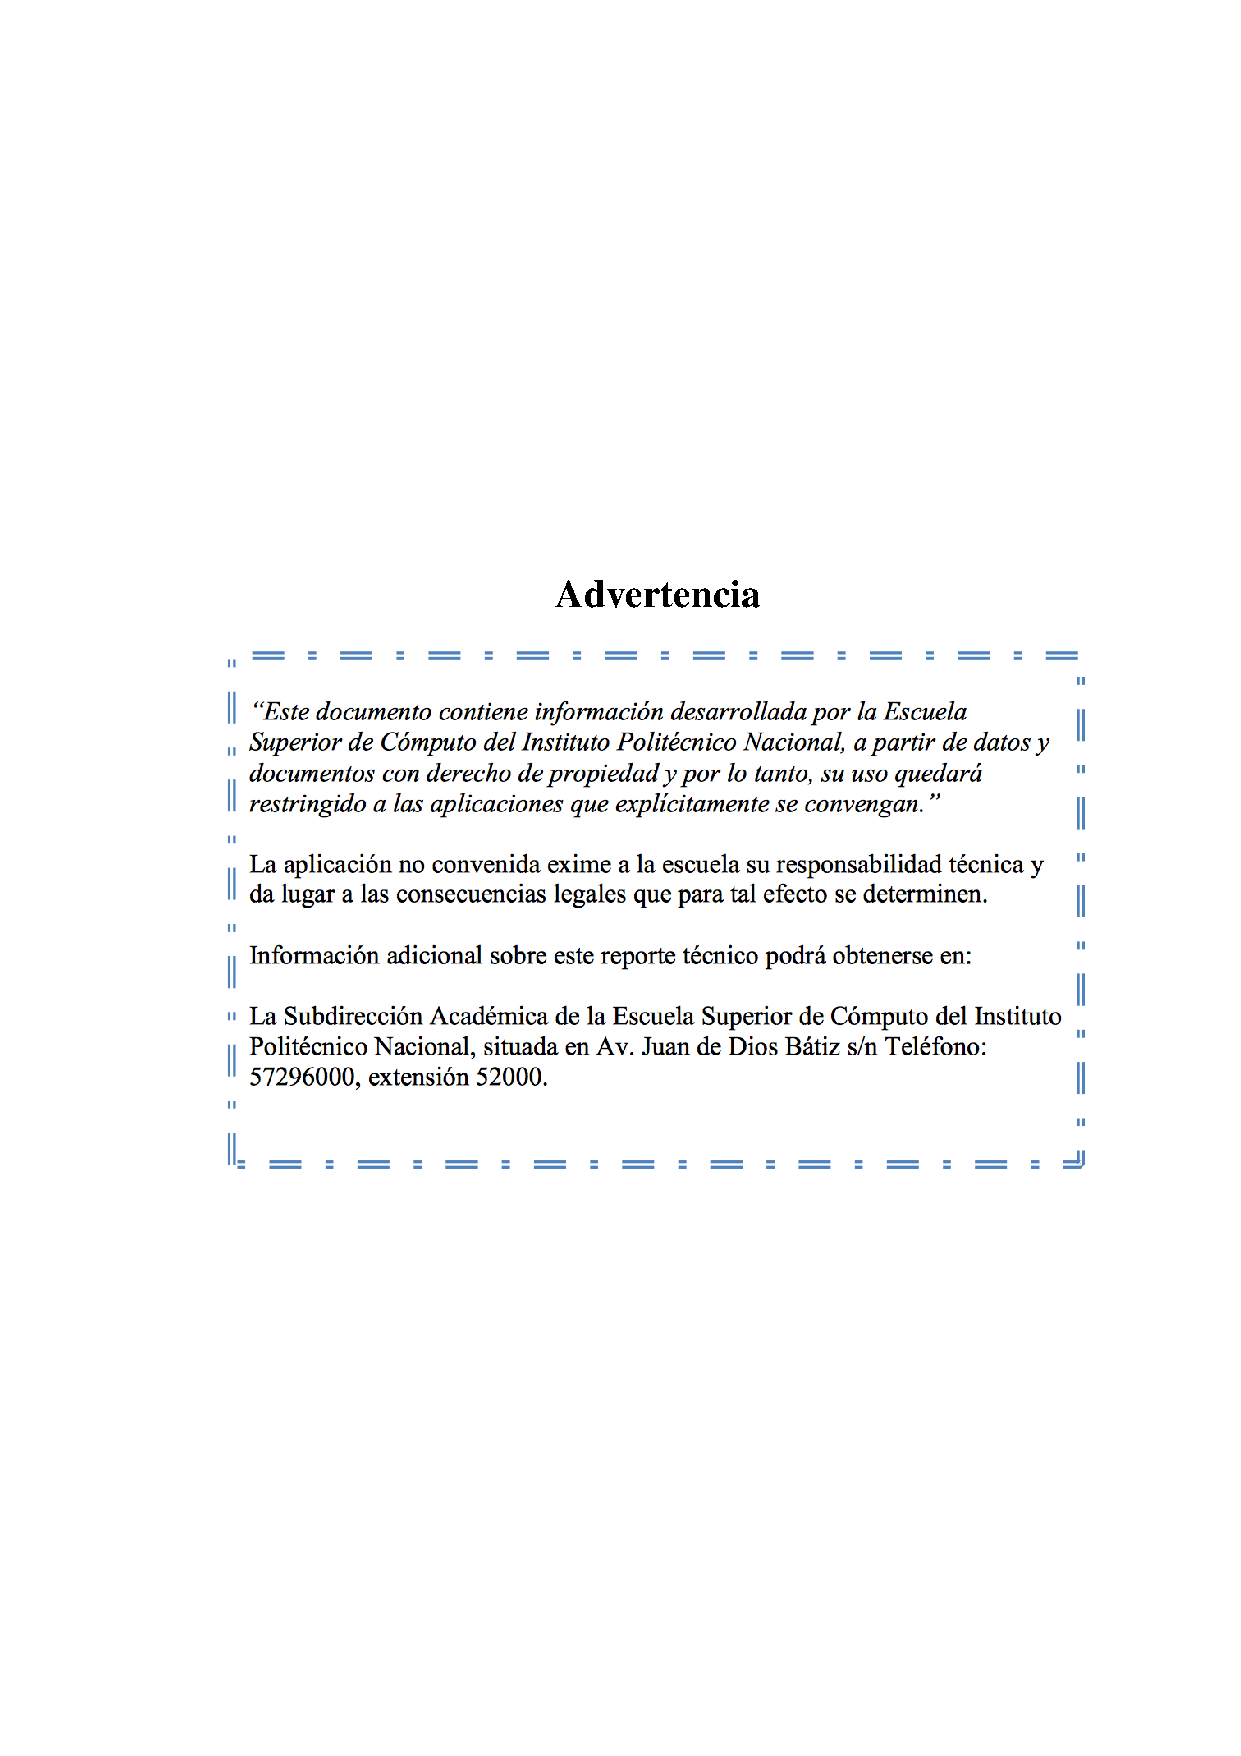
\includepdf{frontmatter/advertencia}
    \chapter{Agradecimientos}
Este proyecto no habría sido posible sin el apoyo, guía y motivación de muchas personas e instituciones a lo largo de este camino. A todas ellas, quiero expresar mi más profundo agradecimiento.

En primer lugar, mi gratitud infinita a mis directores, el \textbf{Maestro Saúl de la O Torres} y el \textbf{Doctor Gabriel Sepúlveda Cervantes}, por su invaluable guía, dedicación y apoyo constante. Su experiencia y compromiso no solo orientaron este trabajo, sino que también dejaron una huella imborrable en mi formación profesional.

Al \textbf{Instituto Politécnico Nacional}, por abrirme sus puertas y brindarme durante los últimos seis años un espacio para crecer, aprender y soñar. Gracias por proporcionarme las herramientas, conocimientos y valores necesarios para poner la técnica al servicio de la patria y contribuir a un mundo mejor.

A mi familia, que ha estado conmigo en las buenas, en las malas y en las peores, mi más sincero agradecimiento. A mi madre, \textbf{María Luisa Aguayo Torres}, mi mayor inspiración y guía. Su amor incondicional y esfuerzo incansable han sido la base de cada logro que he alcanzado. A mi padre, \textbf{Luis Carlos García Alaniz}, por su apoyo constante y por estar presente cuando más lo he necesitado. A mis hermanos, \textbf{Carlos Pavel Cuauhtémoc Tupac Amaru} y \textbf{María Sachenka América Libertad}, por ser una fuente constante de motivación, cariño y respaldo en cada etapa de este camino.

A mis compañeros del \textbf{Laboratorio de Realidad Virtual del CIDETEC}, por hacer cada tarde más amena con sus consejos, historias y camaradería. Gracias, \textbf{Gus, Ángel, Germán, Pepe, Lalo, Mike, Gabo, Steven, Wonka y Fer}, por convertir cada jornada de trabajo en una experiencia inolvidable, llena de aprendizajes y risas.

A la \textbf{Escuela Secundaria Diurna No. 4 "Moisés Sáenz"}, por abrirme sus puertas y permitirme llevar este proyecto a la práctica, facilitando un espacio para su desarrollo y pruebas.

Al \textbf{profesor Ernesto Ángel Uribe Pérez}, por su generosidad al compartir su vasto conocimiento en química, sus valiosas ideas y su apoyo constante. Su experiencia fue un aporte esencial para el éxito de este proyecto.

A la alumna \textbf{Castro Gordillo Miranda} del grupo \textbf{3° A}, por su dedicación y tiempo en la realización de las pruebas que contribuyeron significativamente al desarrollo del simulador.

Finalmente, a todos los profesores que he tenido el honor de tener a lo largo de mi formación académica. Su dedicación y pasión por la enseñanza dejaron en mí una semilla de curiosidad y amor por el conocimiento que sigue creciendo cada día.

Este logro es el resultado de un esfuerzo colectivo y una suma de voluntades.
\newpage
    \pagestyle{empty}
    \phantomsection % Crea un marcador para el enlace en el índice
\addcontentsline{toc}{chapter}{Carta De Autorización De Difusión En El Repositorio Institucional De Tesis} % Añade al índice
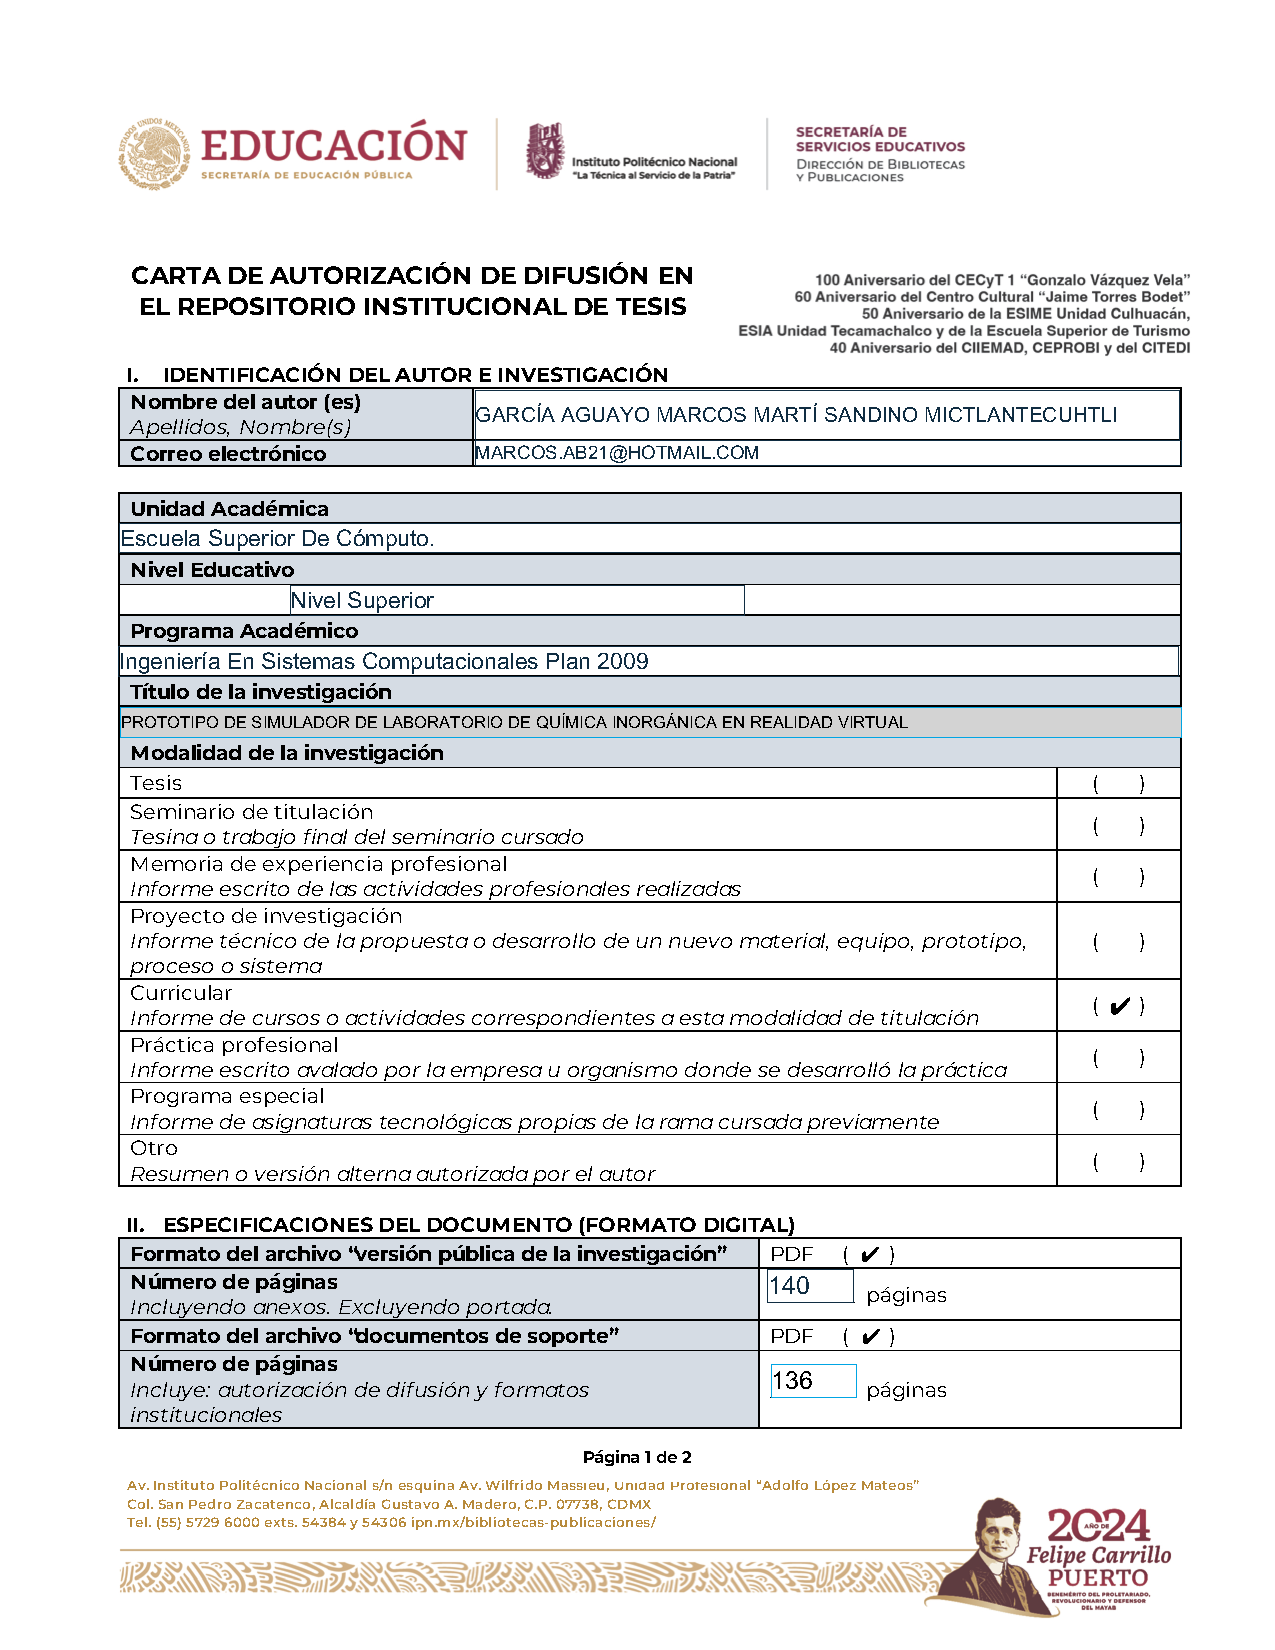
\includepdf[pages={1-2}]{frontmatter/carta}
    \pagestyle{headings}
    \tableofcontents
    \listoffigures
    \listoftables

\mainmatter
    \chapter{Introducción}\label{ch:Introducción}

\section{Antecedentes}
En las últimas décadas, el avance tecnológico ha permeado de manera significativa en diversos ámbitos de la sociedad, transformando la forma en que interactuamos con el mundo que nos rodea. Uno de los campos donde esta revolución ha sido más evidente es en el ámbito educativo, donde la integración de la tecnología se ha convertido en un tema de relevancia ineludible. Brito \cite{Brito2015} resalta que la emergencia de la cultura digital ha traído consigo profundas transformaciones en la forma en que concebimos la producción, circulación y apropiación del conocimiento, desafiando las estructuras y valores culturales previamente establecidos.

A lo largo del siglo XX, se han iniciado programas para incorporar herramientas tecnológicas en las escuelas de educación básica en México, pero su éxito tanto en términos operativos como pedagógicos ha sido limitado. Esto se atribuye, en parte, a la rigidez de las instituciones escolares, las cuales han enfrentado dificultades para replantear los modelos de socialización que tradicionalmente han prevalecido en el ámbito educativo\cite{Trejo-Quintana2020}.

La llegada de internet, las computadoras y los dispositivos digitales ha abierto un abanico de posibilidades en la educación. La revolución tecnológica de las últimas cuatro décadas ha llevado a la necesidad de integrar dispositivos de comunicación e información en los procesos educativos, considerándose incluso como la única vía para expandir el acceso al conocimiento de manera eficiente y veloz\cite{Trejo-Quintana2020}.

En este entorno, la educación STEM (Ciencia, Tecnología, Ingeniería y Matemáticas), se presenta como un pilar fundamental. Este enfoque interdisciplinario no solo se limita al ámbito académico, sino que también incorpora contextos y situaciones relevantes para la vida cotidiana de los estudiantes, así como los materiales necesarios para su comprensión y aplicación\cite{Sanchez2018}. Desde la perspectiva de Zamorano Escalona, García Cartagena y Reyes González \cite{Zamorano2018}, la educación STEM, o STEAM al incluir las Artes, busca nutrir a la industria científica y tecnológica con recursos humanos creativos. Esto se logra al aumentar el interés de los estudiantes y al desarrollar habilidades esenciales del siglo XXI, fundamentales para estimular el progreso científico-tecnológico, a través de una integración interdisciplinaria de ciencias, tecnología, matemáticas, artes e ingeniería que vincula los contenidos con las experiencias de vida de los estudiantes.

La introducción de la realidad virtual (RV) en este contexto educativo no solo representa un avance tecnológico, sino una oportunidad para superar barreras y maximizar el potencial de la enseñanza. Aunque es cierto que la accesibilidad a esta tecnología puede ser un desafío, su implementación estratégica abre un abanico de posibilidades educativas inexploradas. La RV no solo ofrece experencias inmersivas, sino que también brinda la capacidad de simular situaciones y entornos complejos. Esto la convierte en una herramienta invaluable para la capacitación, investigación y creación de soluciones innovadoras, no solo en el ámbito académico sino también en la industria y el mundo profesional \cite{Zapatero2011}.

\section{Planteamiento del Problema}
Ante la falta de interés y comprensión en la química inorgánica entre los estudiantes, se plantea el desarrollo de un prototipo de simulador de laboratorio en realidad virtual. Esta herramienta busca ofrecer una experiencia educativa más interactiva y atractiva, permitiendo a los estudiantes interactuar con elementos químicos y comprender conceptos tanto básicos como clave en un entorno virtual controlado. El objetivo es revitalizar el interés por esta materia y mejorar el aprendizaje de esta disciplina.

\section{Solución Propuesta}
Un prototipo de simulador de laboratorio de química inorgánica en realidad virtual. Los usuarios podrán realizar experimentos específicos, interactuar con los elementos y observar las reacciones en un entorno controlado.

\begin{itemize}
  \item Prototipo de Simulador en Realidad Virtual de Química Inorgánica que consta de:
    \begin{itemize}
        \item Tabla periódica interactiva.
        \item Interfaz de usuario.
        \item Algoritmos de simulación.
        \item Ejercicios de química inorgánica.
    \end{itemize}
  \item Documentación Técnica.
  \item Manual de Usuario.
  \item Pruebas y validación.
\end{itemize}

\begin{figure}[thbp]
    \centering
    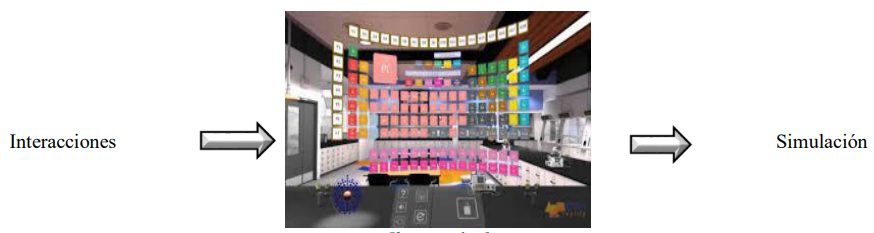
\includegraphics[width=\textwidth]{img/chapter01/Sistema.png}
    \caption{Esquema de Solución.}\label{fig:Esquema}
\end{figure}
\newpage
\section{Objetivos}

\subsection{General}
Desarrollar un prototipo de simulador en realidad virtual que permita a los usuarios interactuar con elementos químicos, combinarlos y observar sus reacciones en un entorno virtual controlado. Este simulador proporcionará una representación visual y práctica de los conceptos clave de la química inorgánica, con el propósito de complementar la comprensión teórica sin sustituir la experimentación en el laboratorio. Limitado a un contexto demostrativo, no esta diseñado para su implementación en entornos educativos formales.


\subsection{Específicos}
\begin{enumerate}[i]
  \item Modelado e integración de una tabla periódica interactiva para una selección dináminca de elementos químicos.
  \item Diseño de la Interfaz de Usuario (IU) para una interacción intuitiva con elementos químicos.
  \item Desarrollo e implementación de algoritmos de simulación para la experimentación virtual y observación de reacciones químicas interactivas.
  \item Crear ejercicios de complejidad progresiva para el aprendizaje de conceptos de química inorgánica.
  \item Pruebas y validación del simulador para una experiencia de usuario satisfactoria.
\end{enumerate}

\section{Justificación}
En el ámbito educativo, se identifica la necesidad apremiante de enriquecer la enseñanza de las ciencias, específicamente la química, entre los jóvenes. A pesar de la disponibilidad de múltiples fuentes de información y recursos audiovisuales para complementar el aprendizaje, persiste la preocupación por la falta de interés de un considerable número de jóvenes en las ciencias. Esta apatía hacia la disciplina puede estar obstaculizando la comprensión profunda y el entusiasmo por aprender sobre la química inorgánica.

En respuesta a este desafío, el proyecto propone una solución innovadora. Mediante una experiencia educativa e interactiva en realidad virtual, se busca abordar la falta de interés al ofrecer una perspectiva diferente y cautivadora de la disiplina. Al proporcionar a los jóvenes una herramienta que les permita interactuar con elementos químicos, combinarlos y observar sus reacciones en un entorno virtual controlado, se fomenta una comprensión más práctica y atractiva de los conceptos.

Esta iniciativa no solo complementa el aprendizaje teórico, sino que también busca revitalizar la motivación intrínseca de los estudiantes hacia las ciencias, en particular la química. Al hacerlo, se aspira a cultivar un ambiente de aprendizaje más estimulante y participativo, que inspire a los estudiantes a explorar y comprender de manera más profunda los principios fundamentales de la química inorgánica.

\newpage
\section{Estado del arte}

\subsection{VRLab Academy}
VRLab Academy se destaca como una empresa líder en innovación tecnológica educativa, especializada en el desarrollo de contenido de experimentos de realidad virtual con propósitos científicos y educativos. Su compromiso se centra en proporcionar a los estudiantes una experiencia de laboratorio virtual auténtica que les permita llevar a cabo experimentos y mejorar sus habilidades en un entorno interactivo, seguro y educativo.

\begin{figure}[thbp]
    \centering
    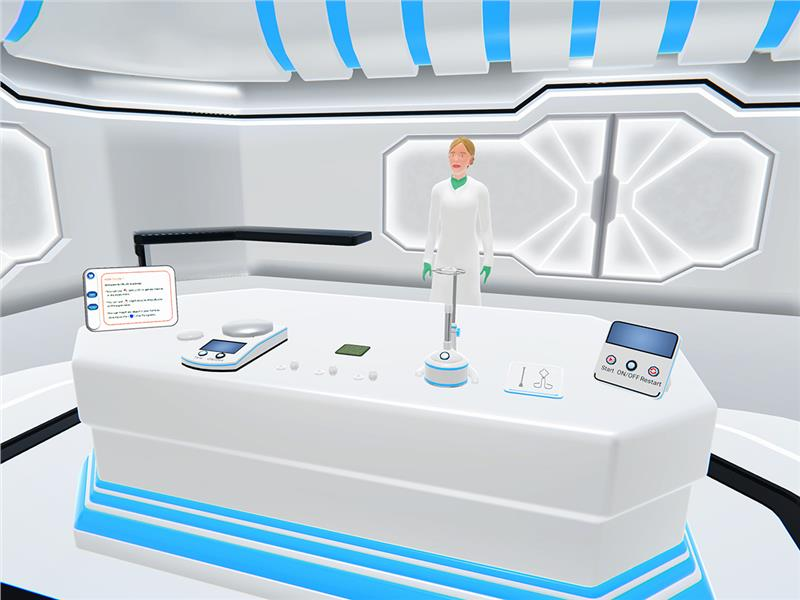
\includegraphics[width=0.8\textwidth, height=8cm]{img/chapter01/Chemistry_Lab_-_VRLab_Academy.jpg}
    \caption{Simulador VRLab Academy.}\label{fig:Esquema}
\end{figure}

El enfoque de VRLab Academy se basa en la utilización de datos en tiempo real, fórmulas científicas verídicas y resultados reales. Los estudiantes tienen la capacidad de guardar y compartir los datos obtenidos durante sus experimentos.

La plataforma de VRLab Academy ofrece dos versiones de sus experimentos: VR y PC. La versión de realidad virtual requiere un dispositivo de realidad virtual como Oculus o HTC, mientras que la versión para PC solo necesita una computadora o portátil con conexión a Internet. Esta variedad de opciones permite adaptarse a las diferentes necesidades y recursos disponibles para los estudiantes.

\newpage
\subsection{Garg Lab VR Chem}

Grag Lab VR Chem es una iniciativa desarrollada por el equipo de químicos orgánicos de la Universidad de California, Los Ángeles (UCLA). Esta plataforma de realidad virtual ha sido creada con el propósito de mejorar el aprendizaje de la química orgánica, ofreciendo a los estudiantes la posibilidad de interactuar con modelos moleculares en un entorno tridimensional.

La aplicación guía a los estudiantes a través de un entorno virtual donde pueden interactuar con modelos moleculares en 3D. Cada molécula viene acompañada de información relevante sobre su función y su presencia en la vida cotidiana, proporcionando contexto adicional para el aprendizaje.

\begin{figure}[thbp]
    \centering
    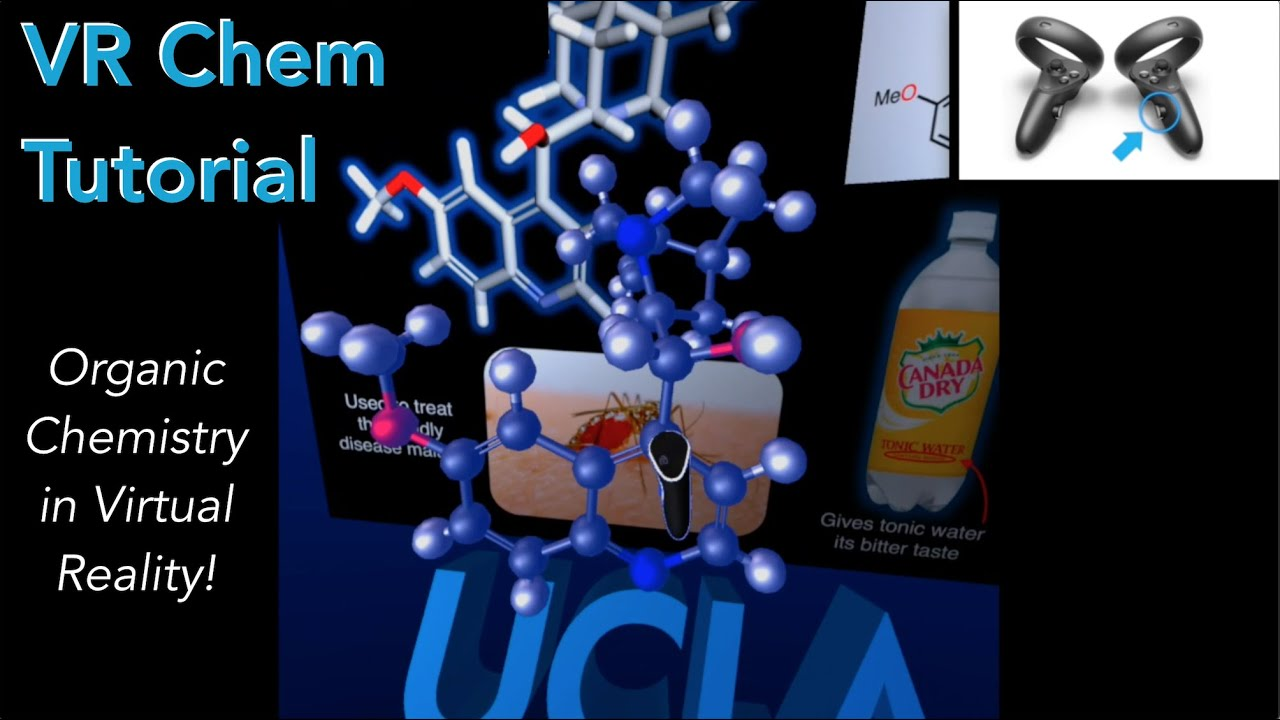
\includegraphics[width=0.8\textwidth, height=8cm]{img/chapter01/Garg_Lab_VR_Chem.jpg}
    \caption{Aplicación VR Chem.}\label{fig:Esquema}
\end{figure}

VR Chem ofrece una ventaja significativa en la comprensión de las estructuras moleculares en 3D, ya que permite a los estudiantes modelar moléculas complejas de una manera interactiva. La aplicación es compatible con una variedad de dispositivos de realidad virtual, incluyendo HTC VIVE, Windows Mixed Reality, Oculus Rift, Oculus Quest, PlayStation VR y Valve Index.

\newpage
\subsection{PraxiLabs}

PraxiLabs es una plataforma educativa que ofrece laboratorios virtuales interactivos en diversas disciplinas científicas, incluyendo química. Esta innovadora plataforma permite a los estudiantes llevar a cabo experimentos virtuales de laboratorio sin la necesidad de contar con equipo físico. De esta manera, PraxiLabs ofrece una experiencia práctica segura y accesible desde cualquier lugar con conexión a Internet.

Se trata de un laboratorio virtual en 3D que ofrece simulaciones de física, química y biología, diseñado para facilitar el proceso de enseñanza de la ciencia tanto para educadores como para estudiantes.

PraxiLabs funciona en computadoras de escritorio y portátiles.

\begin{figure}[thbp]
    \centering
    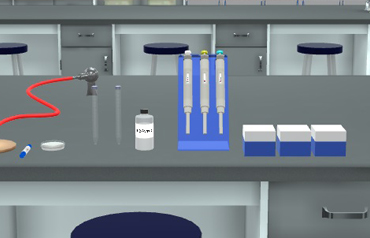
\includegraphics[width=0.8\textwidth, height=8cm]{img/chapter01/Praxi Labs.jpg}
    \caption{Praxi Labs - Laboratorio de Química Inorgánica.}\label{fig:Esquema}
\end{figure}

Se requiere una conexión a Internet confiable para cargar los experimentos. La velocidad de la conexión determina la rapidez de carga. Una vez que el experimento está cargado, no es necesario seguir conectado a Internet, a menos que se utilicen archivos multimedia proporcionados.

\newpage
\subsection{Laboratorio Virtual de Experimentación Química UPM}

El Laboratorio Virtual de Experimentación Química de la UPM es una herramienta educativa que simula un laboratorio real para realizar prácticas de análisis de elementos tóxicos en muestras de suelo. Esta alternativa virtual ofrece mayor seguridad y eficiencia que las prácticas presenciales, ya que reduce riesgos y tiempos de experimentación.

Los estudiantes participan en dos etapas de práctica. En la primera, acceden a material audiovisual y al quimitrivial-UPM desde mesas con ordenadores, además de utilizar un laboratorio equipado con instrumentos básicos de química. Una vez completada esta fase, acceden a los módulos de preparación e instrumentación, donde realizan un procedimiento real para determinar elementos tóxicos en muestras de suelo contaminado. Esto incluye la mineralización de la muestra en un horno de microondas y el análisis por ICP-AES.

\begin{figure}[thbp]
    \centering
    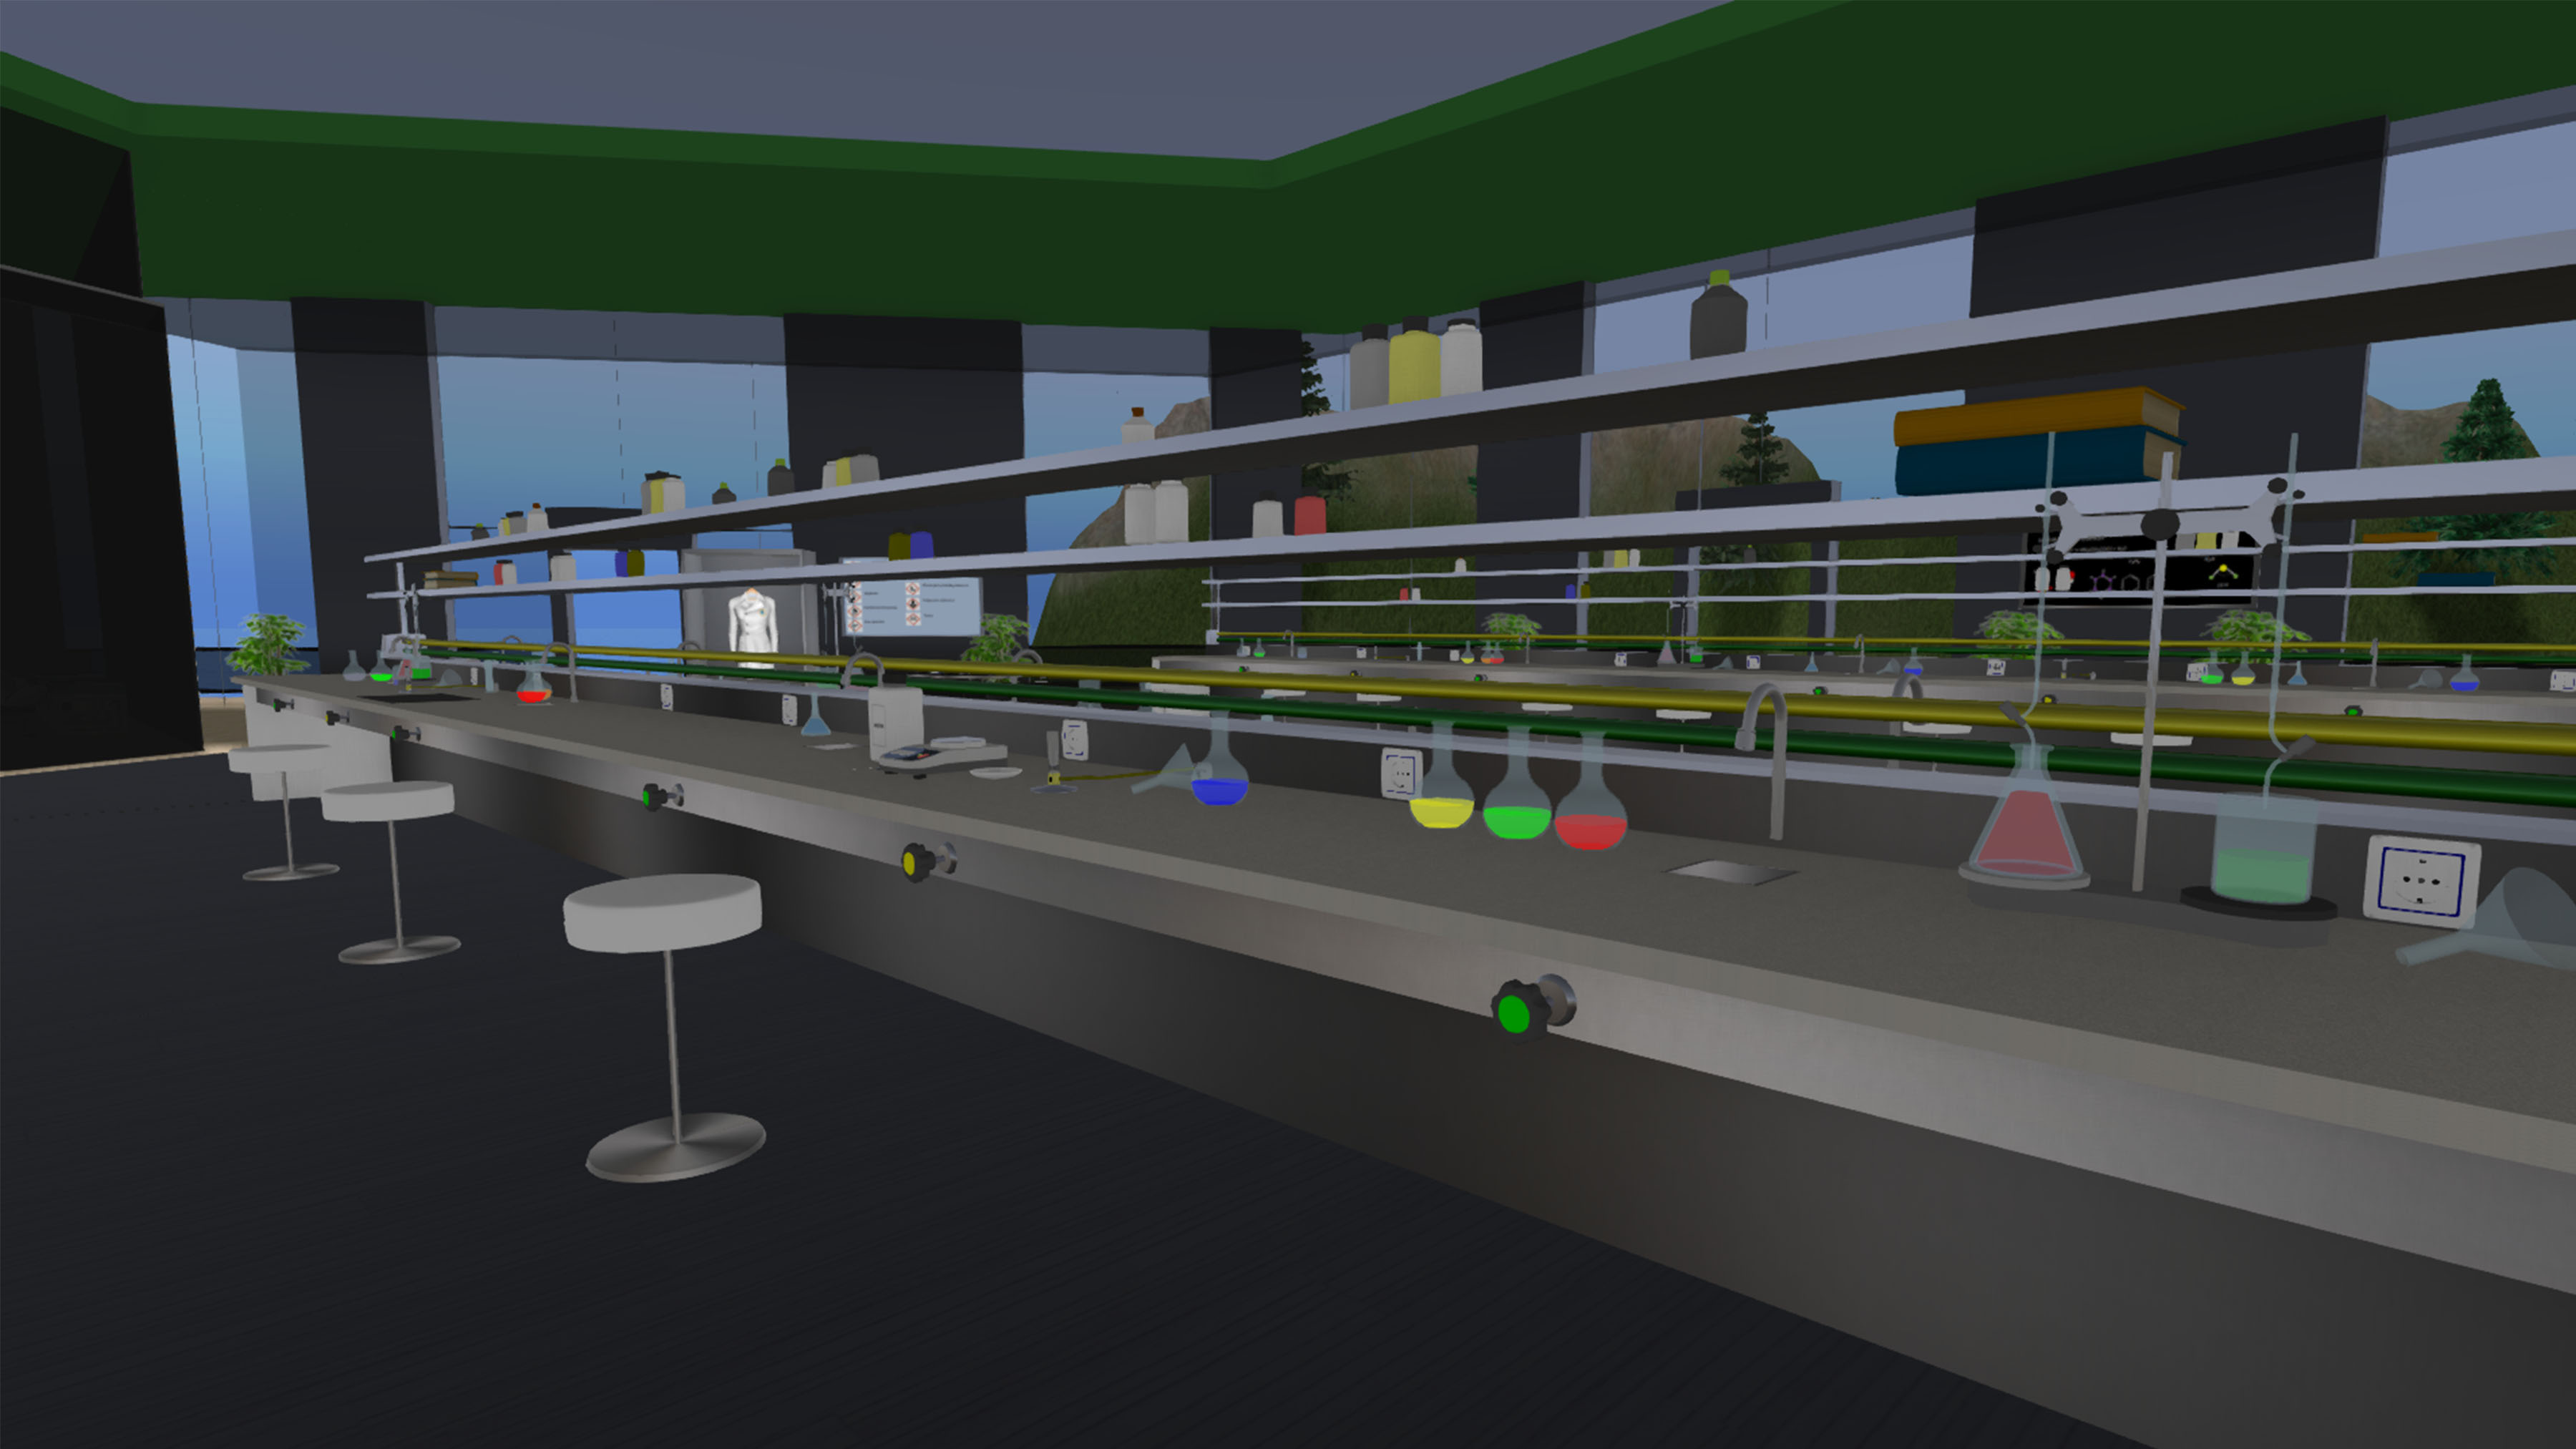
\includegraphics[width=0.8\textwidth, height=8cm]{img/chapter01/UPM.jpg}
    \caption{Experimentación Química UPM.}\label{fig:Esquema}
\end{figure}

Los estudiantes ingresan al laboratorio virtual desde sus ordenadores utilizando sus cuentas institucionales UPM con el Sistema de Inicio de Sesión Único (SSO). La plataforma, construida en Unity 3D y exportada en WebGL, es accesible a través de la mayoría de los navegadores comerciales, sin descargas adicionales. Todo el contenido necesario se descarga automáticamente al conectarse, con una barra de carga indicando el progreso.

\newpage
\subsection{EVA Tech}

Evatech es una plataforma de realidad virtual diseñada para abordar problemas mediante conocimientos científicos. Con un enfoque multidisciplinario, fusiona tecnología, creatividad, pensamiento crítico y habilidades de comunicación.

Esta innovadora herramienta promueve el desarrollo de competencias STEM a través de sesiones de trabajo en equipo en realidad virtual. Dirigida a estudiantes de secundaria y preparatoria, las sesiones interactivas de Evatech refuerzan conceptos científicos y fomentan el aprendizaje práctico y colaborativo.

\begin{figure}[thbp]
    \centering
    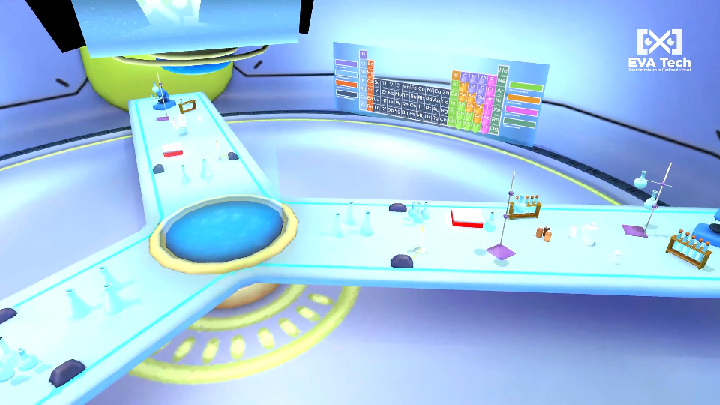
\includegraphics[width=0.8\textwidth, height=8cm]{img/chapter01/Eva_Tech.png}
    \caption{Módulo Química.}\label{fig:Esquema}
\end{figure}

Al utilizar la realidad virtual, Evatech ofrece una experiencia educativa emocionante y efectiva, estimulando nuevas conexiones neuronales al conectar el cuerpo con el razonamiento. Su enfoque en el desarrollo de habilidades motrices y el uso de tecnologías del futuro garantiza un aprendizaje innovador y comprometido con el progreso educativo.

\newpage
\subsection{HoloLab Champions}

HoloLAB Champions es un programa de juegos de realidad virtual que transporta a los jugadores a un laboratorio virtual, donde aprenden habilidades prácticas reales para realizar experimentos. Los jugadores compiten en minilabs organizados por Earl, el presentador holográfico con un sentido del humor ingenioso. Diseñado para estudiantes de 14 a 18 años, este juego de un solo jugador puede ser utilizado en entornos grupales en el aula, donde un estudiante juega mientras otros observan, brindan asistencia y toman notas, con la guía del maestro.

El juego consta de dos episodios de 30 a 40 minutos cada uno, diseñados para enseñar habilidades básicas de laboratorio, procedimientos y protocolos. El primer episodio, Chemiluminescence, enseña a los estudiantes a mezclar ingredientes líquidos y sólidos para crear una solución química brillante. El segundo episodio, Identify Unknowns, desafía a los jugadores a identificar correctamente diversas sustancias con información de referencia limitada.

\begin{figure}[thbp]
    \centering
    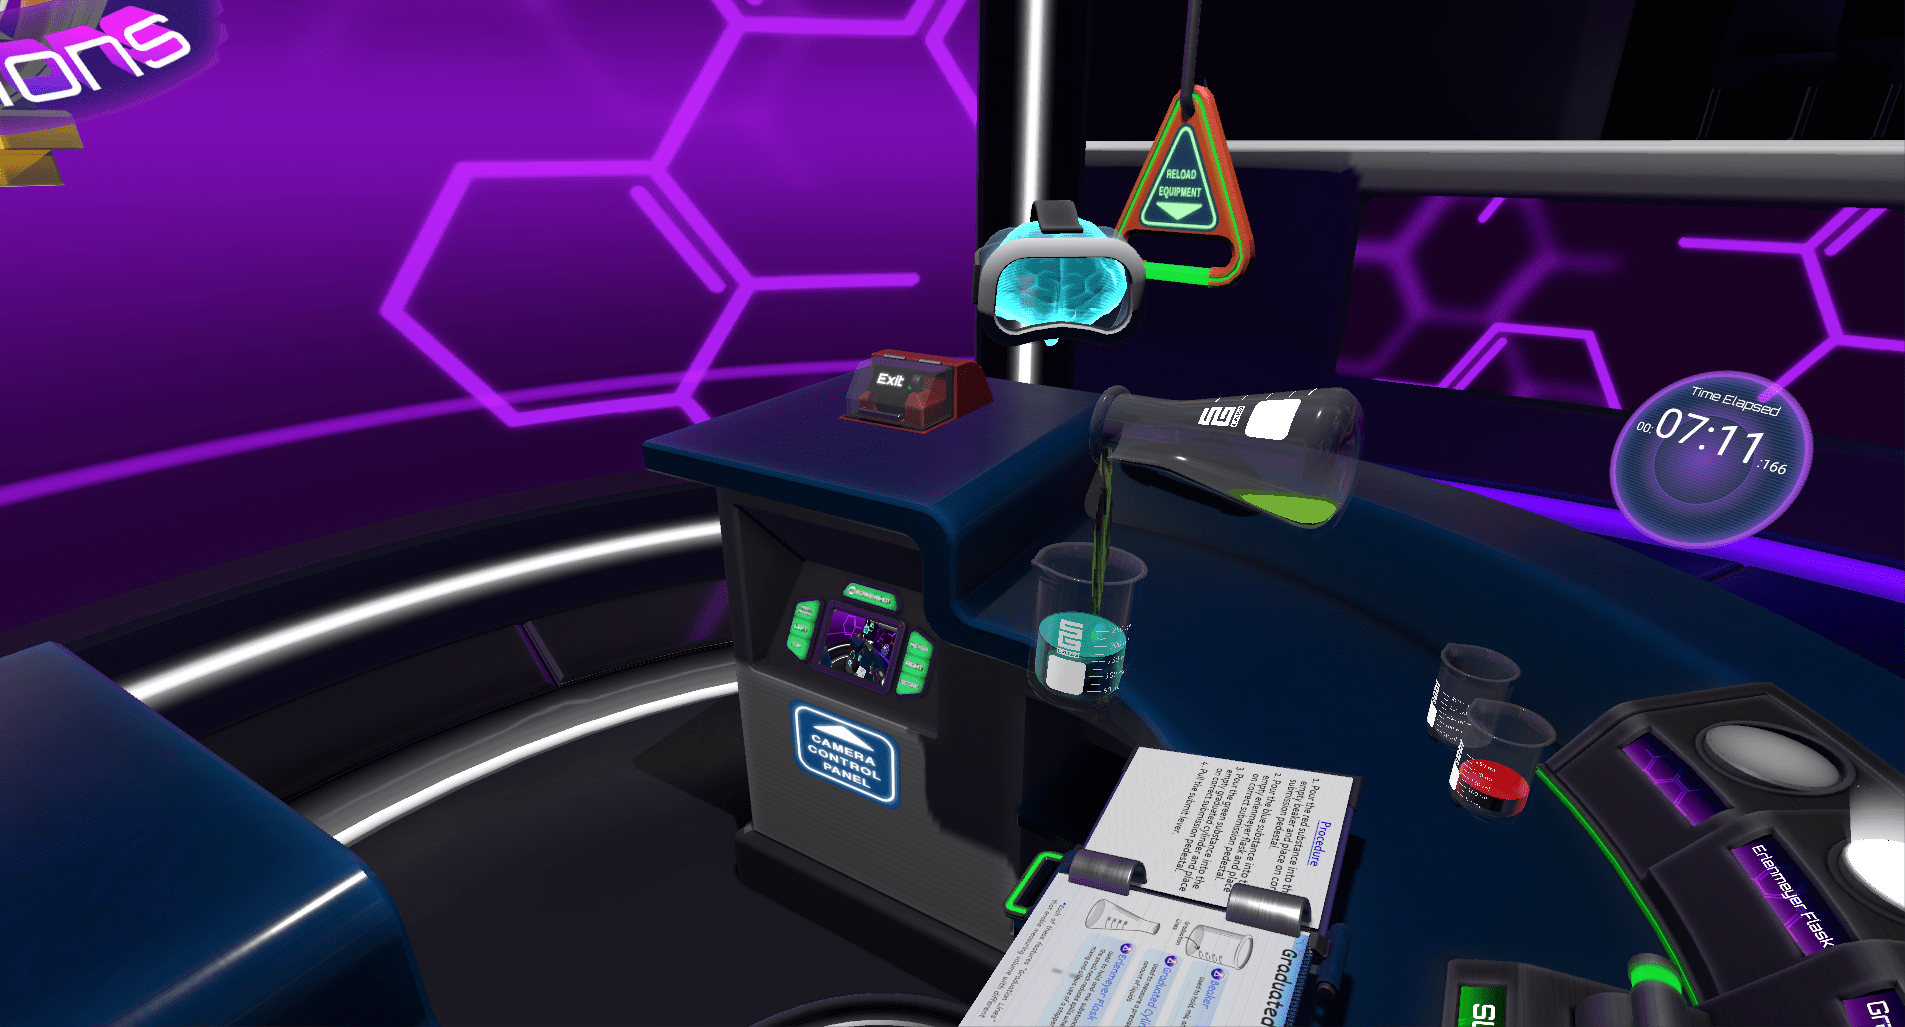
\includegraphics[width=0.8\textwidth, height=8cm]{img/chapter01/hololab-champions_pouring-min.png}
    \caption{HoloLab Champions - Chemiluminescence.}\label{fig:Esquema}
\end{figure}

Financiado parcialmente por una subvención SBIR del Instituto de Ciencias de la Educación del Departamento de Educación de los Estados Unidos, HoloLAB Champions fue desarrollado en asociación con estudiantes, educadores y la RAND Corporation, siguiendo un proceso iterativo para garantizar su efectividad y utilidad educativa.

\newpage
\subsection{Tabla Comparativa}

\begin{table}[H]
  \centering
  \begin{tabular}{|>{\centering\arraybackslash}m{.2\textwidth}|>{\centering\arraybackslash}m{.1\textwidth}|>{\centering\arraybackslash}m{.1\textwidth}|>{\centering\arraybackslash}m{.15\textwidth}|>{\centering\arraybackslash}m{.15\textwidth}|>{\centering\arraybackslash}m{.15\textwidth}|}
    \hline
    \rowcolor{blue_escom}
    Simulador &  Realidad Virtual (VR) &  Hand Tracking &  Etapas Integradas & Idioma & Público Objetivo
 \\
    
    \hline
    \cellcolor{column_color}VRLab Academy & ✓ & ✗ & Visualización, Experimentación & Varios & Estudiantes de Preparatoria y Universidad \\
    
    \hline
    \cellcolor{column_color}Garg Lab VR Chem & ✓ & ✗ & Visualización & Inglés & Estudiantes de pregrado\\
    
    \hline
    \cellcolor{column_color}PraxiLabs & ✗ & ✗ & Experimentación & Inglés y Árabe & Estudiantes de ciencias\\
    
    \hline
    \cellcolor{column_color}Laboratorio Virtual de Experimentación Química UPM & ✗ & ✗ & Balanceo de ecuaciones, Experimentación & Español & Estudiantes universitarios\\
    
    \hline
   \cellcolor{column_color} EVA Tech & ✓ & ✗ & Visualización & Español & Estudiantes de Nivel Básico\\
   
    \hline
    \cellcolor{column_color}HoloLab Champions & ✓ & ✗ & Experimentación & Inglés & Adolescentes y Adultos\\
    
    \hline
    \cellcolor{column_color}TT-2024-B059 & ✓ & ✓ & Visualización, Balanceo de ecuaciones, Creación de compuestos, Experimentación & Español & Adolescentes\\
    \hline
  \end{tabular}
  \caption{Comparativa de simuladores de laboratorios virtuales}
  \label{tab:comparativa}
\end{table}

    \chapter{Marco Teórico}\label{ch:Marco_Teórico}

\section{Química}
La química es la ciencia que estudia la materia, su composición, estructura, propiedades y las transformaciones que experimenta. En el contexto de este proyecto, nos centraremos en los aspectos de la química inorgánica relevantes para los experimentos que se simularán en el entorno virtual. 

\subsection{Química Inorgánica}

Constituye una de las ramas principales de la química, enfocada en el estudio de los elementos y compuestos que no contienen carbono, excluyendo así los compuestos orgánicos. Su ámbito de estudio abarca desde la comprensión de las propiedades básicas de los elementos individuales hasta la síntesis y caracterización de compuestos inorgánicos complejos.

\subsection{Reacciones Químicas}
Las reacciones químicas representan procesos en los cuales sustancias reactantes se transforman en otras sustancias, denominadas productos. Estas transformaciones se expresan mediante ecuaciones químicas, donde las fórmulas de los reactivos se encuentran en el primer miembro y las de los productos en el segundo. Los coeficientes en estas ecuaciones indican las proporciones molares de las sustancias participantes \cite{alfa_nauta}.

\begin{itemize}
    \item \textit{\textbf{Reacciones de Oxidación-Reducción (Redox): }}
    Una reacción de oxidación-reducción (redox) es un tipo de reacción química que implica la transferencia de electrones entre dos especies. La especie que pierde electrones se oxida, mientras que la especie que gana electrones se reduce. Estas reacciones son fundamentales en muchos procesos químicos y biológicos, y su comprensión es crucial para el estudio de la química. 

    En una reacción redox, el número de electrones perdidos por la especie que se oxida debe ser igual al número de electrones ganados por la especie que se reduce. Esto se debe a la ley de conservación de la masa, que establece que la materia no se crea ni se destruye en una reacción química, solo se transforma. 
    
    Para identificar una reacción redox, se pueden utilizar los números de oxidación, que indican el estado de oxidación de un átomo en un compuesto. El número de oxidación de un átomo puede ser positivo, negativo o cero, y representa la carga hipotética que tendría el átomo si todos sus enlaces fueran iónicos. 
    \item \textit{\textbf{Reacciones de Combustión: }}
    Las reacciones de combustión son un tipo particular de reacción redox en las que una sustancia combustible reacciona con un oxidante (generalmente oxígeno) para producir óxido del combustible y liberar energía en forma de luz y calor. 
    
    \textit{\textbf{Energía de activación y punto de ignición }}\\
    Para que una reacción de combustión se inicie, se requiere un aporte inicial de energía, llamada energía de activación. Esta energía puede provenir de una llama, chispa o fuente de calor. Una vez iniciada la reacción, la energía liberada en forma de calor es suficiente para mantener la combustión hasta que se agote el combustible. 
    El punto de ignición es la temperatura mínima a la que una sustancia combustible debe ser calentada para iniciar la combustión en presencia de oxígeno. Cada combustible tiene un punto de ignición específico.  
    \begin{itemize}
        \item \textit{\textbf{Reacciones exotérmicas:}} Liberan energía al entorno en forma de calor.
        \item \textit{\textbf{Reacciones endotérmicas:}} Absorben energía del entorno.
    \end{itemize}
    \item \textit{\textbf{Reacciones de Síntesis: }}
    Una reacción de síntesis es aquella en la que dos o más sustancias (reactivos) se combinan para formar un único producto. En general, estas reacciones siguen el patrón: A + B → AB
\end{itemize}

\subsection{Estequiometría}
La estequiometría es una herramienta esencial en química que permite analizar las relaciones cuantitativas entre reactivos y productos en una reacción química. Se basa en el concepto de mol, que es la unidad fundamental de cantidad de sustancia en el Sistema Internacional de Unidades (SI). Un mol de cualquier sustancia contiene el mismo número de entidades elementales (átomos, moléculas, iones, etc.), conocido como número de Avogadro ($6.022 * 10^{23}$)\cite{Estequiometria}. 
    
La estequiometría se utiliza para: 
    
\textbf{Balancear ecuaciones químicas:} Ajustar los coeficientes de una ecuación química para que el número de átomos de cada elemento sea el mismo en ambos lados de la ecuación, cumpliendo así con la ley de conservación de la masa. 
    
\textbf{Calcular relaciones molares:} Determinar la cantidad de moles de una sustancia que reaccionan con una cantidad dada de otra sustancia, o la cantidad de moles de producto que se forman a partir de una cantidad dada de reactivo. 
    
\textbf{Calcular relaciones de masa:} Convertir entre masa y moles de una sustancia utilizando la masa molar, que es la masa de un mol de esa sustancia. 
    
\textbf{Calcular el rendimiento de una reacción:} Determinar la cantidad de producto que se obtiene en una reacción química en comparación con la cantidad teórica que se debería obtener según la estequiometría. 
    
La estequiometría es una herramienta fundamental en el laboratorio, ya que permite a los químicos diseñar experimentos, predecir los resultados y analizar los datos obtenidos. 

\subsection{Cinética Química}
La cinética química es el estudio de la velocidad de las reacciones químicas y los factores que la afectan. La velocidad de una reacción se define como el cambio en la concentración de un reactivo o producto por unidad de tiempo\cite{Cinetica_Quimica_Basica}. 

Los factores que afectan la velocidad de una reacción química incluyen: 

\begin{itemize}
    \item \textbf{Concentración de los reactivos:} En general, la velocidad de una reacción aumenta a medida que aumenta la concentración de los reactivos. Esto se debe a que una mayor concentración de reactivos significa que hay más moléculas disponibles para colisionar y reaccionar. 

    \item \textbf{Temperatura:} La velocidad de una reacción generalmente aumenta a medida que aumenta la temperatura. Esto se debe a que las moléculas se mueven más rápido a temperaturas más altas, lo que aumenta la frecuencia y la energía de las colisiones. 

    \item \textbf{Catalizadores:} Un catalizador es una sustancia que aumenta la velocidad de una reacción química sin consumirse en ella. Los catalizadores funcionan al proporcionar un camino de reacción alternativo con una menor energía de activación. 
\end{itemize}

\subsection{Ley de Rapidez}
La ley de rapidez, también conocida como ecuación de velocidad, describe la relación matemática entre la velocidad de una reacción química y la concentración de los reactivos. Esta ley se expresa de la siguiente manera: 

Velocidad de reacción = $k[A]^m[B]^n...$ 
 

Donde: 

k: Es la constante de velocidad de la reacción, que depende de la temperatura y la naturaleza de los reactivos. 

[A], [B], ...: Son las concentraciones molares de los reactivos A, B, etc. 

m, n, ...: Son los órdenes de reacción respecto a cada reactivo, que indican cómo la concentración de cada reactivo afecta la velocidad de la reacción. Estos órdenes de reacción se determinan experimentalmente. 

La ley de rapidez es una herramienta fundamental en la cinética química, ya que permite predecir cómo cambiará la velocidad de una reacción al variar las concentraciones de los reactivos.

\subsection{Leyes ponderales}
También conocidas como leyes de las combinaciones químicas, son principios fundamentales que describen las relaciones cuantitativas entre los reactantes y productos en las reacciones químicas. Estas leyes fueron establecidas por John Dalton a principios del siglo XIX y sentaron las bases para la estequiometría, la rama de la química que se ocupa de las relaciones cuantitativas en las reacciones químicas\cite{Fernando2021}.
\newpage
\textbf{\textit{Ley de la Conservación de la Masa}}\\
En toda reacción química ordinaria, la masa total de los reactantes es igual a la masa total de los productos. Esto significa que la materia no se crea ni se destruye durante la reacción, solo se transforma de una forma a otra.
\\\\
\textbf{\textit{Ley de las Proporciones Definidas}}\\
Los elementos químicos se combinan para formar compuestos en proporciones fijas y definidas. Esto significa que la composición de un compuesto puro siempre es la misma, independientemente de cómo se haya obtenido.
\\\\
\textbf{\textit{Ley de las Proporciones Múltiples}}\\
Cuando dos elementos forman más de un compuesto, las masas de uno de ellos que se combinan con una masa fija del otro elemento guardan una relación sencilla de números enteros.

\section{Simulador}
Los simuladores son herramientas fundamentales en campos diversos, donde ofrecen una recreación detallada y precisa de sistemas complejos. Al recrear sensaciones físicas y comportamientos específicos, los simuladores permiten a los usuarios experimentar situaciones de manera segura y controlada. Desde entrenamientos de pilotos hasta pruebas de diseño de productos, la simulación proporciona un entorno virtual que facilita la comprensión del comportamiento de sistemas complejos y la evaluación de estrategias de operación. Además, los simuladores son una parte crucial de la innovación y el desarrollo, al permitir experimentar con diferentes escenarios sin arriesgar recursos o vidas humanas.

\subsection{Elementos de una simulación \cite{Simulación}}
\begin{enumerate} [I. ]
    \item Definición del Sistema: 
    Antes de adentrarnos en la simulación del sistema, es crucial realizar un análisis preliminar exhaustivo. Este análisis nos permite entender la interacción del sistema con otros, identificar restricciones, determinar las variables involucradas y sus relaciones, así como establecer las medidas de efectividad y los resultados esperados.
    \item Formulación del Modelo: 
    Una vez clarificados los objetivos del estudio, pasamos a la etapa de construcción del modelo. Aquí, se definen meticulosamente todas las variables que conforman el sistema, sus interrelaciones y se elaboran diagramas de flujo que retraten de manera integral el modelo en cuestión. Este proceso es fundamental para garantizar resultados precisos y útiles.
    \item Colección de Datos: 
    La disponibilidad y accesibilidad de ciertos datos, así como la complejidad para obtener otros, pueden incidir en la formulación y desarrollo del modelo. Por ello, es crucial definir con precisión los datos necesarios para lograr los resultados deseados. Habitualmente, esta información se obtiene de registros contables, órdenes de trabajo, órdenes de compra, opiniones de expertos y, en última instancia, a través de experimentación si es imprescindible. Es fundamental esta etapa para asegurar la solidez y fiabilidad del modelo.
    \item Implementación del Modelo en la Computadora:
    Una vez que el modelo está definido, el siguiente paso implica la elección entre el desarrollo en un lenguaje de programación específico o la utilización de un paquete de software adecuado para su procesamiento en la computadora, con el fin de obtener los resultados deseados.
    \item Validación: 
    Durante esta etapa, se pueden identificar posibles deficiencias tanto en la formulación del modelo como en los datos utilizados para alimentarlo. Las formas más comunes de validar un modelo son las siguientes:
    \begin{itemize}
        \item Evaluación por expertos de los resultados de la simulación.
        \item Comparación de la precisión en la predicción de datos históricos.
        \item Evaluación de la precisión en la predicción de eventos futuros.
        \item Comprobación de la falla del modelo de simulación al utilizar datos que causen fallas en el sistema real.
        \item Aceptación y confianza en el modelo por parte de las personas que utilizarán los resultados generados por el experimento de simulación.
    \end{itemize}
    \item Experimentación: 
    Una vez validado el modelo, se procede a la experimentación. Esta fase implica la generación de los datos necesarios y la realización de análisis de sensibilidad de los indicadores pertinentes. 
    \item Interpretación: 
    Una vez completada la experimentación y obtenidos los resultados de la simulación, se procede a su interpretación. En esta fase, se analizan detalladamente los datos generados y se extraen conclusiones relevantes. Basándose en esta interpretación, se toma una decisión informada.
    \item Documentación: 
    Para maximizar el uso del modelo de simulación, se requieren dos tipos de documentación: técnica y manual de usuario. La documentación técnica detalla el funcionamiento interno del modelo, mientras que el manual de usuario proporciona instrucciones prácticas para su uso efectivo. Juntos, estos documentos garantizan que el modelo sea accesible y útil para todos los usuarios, facilitando su aplicación en diversas situaciones.
\end{enumerate}
\subsection{Beneficios}
\begin{itemize}
    \item Mayor seguridad: 
    Permiten a los usuarios practicar en entornos seguros, evitando riesgos y daños.
    \item Menor costo: 
    Su desarrollo y uso puede ser más económico que realizar experimentos en el mundo real. 
    \item Mayor control: Permiten controlar las condiciones de la simulación, lo que facilita la investigación y el análisis.
    \item Mayor accesibilidad: Pueden ser utilizados por personas que no podrían acceder a experiencias en el mundo real.
\end{itemize}
\subsection{Limitaciones}
\begin{itemize}
    \item Complejidad: 
    La creación de simuladores realistas y precisos puede ser un proceso complejo y costoso.
    \item Fidelidad: 
    Siempre tendrán un cierto grado de abstracción, lo que puede limitar su precisión.
    \item Sesgos: 
    Pueden reflejar los sesgos de sus creadores, lo que puede llevar a resultados inexactos o discriminatorios. 
\end{itemize}

\section{Realidad Virtual (RV)}
La Realidad Virtual (RV) es una tecnología que crea entornos digitales simulados e interactivos, diseñados para ser experimentados e interactuados como si fueran reales. Estos entornos se generan mediante computadoras y se presentan a los usuarios a través de dispositivos como cascos de visualización (HMD) y auriculares, sumergiéndolos en mundos virtuales tridimensionales donde pueden manipular objetos virtuales utilizando controladores de movimiento u otros dispositivos de entrada\cite{VR-Book}.
\subsection{Componentes de un Sistema de RV}
Un sistema de RV típico se compone de varios elementos clave que trabajan en conjunto para crear la ilusión de realidad:
\begin{itemize}
    \item \textit{\textbf{Dispositivos de visualización:}} Cascos de realidad virtual (HMD) que presentan imágenes estereoscópicas, engañando al cerebro para que perciba profundidad y distancia, creando la sensación de estar dentro del entorno virtual.
    \item \textit{\textbf{Dispositivos de audio:}} Auriculares o altavoces espaciales que brindan sonido envolvente, mejorando la inmersión al simular la ubicación y dirección de los sonidos en el entorno virtual.
    \item \textit{\textbf{Dispositivos de seguimiento:}} Sensores que rastrean los movimientos del usuario, como la posición de la cabeza y las manos, y los traducen en acciones dentro del entorno virtual, permitiendo una interacción natural y fluida.
    \item \textit{\textbf{Software y contenido:}} El software genera el entorno virtual, incluyendo modelos 3D, texturas, iluminación e interacciones. El contenido puede ser diverso, desde simulaciones científicas y educativas hasta juegos y experiencias artísticas.
\end{itemize}

\subsection{Inmersión e Interacción}
La inmersión es un componente fundamental de la RV y se refiere al grado en que un sistema de RV proyecta estímulos a los sentidos del usuario de manera extensa, envolvente, vívida e interactiva. La inmersión tiene como objetivo crear una sensación de presencia, donde los usuarios sientan que están realmente presentes en el entorno virtual.

La interacción en la RV es la comunicación entre el usuario y la aplicación de RV, mediada por dispositivos de entrada y salida. La fidelidad de interacción se refiere a la correspondencia entre las acciones físicas en el mundo virtual y las acciones físicas equivalentes en el mundo real. Existen interacciones realistas (alta fidelidad), no realistas (baja fidelidad) y mágicas (nivel medio de fidelidad).
\subsection{Aplicaciones de la RV en la Educación}
En el campo de la educación, la RV ofrece un enorme potencial para mejorar el aprendizaje al permitir a los estudiantes experimentar conceptos abstractos y complejos de una manera más tangible e interactiva.

La RV puede aprovechar las fortalezas de la percepción humana, como la percepción espacial, la percepción del tiempo y la percepción del movimiento, para crear un entorno virtual convincente y realista. Además, la incorporación de elementos de gamificación puede aumentar el compromiso y la motivación de los estudiantes, haciendo que el aprendizaje sea más divertido y efectivo.

\section{Laboratorio Virtual}
Constituyen entornos de aprendizaje interactivos que integran tecnología, pedagogía y elementos humanos para facilitar experiencias prácticas en un ambiente virtual. Su objetivo principal es introducir a los usuarios en la experimentación, resolución de problemas, deducción de resultados e interpretación científica a través de simulaciones.

\subsection{Importancia de los Laboratorios Virtuales}
Los laboratorios virtuales se han convertido en un complemento esencial en la formación experimental en ciencias, ingeniería y tecnología, gracias a los avances en tecnologías de la información y la creciente demanda de educación a distancia. Su importancia se ha visto reforzada por la pandemia de COVID-19. A continuación, se presentan las principales ventajas de estos laboratorios\cite{Importancia_de_los_laboratorios_virtuales}:

\begin{itemize}
    \item\textbf{Mejora del Aprendizaje: }Los laboratorios virtuales permiten la visualización de fenómenos complejos de manera más clara y accesible, lo que facilita la comprensión profunda y la retención de conceptos teóricos.
    \item\textbf{Eficiencia logística y económica: }Representan un ahorro considerable en costos de infraestructura y materiales para las instituciones educativas, lo que puede traducirse en una reducción de las tasas de matrícula. Además, eliminan la necesidad de desplazamientos físicos, lo que se traduce en un ahorro de tiempo y recursos para los estudiantes.
    \item\textbf{Potenciación de la experimentación: }La supervisión docente en el uso de laboratorios virtuales maximiza los resultados de aprendizaje, manteniendo el interés y el compromiso de los estudiantes al proporcionarles un entorno seguro para explorar y aprender de los errores.
\end{itemize}

Si bien los laboratorios virtuales ofrecen un amplio abanico de beneficios, es fundamental considerarlos como un complemento valioso, más no un sustituto, de los laboratorios presenciales. Estos últimos siguen siendo esenciales para el desarrollo de habilidades prácticas y manipulativas que los entornos virtuales aún no pueden replicar en su totalidad. La integración estratégica de ambas modalidades puede enriquecer significativamente la experiencia educativa y preparar a los estudiantes para los desafíos del mundo real.
\newpage
\subsection{Limitaciones en el uso de laboratorios virtuales}
\textbf{\textit{Simplicidad del modelo}}\\
La naturaleza virtual de los laboratorios implica una simplificación inevitable de los fenómenos y procesos reales. Esto puede conllevar una pérdida de información crucial y una distorsión de la complejidad inherente a los sistemas estudiados.

\textbf{\textit{Selección y evaluación rigurosa}}\\
La idoneidad de un laboratorio virtual para una experiencia educativa específica no es universal. Se requiere una evaluación crítica por parte del docente para seleccionar la herramienta adecuada, considerando factores como los objetivos de aprendizaje, el nivel de los estudiantes y la correspondencia con los contenidos curriculares.

\textbf{\textit{Competencias docentes y soporte técnico}}\\
 La efectiva implementación de laboratorios virtuales exige competencias docentes en el manejo de las TIC y en la integración de estas herramientas en la pedagogía. En algunos casos, puede requerirse soporte técnico adicional para garantizar el correcto funcionamiento de las simulaciones y la resolución de problemas informáticos.
 
\textbf{\textit{Necesidad de tutoría}}\\
La autonomía del estudiante en el uso de laboratorios virtuales puede ser limitada, requiriendo la tutoría o guía del docente para una adecuada comprensión y aprovechamiento de las simulaciones. Esto implica una inversión de tiempo y recursos por parte del educador.

\textbf{\textit{Atractivo de los productos}}\\La naturaleza digital de los resultados obtenidos en laboratorios virtuales puede restarles atractivo en comparación con los productos tangibles del laboratorio real. Esto puede afectar la motivación y el engagement de los estudiantes.

\textbf{\textit{Limitación en la manipulación}}\\
Las simulaciones virtuales no permiten la manipulación directa de equipos e instrumentos de laboratorio, lo que puede ser una desventaja para el desarrollo de habilidades prácticas y la adquisición de destrezas procedimentales.
\newpage
\section{Modelado y Diseño}
Para crear contenido, efectos y animaciones, es necesario desarrollar un software específico para modelos 3D. Estos programas se diseñan con el propósito de simular objetos del mundo real. Uno de los aspectos más importantes para dar credibilidad a las imágenes generadas por computadora, junto con la iluminación, son las texturas aplicadas a los objetos.

\subsection{Modelado 3D}
El modelado 3D ha revolucionado diversos sectores, introduciendo una nueva era de diseño y visualización. Mediante software especializado, se crean representaciones matemáticas precisas de objetos tridimensionales, denominados modelos 3D. Estos modelos poseen un gran valor en múltiples industrias:
\begin{itemize}
    \item Industria cinematográfica, televisiva y de videojuegos
    \item Arquitectura, ingeniería y construcción
    \item Diseño de productos
    \item Ciencia y medicina
\end{itemize}

En la \autoref{tab:comparativa3D}, se describe una breve comparación de las características de tres Aplicaciones para el modelado 3D, considerando el sistema donde corre, el costo de la licencia (Pesos mexicanos, precio por año), lenguaje de programación y su documentación. 

\begin{table}[H]
  \centering
  \begin{tabular}{|>{\centering\arraybackslash}m{.1\textwidth}|>{\centering\arraybackslash}m{.03\textwidth}|>{\centering\arraybackslash}m{.03\textwidth}|>{\centering\arraybackslash}m{.03\textwidth}|>{\centering\arraybackslash}m{.09\textwidth}|>{\centering\arraybackslash}m{.02\textwidth}|>
  {\centering\arraybackslash}m{.02\textwidth}|>
  {\centering\arraybackslash}m{.02\textwidth}|>
  {\centering\arraybackslash}m{.02\textwidth}|>
  {\centering\arraybackslash}m{.05\textwidth}|>
  {\centering\arraybackslash}m{.06\textwidth}|>
  {\centering\arraybackslash}m{.06\textwidth}|>
  {\centering\arraybackslash}m{.03\textwidth}|}
    \hline
     & \multicolumn{3}{c|}{\raggedright\parbox[0.12\textwidth]{0.12\textwidth}{Sistema Operativo}} 
     & 
     & \multicolumn{5}{c|}{\raggedright\parbox[0.15\textwidth]{0.15\textwidth}{Lenguajes de Programación}} 
     & \multicolumn{2}{c|}{\raggedright\parbox[0.14\textwidth]{0.14\textwidth}{Plataformas Compatibles}} 
     & \\ 
     \cline{2-4} \cline{6-12} 
     \multirow{-2}{*}{\rotatebox[origin=cB]{90}{Software}} 
     & \rotatebox[origin=b]{90}{Windows} 
     & \rotatebox[origin=b]{90}{MacOS} 
     & \rotatebox[origin=b]{90}{Linux} 
     & \multirow{-2}{*}{\rotatebox[origin=b]{90}{Licencia}}
    & \rotatebox[origin=b]{90}{C} 
    & \rotatebox[origin=b]{90}{C++} 
    & \rotatebox[origin=b]{90}{C\#} 
    & \rotatebox[origin=b]{90}{Python}
    & \rotatebox[origin=b]{90}{MEL}
    & \rotatebox[origin=b]{90}{Unity} 
    & \rotatebox[origin=b]{90}{Unreal} 
    & \multirow{-2}{*}{\rotatebox[origin=b]{90}{Documentación}} \\
    \hline

    Autodesk Maya 
    & ✓ & ✓ & ✓ 
    &\rotatebox[origin=c]{45}{\$21,041.00}
    & ✗ & ✓ & ✓ & ✓ & ✓
    & ✓ & ✓ & \cite{Maya_Documentation}\\
    \hline
    
    Blender 
    & ✓ & ✓ & ✓ 
    &\rotatebox[origin=c]{45}{Gratuito}
    & ✓ & ✓ & ✗ & ✓ & ✗
    & ✓ & ✓ & \cite{Blender_Documentation}\\
    \hline

    Zbrush 
    & ✓ & ✓ & ✗
    &\rotatebox[origin=c]{45}{\$5,992.82}
    & ✓ & ✓ & ✗ & ✓ & ✗
    & ✓ & ✓ & \cite{Zbrush_Documentation}\\
    \hline
  \end{tabular}
  \caption{Comparativa de los diferentes softwares para el modelado 3D}
  \label{tab:comparativa3D}
\end{table}
\newpage
\subsection{Modelado 2D}

El modelado 2D se refiere a imágenes compuestas por dos dimensiones: ancho y largo, sin profundidad. Se emplean herramientas con entidades geométricas vectoriales como puntos, líneas, arcos y polígonos. En ámbitos como diseño de logos, tipografías e ilustraciones, el diseño bidimensional es esencial. Las animaciones 2D son planas, aunque a veces parecen tener profundidad con el uso de luz y sombra, generalmente limitada al segundo plano.

Tras la definición geométrica de los elementos que componen una escena, aplicamos
propiedades a los objetos que le aportan el color, la rugosidad, brillo etc. (Material).
La textura es una imagen sobrepuesta (mapeada) sobre una forma geométrica. Usada e
para añadir color al elemento, o para modificar las propiedades: La reflectividad, opacidad
(transparencia) o relieve (bump mapping), etc.

\begin{table}[H]
  \centering
  \begin{tabular}{|>{\centering\arraybackslash}m{.1\textwidth}|>{\centering\arraybackslash}m{.03\textwidth}|>{\centering\arraybackslash}m{.03\textwidth}|>{\centering\arraybackslash}m{.03\textwidth}|>{\centering\arraybackslash}m{.09\textwidth}|>{\centering\arraybackslash}m{.02\textwidth}|>
  {\centering\arraybackslash}m{.02\textwidth}|>
  {\centering\arraybackslash}m{.02\textwidth}|>
  {\centering\arraybackslash}m{.02\textwidth}|>
  {\centering\arraybackslash}m{.02\textwidth}|>
  {\centering\arraybackslash}m{.02\textwidth}|>
  {\centering\arraybackslash}m{.02\textwidth}|>
  {\centering\arraybackslash}m{.02\textwidth}|>
  {\centering\arraybackslash}m{.02\textwidth}|>
  {\centering\arraybackslash}m{.03\textwidth}|}
    \hline
     & \multicolumn{3}{c|}{\raggedright\parbox[0.12\textwidth]{0.12\textwidth}{Sistema Operativo}} 
     & 
     & \multicolumn{4}{c|}{\raggedright\parbox[0.15\textwidth]{0.15\textwidth}{Lenguajes de Programación}} 
     & \multicolumn{5}{c|}{\raggedright\parbox[0.12\textwidth]{0.12\textwidth}{Tipos de Archivo}} 
     & \\ 
     \cline{2-4} \cline{6-14} 
     \multirow{-2}{*}{\rotatebox[origin=cB]{90}{Software}} 
     & \rotatebox[origin=b]{90}{Windows} 
     & \rotatebox[origin=b]{90}{MacOS} 
     & \rotatebox[origin=b]{90}{Linux} 
     & \multirow{-2}{*}{\rotatebox[origin=b]{90}{Licencia}}
    & \rotatebox[origin=b]{90}{C++} 
    & \rotatebox[origin=b]{90}{JS} 
    & \rotatebox[origin=b]{90}{Python}
    & \rotatebox[origin=b]{90}{Scheme}
    & \rotatebox[origin=b]{90}{SVG} 
    & \rotatebox[origin=b]{90}{PNG} 
    & \rotatebox[origin=b]{90}{JPEG} 
    & \rotatebox[origin=b]{90}{BMP} 
    & \rotatebox[origin=b]{90}{AI} 
    & \multirow{-2}{*}{\rotatebox[origin=b]{90}{Documentación}} \\
    \hline

    Adobe Ilustrator 
    & ✓ & ✓ & ✗ 
    &\rotatebox[origin=c]{45}{\$3,588.00}
    & ✗ & ✓ & ✗ & ✗
    & ✓ & ✓ & ✓ & ✓ & ✓ 
    & \cite{Ilustrator_User_Guide}\\
    \hline
    
    Gimp 
    & ✓ & ✓ & ✓ 
    &\rotatebox[origin=c]{45}{Gratuito}
    & ✓ & ✗ & ✓ & ✓
    & ✓ & ✓ & ✓ & ✓ & ✗ 
    & \cite{Gimp_Documentation}\\
    \hline

    Inkscape 
    & ✓ & ✓ & ✓ 
    &\rotatebox[origin=c]{45}{Gratuito}
    & ✓ & ✗ & ✓ & ✗
    & ✓ & ✓ & ✓ & ✓ & ✓  
    & \cite{Inkscape_Documentation}\\
    \hline
  \end{tabular}
  \caption{Comparativa de los diferentes softwares para el modelado 2D}
  \label{tab:comparativa2D}
\end{table}
\newpage


    \chapter{Análisis General}\label{ch:Análisis_General}

\section{Metodología}
Para la creación de este trabajo se opto por el modelo iterativo y creciente, dada la complejidad y amplitud del proyecto. Este enfoque permite abordar gradualmente la complejidad técnica, dividir el proyecto en etapas manejables y promover un enfoque centrado en el usuario, integrando retroalimentación continua para garantizar la satisfacción de los usuarios y optimizar la experiencia de aprendizaje. Además, facilita la adaptación a cambios y nuevos requisitos, asegurando una gestión eficaz del riesgo al identificar y mitigar problemas tempranamente, y enfatiza la validación y mejora continua del producto mediante pruebas y evaluaciones en cada iteración, asegurando la calidad y solidez del simulador final.

\begin{figure}[thbp]
    \centering
    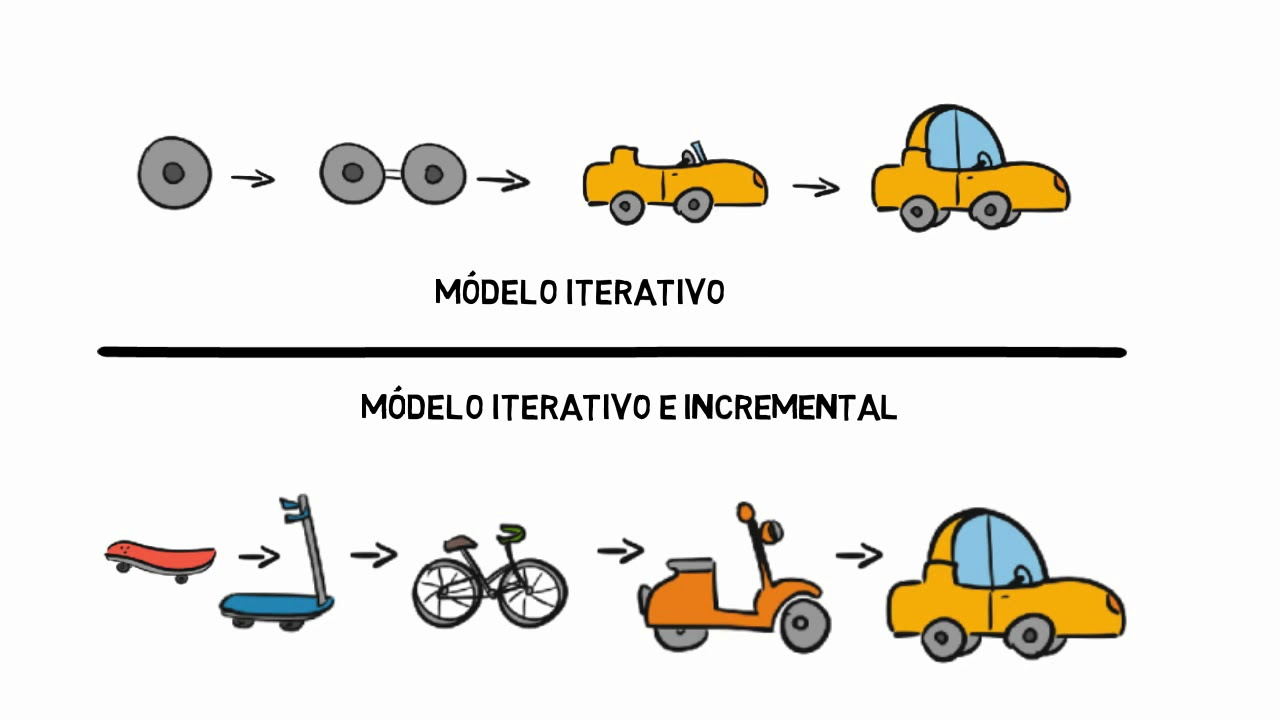
\includegraphics[width=0.7\textwidth, height = 6cm]{img/chapter03/iterativo incremental.jpg}
    \caption{Representación del modelo iterativo y modelo iterativo e incremental}
    \label{fig:iterativo_incremental}
\end{figure}

\textit{\textbf{Fase Preliminar:}} Diseño y Planificación (Iteración 0)
\begin{itemize}
    \item \textbf{Definición Detallada de Experimentos:} Elaboración de protocolos experimentales para los cuatro experimentos seleccionados (Reloj de Yodo, Sol de Fósforo, Síntesis de Cloruro de Amonio, Reacción Bromo-Aluminio), especificando reactivos, cantidades, procedimientos y resultados esperados.
    \item \textbf{Configuración del Entorno de Desarrollo:} Instalación y configuración de Unity (motor de videojuego), Blender (modelado 3D), Gimp (edición de imágenes) y entorno de programación C\#. Familiarización con las herramientas.
    \item \textbf{Definición del Alcance del Proyecto:} Establecimiento preciso de objetivos, funcionalidades, público objetivo, restricciones y plataforma de destino (Oculus Quest 2 y Meta Quest Pro).
    \item \textbf{Integración del SDK de Oculus:} Configuración del proyecto Unity para realidad virtual, integración del SDK de Oculus y pruebas de compatibilidad iniciales.
    \item \textbf{Implementación Básica del Seguimiento de Manos:} Habilitación y configuración inicial del sistema de seguimiento de manos en Unity, con pruebas preliminares de interacción
\end{itemize}

\textit{\textbf{Iteración 1:}} Base del Simulador y Tabla Periódica Interactiva
\begin{itemize}
    \item\textbf{Desarrollo del Entorno Virtual:} Creación del escenario del laboratorio y configuración de iluminación y ambiente.
    \item\textbf{Tabla Periódica Interactiva:} Diseño e implementación de una interfaz de tabla periódica funcional, con selección de elementos, visualización de información básica (nombre, símbolo, número atómico, masa atómica) y modelos 3D interactivos de isótopos.
    \item\textbf{Modelado 3D de Isótopos:} Diseño y creación de modelos 3D de los isótopos principales de cada elemento.
    \item\textbf{Integración de Modelos 3D:} Importación y configuración de los modelos 3D en Unity, estableciendo la conexión con la tabla periódica interactiva.
    \item\textbf{Modelado de Materiales y Herramientas:} Diseño y modelado 3D de materiales y herramientas de laboratorio (matraces, tubos de ensayo, mecheros, etc.) con funcionalidad básica de manipulación.
\end{itemize}

\textit{\textbf{Iteración 2:}} Tutorial Interactivo
\begin{itemize}
    \item \textbf{Diseño del Tutorial:} Elaboración de un guion detallado con objetivos de aprendizaje, pasos secuenciales e interacciones del usuario. Diseño de elementos visuales (flechas, indicaciones, animaciones) para guiar al usuario.
    \item \textbf{Implementación del Tutorial:} Programación de la lógica del tutorial en Unity, incluyendo instrucciones de voz (grabadas) y manejo de interacciones con objetos virtuales.
    \item \textbf{Pruebas y Ajustes:} Evaluación del tutorial con usuarios, realizando ajustes en base a la retroalimentación recibida para garantizar claridad, eficacia y usabilidad.
\end{itemize}
\newpage
\textit{\textbf{Iteraciones 3-6:}} Desarrollo de Experimentos
Para cada uno de los cuatro experimentos (De Básico a Ácido, La lampara de magnesio, Nieve Química, La Bruja de Bromo), se seguirá el siguiente proceso iterativo:
\begin{itemize}
    \item \textbf{Modelado 3D:} Creación de modelos detallados de reactivos y productos específicos del experimento.
    \item \textbf{Animaciones:} Desarrollo de animaciones realistas para representar las reacciones químicas y los cambios físicos observados.
    \item \textbf{Lógica del Experimento:} Implementación de la secuencia de pasos guiados, simulación de reacciones químicas (incluyendo cálculos de concentraciones, tiempos de reacción y cambios de color), evaluación formativa del desempeño del usuario y retroalimentación detallada.
    \item \textbf{Pruebas:} Pruebas del experimento para asegurar la precisión científica, la funcionalidad y la usabilidad.
\end{itemize}

\begin{figure}[thbp]
    \centering
    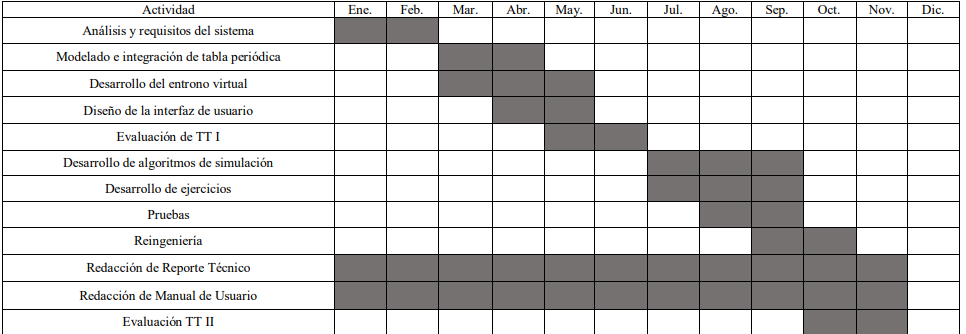
\includegraphics[width=0.8\textwidth, height = 7.5cm]{img/chapter03/Cronograma.png}
    \caption{Cronograma de Actividades}
    \label{fig:Cronograma}
\end{figure}

\section{Análisis de Requerimientos}
\subsection{Requerimientos Funcionales}
\begin{enumerate}[RF1.]
    \item \textit{Menú Principal: }El sistema presentará un menú principal intuitivo y organizado al inicio de la ejecución. Este menú proporcionará acceso a las funcionalidades del sistema, incluyendo un tutorial, selección de experimentos.
    \item \textit{Selección de Elementos}
    \begin{enumerate}[{RF2.}1.]
        \item \textit{Tabla Periódica Interactiva: }El sistema incorporará una tabla periódica interactiva que permita al usuario visualizar todos los elementos químicos de forma organizada.
        \item \textit{Selección Visual de Elementos: }El usuario podrá seleccionar elementos directamente desde la tabla periódica interactiva con un toque. 
        \item \textit{Visualización de Información Detallada: }Al seleccionar un elemento, se mostrará una ventana emergente con información detallada sobre el mismo, incluyendo su modelo atómico en 3D, descripción química y propiedades físicas y químicas. 
    \end{enumerate}
    \item \textit{Experimentación Virtual}
    \begin{enumerate}[{RF3.}1.]
        \item \textit{Instrucciones Paso a Paso:} El sistema guiará al usuario a través de cada experimento mediante instrucciones claras y concisas que detallen la cantidad de reactivos a utilizar y el procedimiento a seguir.
        \item \textit{Simulación de Reacciones: }El sistema simulará la reacción química entre los elementos seleccionados, siguiendo principios químicos establecidos.
        \item \textit{Observación de Efectos:} El usuario podrá observar los efectos de la reacción química en el entorno virtual, como la formación de nuevos compuestos, la liberación de gases o cambios de color.
    \end{enumerate}
\end{enumerate}
\subsection{Requerimentos No Funcionales}
\begin{enumerate}[RNF1.]
    \item \textit{Rendimiento}
    \begin{enumerate}[{RNF1.}1.]
        \item \textit{Fluidez Gráfica: }El sistema debe exhibir una tasa de cuadros por segundo (FPS) constante y superior a 60 FPS, para garantizar una experiencia de usuario inmersiva y sin interrupciones.
        \item \textit{Tiempo de Respuesta: }El sistema debe presentar un tiempo de respuesta mínimo a las acciones del usuario, minimizando los retrasos y garantizando una interacción dinámica y receptiva.
    \end{enumerate}
    \item \textit{Usabilidad}
    \begin{enumerate}[{RNF2.}1.]
        \item \textit{Interfaz Intuitiva: }La interfaz de usuario debe seguir principios de diseño intuitivos y accesibles, utilizando elementos visuales claros, jerarquías de información bien definidas y una navegación sencilla. 
        \item \textit{Navegación Sencilla: }La interfaz de usuario debe seguir principios de diseño intuitivos y accesibles, utilizando elementos visuales claros, jerarquías de información bien definidas y una navegación sencilla. 
        \item \textit{Retroalimentación Clara: }El sistema debe proporcionar retroalimentación clara y concisa al usuario sobre sus acciones e interacciones dentro del entorno virtual. 
    \end{enumerate}
\end{enumerate}
\newpage
\subsection{Reglas de Negocio}
El prototipo de simulador de laboratorio de química inorgánica en realidad virtual se regirá por las siguientes reglas de negocio: 

\begin{enumerate}[{RN-}01. ]
    \item \textit{\textbf{Selección de Elementos: }}
    \begin{itemize}
        \item Un elemento químico se considera seleccionado cuando el usuario toca su ficha en la tabla periódica con su dedo índice. 
        \item Solo se puede seleccionar un elemento a la vez. Si se selecciona un elemento que ya existe en la escena, este se destruye y se crea uno nuevo en la zona designada. 
        \item La GUI se actualizará con la información del elemento seleccionado. 
    \end{itemize}

    \item \textit{\textbf{Creación de Compuestos: }}
    \begin{itemize}
        \item Para crear un compuesto, el usuario debe llevar los elementos necesarios a la zona de creación. 
        \item El sistema verificará si cada elemento es correcto para el compuesto en dos ocasiones: al seleccionarlo y al entrar en la zona de creación. 
        \item Si un elemento es incorrecto, el sistema notificará al usuario mediante un mensaje de voz y texto, y le indicará que lo lleve a la zona de desecho. 
        \item El compuesto se formará solo cuando todos los elementos necesarios estén presentes en la zona de creación. 
        \item Una vez creado el compuesto, se mostrará su modelo 3D en el área de experimentación y se actualizará la GUI correspondiente. 
    \end{itemize}

    \item \textit{\textbf{Interacción con Objetos: }}
    \begin{itemize}
        \item El usuario puede agarrar, mover y soltar compuestos, instrumental y elementos utilizando el seguimiento de manos (hand tracking). 
        \item La interacción con objetos estará limitada a las acciones permitidas en cada etapa del experimento. 
    \end{itemize}

    \item \textit{\textbf{Simulación de Reacciones: }}
    \begin{itemize}
        \item La simulación de reacciones químicas presentará efectos visuales básicos, como cambios de color y liberación de gases, priorizando la comprensión de los conceptos fundamentales sobre el realismo detallado.
    \end{itemize}
    
    \item \textit{\textbf{Etapas del Experimento: }}
    \begin{itemize}
        \item Cada experimento se dividirá en cinco etapas: presentación, balanceo de ecuación, selección de elementos y creación de compuestos, desarrollo y simulación, y explicación de resultados y conclusiones. 
        \item El usuario avanzará a la siguiente etapa solo después de completar exitosamente la etapa anterior. 
        \item En la etapa de desarrollo y simulación, el usuario seguirá instrucciones paso a paso y realizará las acciones necesarias para completar el experimento. 
    \end{itemize}
    \newpage
    \item \textit{\textbf{Retroalimentación al Usuario: }}
    \begin{itemize}
        \item El sistema proporcionará retroalimentación visual y auditiva al usuario en cada etapa del experimento. 
        \item En caso de errores, se mostrarán mensajes claros y concisos en la GUI indicando el problema y cómo solucionarlo. 
    \end{itemize}
    
    \item \textit{\textbf{Navegación:}}  
    \begin{itemize}
        \item Al finalizar un experimento, el usuario será redirigido automáticamente al escenario de bienvenida. 
        \item Desde el escenario de bienvenida, el usuario podrá seleccionar otro experimento o repetir el tutorial.
    \end{itemize}

    \item \textit{\textbf{Eliminación de Elementos: }}
    \begin{itemize}
        \item Los elementos químicos y compuestos pueden ser eliminados del área de trabajo arrastrándolos a la zona de desecho. 
        \item El sistema verificará si el elemento o compuesto puede ser desechado en ese momento del experimento. 
    \end{itemize}

    \item \textit{\textbf{Balanceo de Ecuaciones:}} 
    \begin{itemize}
        \item En la etapa de balanceo de ecuaciones, el usuario deberá ajustar los coeficientes estequiométricos de la reacción química para cumplir con la ley de conservación de la masa.   
        \item El sistema verificará si la ecuación está correctamente balanceada antes de permitir al usuario avanzar a la siguiente etapa. 
    \end{itemize}
    \item \textit{\textbf{Tutorial Interactivo: }}
    \begin{itemize}
        \item El tutorial guiará al usuario a través de las funciones básicas del simulador, incluyendo la selección de elementos, la creación de compuestos y la interacción con el instrumental. 
        \item El tutorial será opcional y podrá ser repetido en cualquier momento desde el menú principal. 
    \end{itemize}
\end{enumerate}

\subsection{¿Como debe venderse?}
Como una herramienta educativa y de entretenimiento inmersiva que permite a los usuarios explorar y experimentar con la química inorgánica de manera segura y divertida. El simulador ofrece una experiencia interactiva y visualmente atractiva, que permite a los usuarios manipular elementos químicos, realizar experimentos guiados y observar reacciones en tiempo real en un entorno de laboratorio virtual. 

Se puede distribuir de dos formas: 
\begin{itemize}
    \item\textit{\textbf{Versión demo gratuita:}} permitiendo a los usuarios potenciales experimentar con una selección limitada de experimentos y familiarizarse con la interfaz y el funcionamiento del simulador. 
    \item\textit{\textbf{Licencia completa:}} proporcionando acceso completo a todas las funcionalidades y experimentos disponibles en el simulador. 
\end{itemize}

El público objetivo del simulador incluye: 
\begin{itemize}
    \item Estudiantes de secundaria y nivel medio superior que cursan química. 
    \item Profesores de química que buscan herramientas innovadoras para sus clases. 
    \item Aficionados a la ciencia y entusiastas de la realidad virtual. 
    \item Museos y centros de ciencia que buscan ofrecer experiencias educativas interactivas. virtual.
\end{itemize}
\subsection{Limitaciones del Sistema}
El prototipo de simulador de laboratorio de química inorgánica en realidad virtual presentará las siguientes limitaciones inherentes a su diseño y alcance: 

\begin{itemize}
    \item \textbf{Ámbito Exclusivo en Química Inorgánica:} El simulador se circunscribe a la simulación de experimentos dentro del dominio de la química inorgánica, excluyendo otras ramas de la química, como la orgánica, la bioquímica o la fisicoquímica. 
    \item \textbf{Experimentación Guiada y Estructurada:} La experiencia del usuario se centra en experimentos predefinidos y guiados, priorizando la facilidad de uso y la comprensión de los conceptos fundamentales de la química inorgánica. No se contempla la posibilidad de realizar experimentos libres o personalizados en esta versión.

    \item \textbf{Limitaciones en el Realismo:} Aunque se busca la mayor fidelidad posible a la realidad, es importante destacar que el simulador ofrece una representación virtual de los fenómenos químicos. Algunas reacciones o propiedades químicas podrían ser simplificadas o idealizadas para facilitar la comprensión y el uso educativo, sin comprometer la validez de los conceptos aprendidos.
    \item \textbf{Plataformas Compatibles:} El simulador será compatible exclusivamente con los dispositivos de realidad virtual Oculus Meta Quest 2 y Oculus Meta Quest Pro. 
\end{itemize}
\newpage
\section{Tecnologías de Desarrollo}
\subsection{Modelado 3D y Animación}
\subsubsection{Blender}\\

Blender 3D es un software multiplataforma y gratuito especializado en el modelado, iluminación, renderizado, animación y creación de modelos 3D. También incluye composición digital utilizando nodos, edición de video, escultura y pintura digital.

El objetivo principal de Blender es generar imágenes 2D a partir de escenas 3D, utilizando diversos motores gráficos, tanto de pre-renderizado como de tiempo real, que vienen integrados por defecto. El programa ofrece una variedad de figuras geométricas primitivas, como curvas, mallas poligonales, vacíos y metaballs, además de una amplia gama de herramientas para modelado, renderizado, rigging, edición de video, audio, composición y animación.

Blender también incluye herramientas de animación avanzadas como cinemática inversa, deformaciones con armaduras o cuadrículas, vértices de carga y partículas estáticas. Además, proporciona características interactivas para el desarrollo de juegos, incluyendo detección de colisiones, simulaciones dinámicas, aplicación de físicas y lógica.

La interfaz gráfica OpenGL de Blender es uniforme y personalizable en las principales plataformas, y permite el uso de scripts en Python para automatizar y controlar varias tareas. Admite formatos gráficos como TGA, JPG, Iris, SGI y TIFF, e incluye simulaciones dinámicas para cuerpos blandos, partículas y fluidos. También cuenta con un sistema de partículas estáticas para simular cabello y pelaje, con opciones avanzadas de shaders para texturas realistas.

Desde su creación en 2001, Blender ha sido reconocido por su constante desarrollo y mejoras, proporcionando a los usuarios una experiencia única y en evolución.\\

\begin{figure}[thbp]
    \centering
    \includegraphics[width=0.5\textwidth, height = 5cm]{img/chapter03/Modelo_Atómico.png}
    \caption{Modelo de un átomo en Blender}
    \label{fig:atomo}
\end{figure}

\subsubsection{Gimp}
Este software de manipulación de imágenes ha experimentado una notable evolución a lo largo del tiempo. Utiliza GTK como biblioteca de controles gráficos.

Permite trabajar con imágenes en capas, lo que facilita la modificación independiente de cada objeto en la imagen. Las capas pueden organizarse en una pila, subiendo o bajando de nivel para facilitar la edición. Cada capa tiene su propia visibilidad y nivel de transparencia, y hay numerosas formas de combinar las relaciones entre ellas.

Además, es posible producir imágenes de manera completamente automatizada y no interactiva, así como realizar un procesamiento por lotes que cambia colores o convierte series de imágenes. Para tareas automatizadas más simples, se recomienda utilizar un paquete como ImageMagick.

\textit{\textbf{Imágenes}}\\
Una imagen en GIMP puede ser más compleja de lo que parece. No es solo un dibujo en un lienzo, sino una pila de capas, una máscara de selección, un conjunto de canales y rutas.

Cuenta con un sistema de gestión de memoria avanzado basado en bloques de píxeles, lo que permite manejar imágenes muy grandes sin dificultad.

\textit{\textbf{Capas}}\\
Una imagen con capas es similar a un fajo de papeles transparentes apilados. Se puede dibujar en cada papel y ver el contenido de otras hojas a través de las áreas transparentes. También es posible mover una hoja en relación con las demás.

Una imagen en GIMP puede contener muchas capas, incluso docenas. Las capas no tienen que ser opacas ni cubrir toda la extensión de la imagen, por lo que se puede ver más que la capa superior, observando elementos de otras capas.

\textit{\textbf{Canales}}\\
Los canales son útiles cuando se trabaja en una imagen que necesita ajustes en un color específico. Ver los canales como máscaras permite restringir la salida del color que el canal representa. Usando filtros en la información del canal, se pueden crear muchos efectos variados y sutiles sobre una imagen. Con estos canales, es posible crear otros canales, conocidos como máscaras de canal.
\subsection{Motor de Videojuegos}
\subsubsection{Unity}
Unity es una plataforma líder en el desarrollo de juegos, compatible con múltiples plataformas, ampliamente utilizada para crear experiencias interactivas tanto en 3D como en 2D. Su ecosistema completo, que incluye un amplio conjunto de herramientas y una comunidad activa, facilita la creación de simulaciones de realidad virtual realistas, la interacción natural con elementos virtuales y el desarrollo de interfaces de usuario intuitivas.

El entorno integrado de Unity está compuesto por diversas partes y componentes que permiten el desarrollo de simuladores. Está desarrollado en C\#, un lenguaje de programación multiparadigma que, al ser de acceso libre, fomenta la creación de contenido por parte de la comunidad y la creación de sus propias librerías.

C\# es la tercera versión de C y una mejora respecto a C++, lo que simplifica la exportación y comunicación con programas escritos en estos lenguajes sin necesidad de una interfaz compleja.

\subsubsection{C\#}
C\# es un lenguaje de programación que se centra en componentes, está orientado a objetos y garantiza la seguridad de tipos. Esto permite a los desarrolladores crear una variedad de aplicaciones seguras y robustas que se ejecutan en el entorno .NET. Es especialmente adecuado para la creación y utilización de componentes de software, y ofrece características que respaldan nuevas cargas de trabajo y prácticas de diseño de software en evolución. En esencia, C\#  es un lenguaje orientado a objetos.

\subsubsection{GameObject}
Los GameObject son elementos esenciales en Unity, ya que pueden representar diversos elementos como avatares, objetos o el escenario mismo. Por sí solos, estos elementos no realizan ninguna función, pero actúan como contenedores para sus Componentes.

\begin{figure}[thbp]
    \centering
    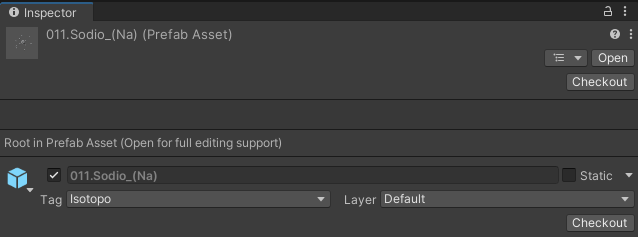
\includegraphics[width=0.7\textwidth, height = 4cm]{img/chapter03/Game_Object.png}
    \caption{Game Object en Unity}
    \label{fig:game_object}
\end{figure}

\subsubsection{Componentes}
Los componentes son los que definen el comportamiento de cada GameObject en el juego. No existe un límite establecido en cuanto a la cantidad de componentes que puede tener un objeto.

\begin{figure}[thbp]
    \centering
    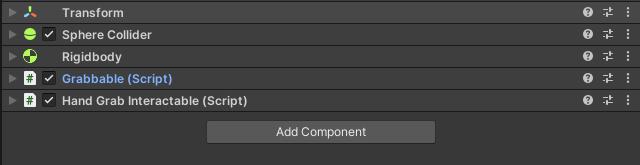
\includegraphics[width=0.7\textwidth, height = 4cm]{img/chapter03/Components.png}
    \caption{Componentes de un Elemento en Unity}
    \label{fig:components}
\end{figure}

\subsubsection{Script}
El Script es un componente diseñado por el usuario para realizar una acción específica en el juego. Consiste en una secuencia de líneas de comandos escritas principalmente en C\# o en UnityScript. Sin embargo, otros lenguajes .NET pueden ser utilizados con Unity si son compilados en un DLL compatible.

Los Scripts permiten activar eventos en su juego, modificar propiedades del Componente en tiempo real y responder al input del usuario de la manera que desee. Puede crear un nuevo script desde el menú ``Create'' en la parte superior izquierda del panel del Proyecto, o seleccionando ""Assets \verb|>| Create \verb|>| C\# Script"" desde el menú principal.

Cuando se adjunta un componente script a un GameObject, se crea una nueva instancia del objeto definido por el plano. Es importante tener en cuenta que un script solo define un plano para un componente; su código no se activará hasta que una instancia del script sea adjuntada al GameObject.

\subsubsection{ScriptableObject}
ScriptableObject es una clase en Unity que permite almacenar grandes cantidades de datos compartidos independientes de las instancias de script. A diferencia de SerializableObject, esta clase está diseñada específicamente para este propósito y no debe confundirse con ella.

Cuando se utiliza ScriptableObject, los datos se almacenan por referencia en lugar de por valor, lo que significa que las instancias de ScriptableObject mantienen los datos y las instancias de script solo contienen referencias a estos datos. Esto ayuda a reducir el uso de memoria al evitar la duplicación de valores.

Un caso de uso común para ScriptableObject es definir conjuntos de datos conectables, como en el caso de una tienda NPC en un juego RPG, donde cada zona puede ofrecer diferentes tipos de ítems para la venta. Los objetos de ScriptableObject personalizados pueden definir estos conjuntos de datos, lo que permite una fácil configuración y personalización del juego.
\begin{figure}[thbp]
    \centering
    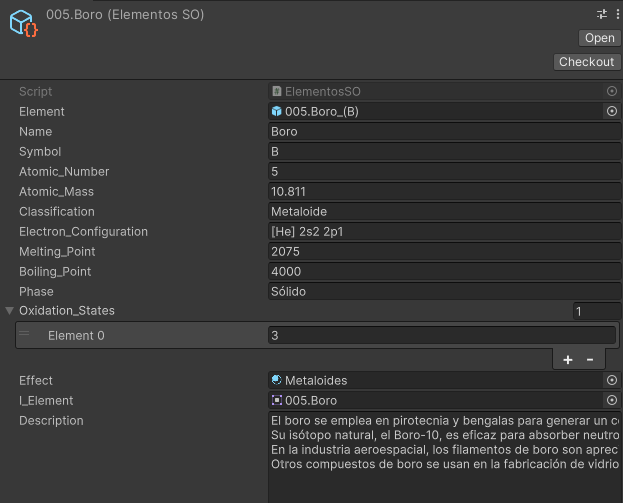
\includegraphics[width=0.6\textwidth, height = 7cm]{img/chapter03/ScriptableObject.png}
    \caption{ScriptableObject de un Elemento en Unity}
    \label{fig:components}
\end{figure}
\newpage
\subsection{Integración de Oculus Meta Quest 2 y Oculus Meta Quest Pro}
Meta Quest 2 y Meta Quest Pro son dispositivos de realidad virtual (VR) desarrollados por Meta Platforms (anteriormente Facebook), cada uno diseñado para satisfacer necesidades y expectativas específicas de los usuarios.

\textit{Meta Quest 2:} Lanzado en 2020, este dispositivo autónomo ofrece una experiencia de VR inmersiva sin necesidad de una PC externa, proporcionando un rendimiento fluido en la mayoría de aplicaciones y juegos disponibles en su plataforma, brindando una experiencia visual de alta calidad.

\begin{figure}[thbp]
    \centering
    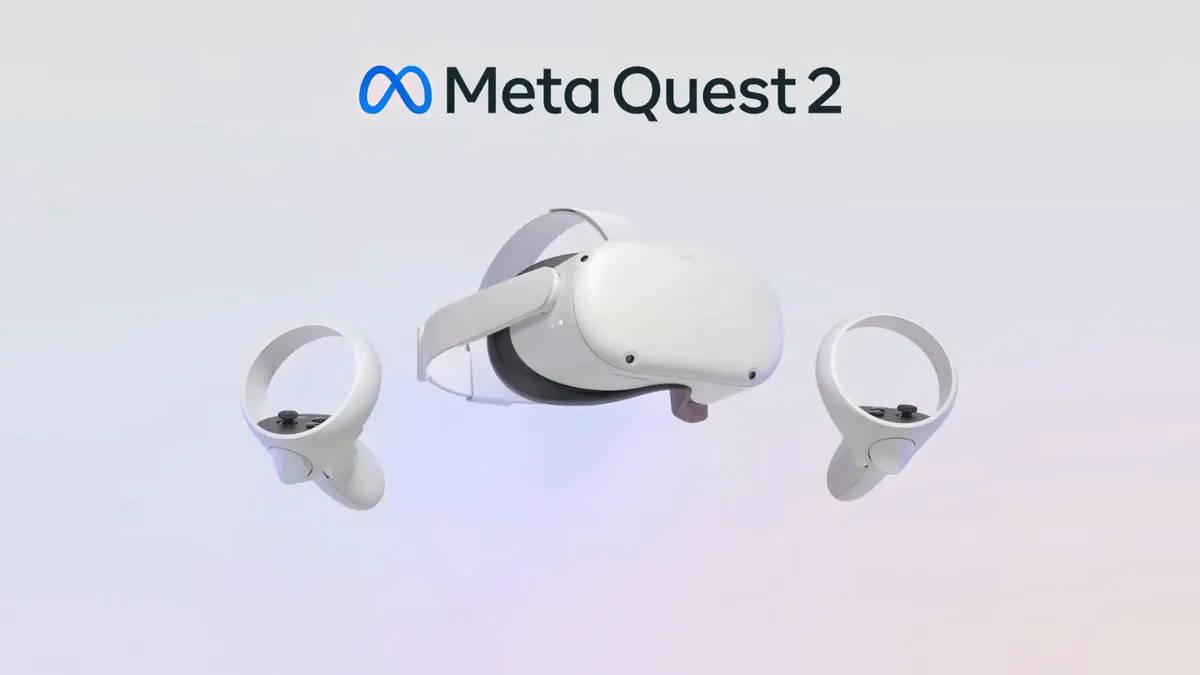
\includegraphics[width=0.5\textwidth, height = 4cm]{img/chapter03/Meta_Quest_2.png}
    \caption{Oculus Meta Quest 2}
    \label{fig:Oculus_Meta_Quest_2}
\end{figure}

\textit{Meta Quest Pro:} Lanzado en 2022, este dispositivo de gama alta está orientado a profesionales y entusiastas de la VR, ofrece un rendimiento superior y capacidades avanzadas. Además, incorpora seguimiento ocular y facial, así como cámaras de alta resolución, que permiten una interacción más natural y expresiva en entornos virtuales, y habilitan funciones de realidad mixta.

\begin{figure}[thbp]
    \centering
    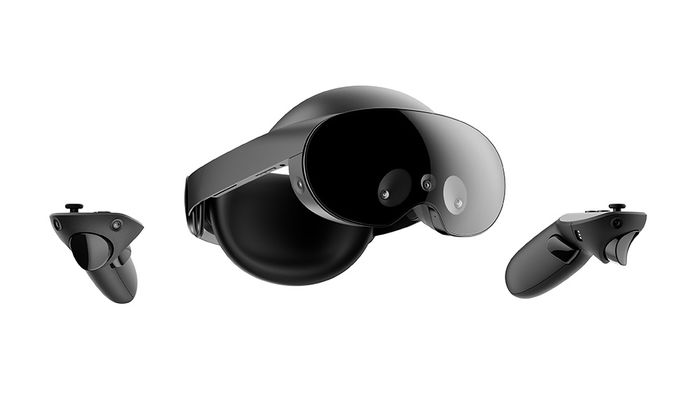
\includegraphics[width=0.5\textwidth, height = 4cm]{img/chapter03/Meta_Quest_Pro.png}
    \caption{Oculus Meta Quest Pro}
    \label{fig:Oculus_Meta_Quest_Pro}
\end{figure}

\textit{SDK de Oculus}

El SDK de Oculus proporciona las herramientas y bibliotecas necesarias para integrar el simulador con las gafas VR Oculus Meta Quest 2 y Oculus Meta Quest Pro de manera nativa. Permite el seguimiento preciso de la cabeza y el movimiento de las manos, la representación 3D estereoscópica de alta calidad y la interacción natural con elementos virtuales, creando una experiencia de realidad virtual inmersiva y atractiva.

\begin{longtable}{|>{\centering\arraybackslash}m{.2\textwidth}|>{\centering\arraybackslash}m{.4\textwidth}|>{\centering\arraybackslash}m{.4\textwidth}|}
    \hline
    \rowcolor{blue_escom}
    Característica & Meta Quest 2 & Meta Quest Pro  \\
    \hline
    \endfirsthead

    \hline
    \rowcolor{blue_escom}
    Característica & Meta Quest 2 & Meta Quest Pro  \\
    \hline
    \endhead

    \multicolumn{3}{r}{\textit{Continúa en la siguiente página}} \\
    \endfoot

    \endlastfoot

    \cellcolor{column_color}Resolución por Ojo & 1832x1920 pixeles & 1800x1920 pixeles \\
    \hline
    \cellcolor{column_color}Frecuencia de Actualizaión & 72-90 Hz & 72-90 Hz \\
    \hline
    \cellcolor{column_color}Procesador & Qualcomm Snapdragon XR2 & Qualcomm Snapdragon XR2+ \\
    \hline
    \cellcolor{column_color}RAM & 6 GB & 12 GB \\
    \hline
    \cellcolor{column_color}Almacenamiento & 128 GB / 256 GB & 256 GB \\
    \hline
    \cellcolor{column_color}Seguimiento Ocular y Facial & ✗ & ✓ \\
    \hline
    \cellcolor{column_color}Cámaras & 4 & 10 \\
    \hline
    \cellcolor{column_color}Realidad Mixta & ✗ & ✓ \\
    \hline
    \cellcolor{column_color}Duración de la batería & 2-3 horas & 2-3 horas \\
    \hline
    \cellcolor{column_color}Precio aproximado & \$299 USD (128 GB) / \$399 USD (256 GB) & \$999 USD \\
    \hline

  \caption{Comparación de especificaciones entre Oculus Meta Quest 2 y Oculus Meta Quest Pro}
  \label{tab:Quest_2_vs_Quest_Pro}
\end{longtable}
\newpage
\subsection{Handtracking}
El seguimiento de manos (hand tracking) es una tecnología que permite la detección y seguimiento en tiempo real de los movimientos de las manos del usuario a través de dispositivos equipados con cámaras, como las gafas de realidad virtual Meta Quest. Esta tecnología se basa en el análisis de imágenes capturadas por las cámaras, identificando puntos clave en las manos y rastreando su movimiento a medida que el usuario las desplaza.
El seguimiento de manos ofrece una modalidad de interacción más natural e intuitiva con dispositivos y entornos virtuales, eliminando la necesidad de controladores físicos.

\textbf{En Realidad virtual (VR) y realidad mixta:} Permite una interacción más inmersiva y realista con entornos virtuales, mejorando la experiencia del usuario en juegos, simulaciones y aplicaciones de entrenamiento.\\
\begin{figure}[thbp]
    \centering
    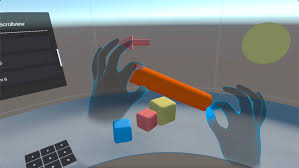
\includegraphics[width=0.5\textwidth, height = 4cm]{img/chapter03/hand_tracking.jpeg}
    \caption{Ejemplo de Handtracking}
    \label{fig:Handtracking}
\end{figure}
\section{Análisis Económico}
\subsection{Análisis por Puntos de Función}
Métrica de punto de función La métrica de punto de función (PF) puede usarse de manera efectiva como medio para medir la funcionalidad que entra a un sistema. 

Para obtener el PF vamos a considerar los valores de dominio de información que se definen de la siguiente forma:  

\textit{\textbf{Número de entradas externas (EE): 5}}
\begin{itemize}
    \item Elegir experimento/tutorial (Simple)
    \item Seleccionar elemento (Simple)
    \item Eliminar elemento (Simple) 
    \item Crear compuesto (Simple) 
    \item Interactuar con instrumental (Simple)
\end{itemize}
\textit{\textbf{Número de salidas externas (SE): 3  }}
\begin{itemize}
    \item Visualización del experimento (Complejo)
    \item Resultados del experimento (Complejo)
    \item Visualización del Entorno de Laboratorio (Promedio)
    \item Visualización de Elementos y Compuestos (Promedio)
    \item Indicaciones visuales y auditivas (Promedio) 
\end{itemize}
\textit{\textbf{Número de consultas externas (CE): 0  }}

\textit{\textbf{Número de archivos lógicos internos (ALI): 3  }}
\begin{itemize}
    \item Datos de experimentos (Promedio)
    \item Datos de elementos (Promedio)
    \item Datos de compuestos (Promedio)
\end{itemize}
\textit{\textbf{Número de archivos de interfaz externos (AIE): 0  }}

\begin{table}[H]
  \centering
  \begin{tabular}{|>{\centering\arraybackslash}m{.2\textwidth}|>{\centering\arraybackslash}m{.13\textwidth}>
  {\centering\arraybackslash}m{.015\textwidth}>{\centering\arraybackslash}m{.095\textwidth}>{\centering\arraybackslash}m{.095\textwidth}>{\centering\arraybackslash}m{.095\textwidth}>{\centering\arraybackslash}m{.015\textwidth}>{\centering\arraybackslash}m{.07\textwidth}|}
    \hline
    \rowcolor{blue_escom}
     &\multicolumn{7}{c|}{\parbox[0.53\textwidth]{0.515\textwidth}{\centering\textbf{Factor Ponderado}}}\\
    \cline{2-8} 
    
    \multirow{-2}{.2\textwidth}{\cellcolor{blue_escom} \centering \textbf{Valor de dominio de información}} & Conteo & & Simple & Promedio & Complejo & & Total\\ 
    \hline
    \cellcolor{column_color}Entradas Externas (EE) & 5 Simples & * & 3 & 4 & 6 & = & 15 \\
    \hline
    \cellcolor{column_color}Salidas Externas (SE) & 2 Complejos, 3 Promedio & * & 4 & 5 & 7 & = & 29 \\
    \hline
    \cellcolor{column_color}Consultas Externas (CE) & 0 & * & 3 & 4 & 6 & = & 0 \\
    \hline
    \cellcolor{column_color}Archivos Lógicos Internos (ALI) & 3 Promedios & * & 7 & 10 & 15 & = & 30 \\
    \hline
    \cellcolor{column_color}Archivos de Interfaz Externos (AIE) & 0 & * & 5 & 7 & 10 & = & 0 \\
    \hline
    \cellcolor{column_color}Conteo Total & & & & & & & \cellcolor{column_color}74 \\
    \hline
  \end{tabular}
  \caption{Cálculo de Puntos de Función (PF)}
  \label{tab:Cálculo_de_Puntos_de_Función_(PF)}
\end{table}
\newpage
Una vez obtenido lo anterior continuaremos con la obtención de los Fi (i = 1 a 14) son factores de ajuste de valor (FAV) con base en respuestas a las siguientes preguntas cada una de estas preguntas se responde usando una escala que varía de 0 (no importante o aplicable) a 5 (absolutamente esencial).  

\begin{enumerate}
    \item \textit{\textbf{¿Requiere el sistema copias de seguridad y recuperación fiables?}} 0 no influye en el sistema. 
    \item \textit{\textbf{¿Se requiere comunicación de datos?}} 0 no influye en el sistema.     
    \item \textit{\textbf{¿Existen funciones de procesamiento distribuido?}} 0 no influye en el sistema.     
    \item \textit{\textbf{¿Es crítico el rendimiento?}} 5 es absolutamente escencial     
    \item \textit{\textbf{¿Se ejecutará en un entorno operativo existente y fuertemente utilizado?}} 2 de moderada importancia     
    \item \textit{\textbf{¿Requiere entrada de datos interactiva?}} 5 es absolutamente escencial     
    \item \textit{\textbf{¿Requiere la entrada interactiva transacciones en múltiples pantallas?}} 0 no influye en el sistema.     
    \item \textit{\textbf{¿Se actualizan los archivos maestros de forma interactiva?}} 2 de moderada importancia     
    \item \textit{\textbf{¿Son complejas las entradas, salidas, archivos o consultas?}} 4 significativa importancia     
    \item \textit{\textbf{¿Es complejo el procesamiento interno?}} 4 significativa importancia     
    \item \textit{\textbf{¿Se ha diseñado el código para ser reutilizable?}} 5 es absolutamente escencial  
    \item \textit{\textbf{¿Están incluidas en el diseño la conversión y la instalación?}} 1 de poca importancia     
    \item \textit{\textbf{¿Se ha diseñado para múltiples instalaciones en diferentes organizaciones?}} 2 de moderada importancia     
    \item \textit{\textbf{¿Se ha diseñado para facilitar cambios y ser fácil de usar?}} 4 significativa importancia 
\end{enumerate}

Una vez terminado de responder las preguntas realizamos las sumas de los $F_{i}:$
\[\Sigma (F_{i}) = 34\]

Teniendo ya estos datos podemos obtener los puntos de función utilizando la siguiente expresión  
\begin{center}
    \textit{\textbf{PF = Conteo Total }}$* (0.65 + 0.01 * \Sigma (F_{i}))$

    $PF = 74 * (0.65 + 0.01 * 34)$
    
    $PF = 73.26$
\end{center}
\newpage
\textit{\textbf{Estimación COCOMO}} 

El modelo COCOMO, desarrollado por Barry W. Boehm, estima la cantidad de meses-hombre necesarios para desarrollar un software. Consta de tres submodelos (orgánico, semiacoplado y empotrado) que varían en detalle y precisión. La elección del submodelo depende de la cantidad estimada de miles de líneas de código (KLDC), que se puede aproximar utilizando el factor de productividad (PF) obtenido previamente y la siguiente tabla de referencia.

\begin{figure}[thbp]
    \centering
    \includegraphics[width=1\textwidth]{img/chapter03/Tabla de lenguajes de puntos de función.png}
    \caption{Tabla de lenguajes de puntos de función - QSM\cite{QSM}}
    \label{fig:QSM}
\end{figure}

El lenguaje utilizado será C\#, que tiene un LOC promedio de 54 líneas por función. Con estos valores, se aplican a la siguiente fórmula para obtener una estimación en miles de líneas de código:

\begin{center}
    \textit{\textbf{KLDC} = (PF) $*$ (Promedio de líneas por función}

    \textit{\textbf{KLDC} = $73.26 * 54$}

    \textit{\textbf{KLDC} = $3,956.04$}
\end{center}

\textbf{KLDC = 3.9560 miles de líneas de código}

A continuación, se observa en cuál submodelo se clasificará el presente proyecto según los siguientes criterios:
\begin{itemize}
    \item Orgánico: Proyectos pequeños con menos de 50 KLCD
    \item Semiacoplado: Proyectos de complejidad media con menos de 300 KLCD
    \item Empotrado: Proyectos muy complejos donde no hay experiencia previa y se utiliza tecnología de vanguardia
\end{itemize}
Dado que el proyecto tiene menos de 50 KLCD, se clasifica en el submodelo Orgánico. Aunque todos los submodelos utilizan las mismas ecuaciones para la estimación, emplean diferentes coeficientes, los cuales se presentan en la siguiente tabla:

\begin{table}[H]
  \centering
  \begin{tabular}{|>{\centering\arraybackslash}m{.4\textwidth}|>{\centering\arraybackslash}m{.1\textwidth}>
  {\centering\arraybackslash}m{.1\textwidth}>
  {\centering\arraybackslash}m{.1\textwidth}>
  {\centering\arraybackslash}m{.1\textwidth}|}
    \hline
    \rowcolor{blue_escom}
     Proyecto de Software & a & b & c & d \\
    \hline
    Orgánico & 2.4 & 1.05 & 2.5 & 0.38 \\
    \hline
    Semiacoplado & 3.0 & 1.12 & 2.5 & 0.35 \\
    \hline
    Empotrado & 3.6 & 1.20 & 2.5 & 0.32 \\
    \hline
  \end{tabular}
  \caption{COCOMO básico}
  \label{tab:COCOMO}
\end{table}

Se procede a realizar el cálculo del esfuerzo por persona-mes. Siendo a y b coeficientes de la \autoref{tab:COCOMO}

\begin{center}
    \textit{\textbf{E} = a $*$ (KLDC)$^b$}

    \textit{\textbf{E} = $(2.4) * (3.9560)^1.05$}

    \textit{\textbf{E} = $10.17$ persona-mes}
\end{center}
A continuación, se calcula la duración del proyecto utilizando la siguiente fórmula:
\begin{center}
    \textit{\textbf{D} = c $*$ E$^d$}

    \textit{\textbf{D} = $(2.5) * (10.17021979)^{0.38}$}

    \textit{\textbf{D} = 6.035 meses}
\end{center}

Por lo que se puede observar los resultados arrojan que el tiempo en el que se debe desarrollar el proyecto es de 6 meses con 2 personas.

Por lo tanto, se concluye que la estimación del tiempo de desarrollo del proyecto es de 6 meses con 2 personas, lo que implica un esfuerzo de 12 meses-persona. Al considerar que el proyecto será desarrollado por una sola persona, la duración ajustada del proyecto se estima en aproximadamente 10 meses. Este tiempo es justo, pero no es tolerante a retrasos.

Es importante destacar que, al tener un margen de tiempo limitado para el desarrollo del proyecto, se presenta un riesgo moderado a significativo. Cualquier retraso en el cronograma puede afectar negativamente la implementación de algunas funcionalidades del sistema. 

\subsection{Análisis de costos}
El análisis de costos del sistema se basa en una lista detallada de todos los gastos asociados a su desarrollo.

El proyecto considera un total de 660 horas-hombre de desarrollo.

\textit{\textbf{Mano de obra}}

El costo de la mano de obra se calcula considerando un total de 660 horas-hombre, con un salario estimado de \$70.00 MXN por hora o \$11,200.00 MXN mensuales.

La distribución del tiempo de desarrollo y los costos asociados se detalla en la \autoref{tab:Desarrollo}:
\begin{table}[H]
  \centering
  \begin{tabular}{|>{\centering\arraybackslash}m{.3\textwidth}|>{\centering\arraybackslash}m{.3\textwidth}|>{\centering\arraybackslash}m{.2\textwidth}|}
    \hline
    \rowcolor{blue_escom}
     \textbf{Equipo} & \textbf{Costo} & \textbf{Tiempo}\\
     \hline
     Modelado 3D, 2D y VFX & \$11,550.00 & 165 hrs.\\
     Software & \$27,720.00 & 396 hrs.\\
     VR & \$6,930.00 & 99 hrs.\\
     \hline
     \rowcolor{column_color}
     \textbf{Total} & \$46,200.00 & 660 hrs.\\
     \hline
  \end{tabular}
  \caption{Costos de Desarrollo}
  \label{tab:Desarrollo}
\end{table}
\newpage
\textit{\textbf{Equipo de Desarrollo}}

El equipo de desarrollo incluye todos los recursos necesarios para diseñar y ejecutar el prototipo. Los componentes principales son:
\begin{itemize}
    \item Computadora de Desarrollo\\
    Se utilizará una laptop de gama media-alta para ejecutar el sistema.\\
    \textbf{MSI Katana 15 B12V:} \$25,440.00
    \begin{itemize}
        \item \textbf{Procesador:} Intel Core i7 12650H
        \item \textbf{Memoria RAM:} 16 GB DDR5
        \item \textbf{Almacenamiento:} 1 TB SSD
        \item \textbf{Tarjeta gráfica:} NVIDIA GeForce RTX 4070
        \item \textbf{Sistema operativo:} Windows 11\\
        \begin{figure}[thbp]
            \centering
            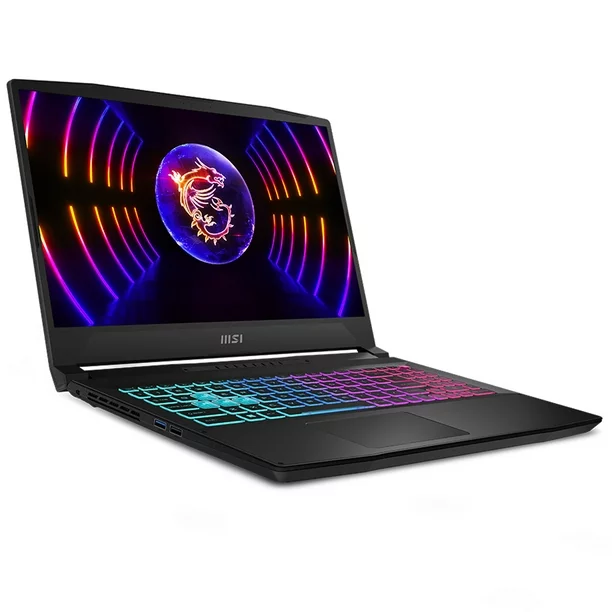
\includegraphics[width=0.5\textwidth, height = 7cm]{img/chapter03/MSI_KATANA.png}
            \caption{Laprop MSI Katana 15 B12V}
            \label{fig:MSI_Katana}
        \end{figure}
    \end{itemize}
\end{itemize}

\begin{itemize}
    \item Gafas de Realidad Virtual\\
    Se cuenta con las gafas Oculus Meta Quest Pro con un costo aproximado en México de \$20,000.00 MXN y las gafas Oculus Meta Quest 2 con un costo aproximado de \$10,000.00 MXN\\
    \begin{figure}[thbp]
        \centering
        \begin{subfigure}[b]{0.45\linewidth}
            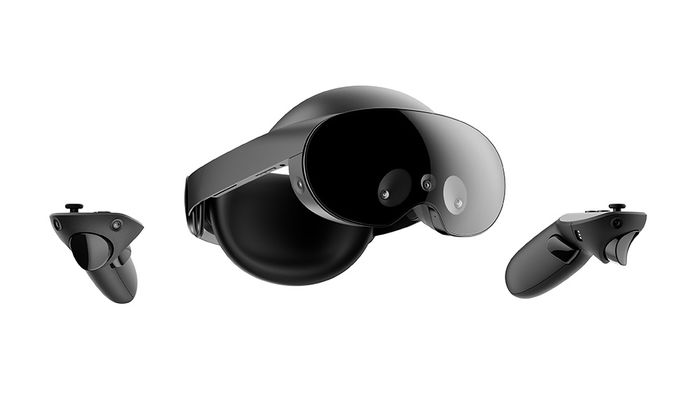
\includegraphics[width=\linewidth, height = 4cm]{img/chapter03/Meta_Quest_Pro.png}
            \caption{Oculus Meta Quest Pro}
            \label{fig:Oculus_Meta_Quest_Pro}
        \end{subfigure}
        \begin{subfigure}[b]{0.45\linewidth}
            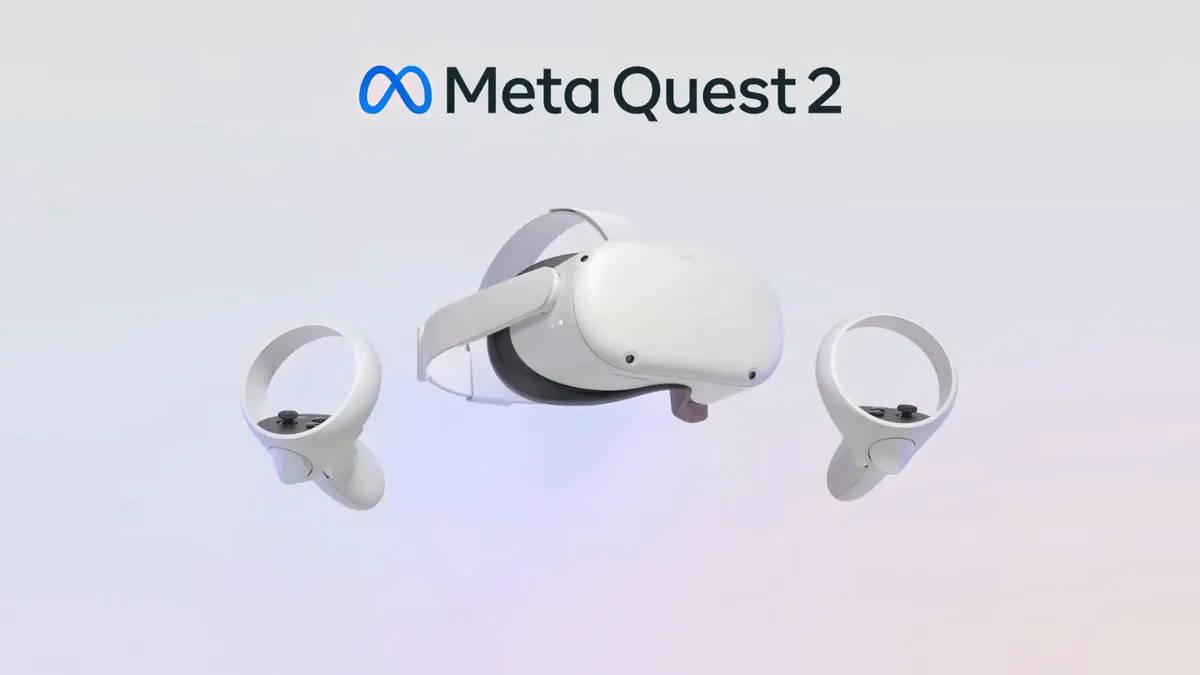
\includegraphics[width=\linewidth, height = 4cm]{img/chapter03/Meta_Quest_2.png}
            \caption{Oculus Meta Quest 2}
            \label{fig:Oculus_Meta_Quest_2}
        \end{subfigure}
        \caption{Sistemas Compatibles}
    \end{figure}
\end{itemize}

\begin{table}[H]
  \centering
  \begin{tabular}{|>{\centering\arraybackslash}m{.5\textwidth}|>{\centering\arraybackslash}m{.3\textwidth}|}
    \hline
    \rowcolor{blue_escom}
     \textbf{Objeto} & \textbf{Costo} \\
     \hline
     Laptop MSI Katana 15 B12V & \$25,440.00\\
     Oculus Meta Quest Pro & \$20,000.00\\
     Oculus Meta Quest 2 & \$10,000.00\\
     \hline
     \rowcolor{column_color}
     \textbf{Total} & \$55,440.00\\
     \hline
  \end{tabular}
  \caption{Costos de Infraestructura}
  \label{tab:Costos}
\end{table}

\textit{\textbf{Licenciamiento}}

Se incluyen las licencias y herramientas externas necesarias para el desarrollo, como se detalla en la \autoref{tab:Licencias}.
\begin{table}[H]
  \centering
  \begin{tabular}{|>{\centering\arraybackslash}m{.5\textwidth}|>{\centering\arraybackslash}m{.3\textwidth}|}
    \hline
    \rowcolor{blue_escom}
     \textbf{Licenciamiento} & \textbf{Costo}\\
     \hline
     Unity Assets & \$5,000.00\\
     SPEECHGEN.IO & \$600.00\\
     3D & \$500.00\\
     \hline
     \rowcolor{column_color}
     \textbf{Total} & \$6,100.00\\
     \hline
  \end{tabular}
  \caption{Costos de Licencias}
  \label{tab:Licencias}
\end{table}

\textit{\textbf{Gastos de Operación}}

Se estimaron gastos operativos aproximados de \$11,000.00 MXN.

El costo total del sistema se calcula sumando todos los conceptos anteriores:

\begin{center}
    \textit{\textbf{Costos del sistema} = Mano de obra + Equipo de Desarrollo + Licenciamiento + Gastos de Operación}
    
    \textit{\textbf{Costo del sistema} = \$46,200.00 + \$55,440.00 + \$6,100.00 + \$11,000.00}
    
    \textit{\textbf{Costo del sistema} = \$118,300.00 MXN}
\end{center}

Este costo incluye la curva de aprendizaje asociada con el desarrollo inicial. Si el proyecto se repitiera desde cero con la necesidad de adquirir nuevamente la infraestructura y las licencias, pero considerando que el tiempo requerido sería la mitad, el costo total estimado se reduciría aproximadamente a \$95,200.00 MXN. En caso de contar ya con toda la infraestructura y las licencias necesarias, el costo total disminuiría aún más, alcanzando aproximadamente \$34,100.00 MXN.

\section{Modelado del Sistema}
\subsection{Casos de Uso}
\begin{figure}[H]
    \centering
    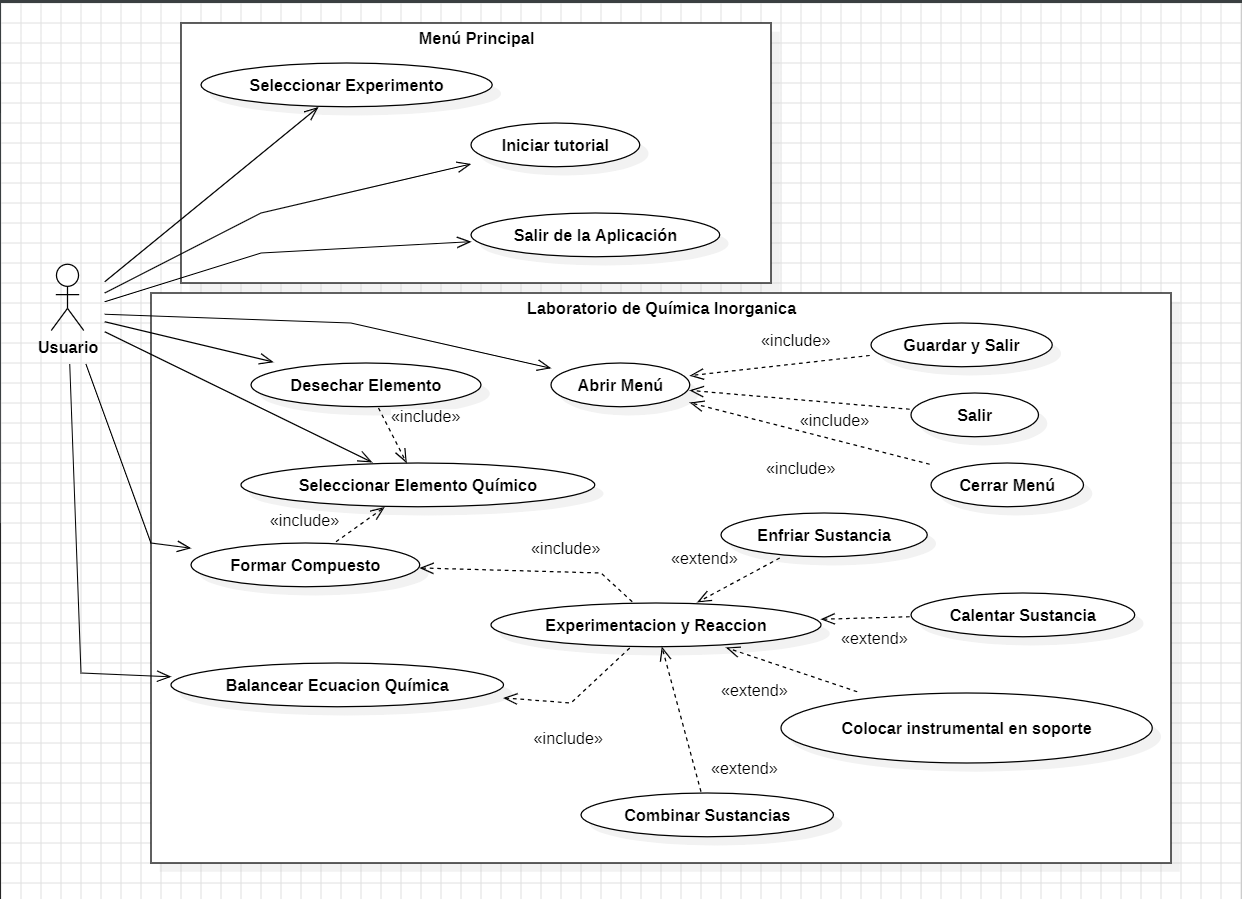
\includegraphics[width=1\textwidth, height=12cm]{img/chapter03/Casos de Uso.png}
    \caption{Diagrama de casos de uso para el sistema}\label{fig:Casos de Uso}
\end{figure}
\newpage
\begin{longtable}{>{\raggedright\arraybackslash}m{.25\textwidth} >{\raggedright\arraybackslash}m{.65\textwidth}}
    \toprule\toprule
    \textbf{Caso de Uso} & Seleccionar Experimento \\
    \midrule\midrule
    \endfirsthead

    \toprule\toprule
    \textbf{Caso de Uso} & Seleccionar Experimento \\
    \midrule\midrule
    \endhead

    \midrule
    \multicolumn{2}{r}{\textit{Continúa en la siguiente página}} \\
    \midrule
    \endfoot

    \endlastfoot

    \textbf{Descripción corta} & El usuario elige un experimento de química para realizar en el simulador. \\
    \midrule
    \textbf{Precondición} & El usuario se encuentra en el menú principal del simulador. \\
    \midrule
    \textbf{Postcondición} & El sistema carga el entorno y los materiales del experimento seleccionado, y presenta al usuario las instrucciones iniciales. \\
    \midrule
    \textbf{Situaciones de error} & \textbf{Selección Inválida:} El usuario intenta seleccionar un experimento que no existe o no está disponible.  \\
    \midrule
    \textbf{Actores} & Usuario \\
    \midrule
    \textbf{Disparadores} & El usuario interactúa con la interfaz del menú principal y selecciona un experimento de la lista. \\
    \midrule
    \textbf{Proceso estándar} &
    \begin{enumerate}
        \item El sistema muestra una lista de experimentos disponibles en el menú principal. 
        \item El usuario utiliza el hand tracking para seleccionar un experimento de la lista. 
        \item El sistema verifica la validez de la selección. 
        \item El sistema carga el entorno virtual del laboratorio, incluyendo los materiales y equipos necesarios para el experimento. 
        \item El sistema presenta al usuario las instrucciones iniciales del experimento. 
    \end{enumerate} \\
    \midrule
    \textbf{Procesos alternativos} & \textbf{3A. Selección Inválida: }
    \begin{enumerate}
        \item El sistema detecta que la selección del usuario no es válida.
        \item El sistema muestra un mensaje de error indicando que el experimento no existe o no está disponible.
        \item El sistema regresa al menú principal.
    \end{enumerate}\\
    \midrule
    \caption{Descripción del caso de uso Seleccionar Experimento}
    \label{tab:Caso_de_uso_Seleccionar_Experimento}
\end{longtable}

\begin{longtable}{>{\raggedright\arraybackslash}m{.25\textwidth} >{\raggedright\arraybackslash}m{.65\textwidth}}
    \toprule\toprule
    \textbf{Caso de Uso} & Iniciar Tutorial \\
    \midrule\midrule
    \endfirsthead

    \toprule\toprule
    \textbf{Caso de Uso} & Iniciar Tutorial \\
    \midrule\midrule
    \endhead

    \midrule
    \multicolumn{2}{r}{\textit{Continúa en la siguiente página}} \\
    \midrule
    \endfoot

    \endlastfoot

    \textbf{Descripción corta} &El usuario accede a un tutorial interactivo para aprender a utilizar las funciones básicas del simulador. \\
    \midrule
    \textbf{Precondición} & El usuario se encuentra en el menú principal del simulador. \\
    \midrule
    \textbf{Postcondición} & El usuario ha completado el tutorial y está familiarizado con las interacciones básicas del simulador. \\
    \midrule
    \textbf{Situaciones de error} & No aplica.  \\
    \midrule
    \textbf{Actores} & Usuario \\
    \midrule
    \textbf{Disparadores} & El usuario selecciona la opción Iniciar Tutorial en el menú principal.\\
    \midrule
    \textbf{Proceso estándar} &
    \begin{enumerate}
        \item El sistema presenta una serie de instrucciones y demostraciones interactivas que guían al usuario a través de las funciones básicas del simulador, como la selección de elementos de la tabla periódica, la manipulación de objetos y la realización de mediciones. 
        \item El usuario sigue las instrucciones y completa las tareas interactivas utilizando el hand tracking. 
        \item El sistema proporciona retroalimentación visual y auditiva al usuario sobre su desempeño en cada tarea. 
        \item Una vez completadas todas las tareas del tutorial, el sistema regresa al menú principal.  
    \end{enumerate} \\
    \midrule
    \textbf{Procesos alternativos} & No aplica.\\
    \midrule
    \caption{Descripción del caso de uso Iniciar Tutorial}
    \label{tab:Caso_de_uso_Iniciar_Tutorial}
\end{longtable}

\begin{longtable}{>{\raggedright\arraybackslash}m{.25\textwidth} >{\raggedright\arraybackslash}m{.65\textwidth}}
    \toprule\toprule
    \textbf{Caso de Uso} &  Balancear Ecuación Química \\
    \midrule\midrule
    \endfirsthead

    \toprule\toprule
    \textbf{Caso de Uso} &  Balancear Ecuación Química \\
    \midrule\midrule
    \endhead

    \midrule
    \multicolumn{2}{r}{\textit{Continúa en la siguiente página}} \\
    \midrule
    \endfoot

    \endlastfoot

    \textbf{Descripción corta} & El usuario balancea una ecuación química proporcionada por el sistema. \\
    \midrule
    \textbf{Precondición} & El sistema ha presentado al usuario una ecuación química desbalanceada como parte de un experimento. \\
    \midrule
    \textbf{Postcondición} & El usuario ha balanceado correctamente la ecuación química, y el sistema lo verifica y permite avanzar al siguiente paso del experimento.  \\
    \midrule
    \textbf{Situaciones de error} & \textbf{Balanceo Incorrecto:} El usuario intenta confirmar un balanceo incorrecto de la ecuación.   \\
    \midrule
    \textbf{Actores} & Usuario \\
    \midrule
    \textbf{Disparadores} & El sistema presenta una ecuación química desbalanceada y solicita al usuario que la balancee.\\
    \midrule
    \textbf{Proceso estándar} &
    \begin{enumerate}
        \item El sistema muestra la ecuación química desbalanceada en la interfaz de usuario. 
        \item El usuario utiliza el hand tracking para interactuar con los coeficientes de la ecuación, incrementándolos o decrementándolos según sea necesario. 
        \item El usuario confirma que ha terminado de balancear la ecuación. 
        \item El sistema verifica si la ecuación está balanceada correctamente. 
        \item Si la ecuación está balanceada, el sistema permite al usuario avanzar al siguiente paso del experimento.  
    \end{enumerate} \\
    \midrule
    \textbf{Procesos alternativos} & 4A. \textbf{Balanceo Incorrecto: }
    \begin{itemize}
        \item El sistema detecta que la ecuación no está balanceada correctamente. 
        \item El sistema muestra un mensaje de error indicando que el balanceo es incorrecto. 
        \item El sistema permite al usuario seguir intentando balancear la ecuación. 
    \end{itemize}\\
    \midrule
    \caption{Descripción del caso de uso  Balancear Ecuación Química}
    \label{tab:Caso_de_uso_ Balancear_Ecuación_Química}
\end{longtable}

\begin{longtable}{>{\raggedright\arraybackslash}m{.25\textwidth} >{\raggedright\arraybackslash}m{.65\textwidth}}
    \toprule\toprule
    \textbf{Caso de Uso} &  Seleccionar Elemento Químico \\
    \midrule\midrule
    \endfirsthead

    \toprule\toprule
    \textbf{Caso de Uso} &  Seleccionar Elemento Químico \\
    \midrule\midrule
    \endhead

    \midrule
    \multicolumn{2}{r}{\textit{Continúa en la siguiente página}} \\
    \midrule
    \endfoot

    \endlastfoot

    \textbf{Descripción corta} &  El usuario selecciona un elemento químico de la tabla periódica interactiva.  \\
    \midrule
    \textbf{Precondición} & La tabla periódica interactiva está visible en la interfaz del usuario.  \\
    \midrule
    \textbf{Postcondición} & 
    \begin{itemize}
        \item El elemento seleccionado se resalta visualmente en la tabla periódica. 
        \item Se muestra información detallada sobre el elemento seleccionado en una interfaz separada. 
        \item Se genera un modelo 3D del elemento seleccionado en el área de trabajo. 
    \end{itemize}\\
    \midrule
    \textbf{Situaciones de error} & No aplica. \\
    \midrule
    \textbf{Actores} & Usuario \\
    \midrule
    \textbf{Disparadores} & El usuario toca un elemento químico en la tabla periódica interactiva utilizando el hand tracking.\\
    \midrule
    \textbf{Proceso estándar} &
    \begin{enumerate}
        \item El usuario toca un elemento químico en la tabla periódica interactiva. 
        \item El sistema detecta la selección y resalta visualmente el elemento. 
        \item El sistema recupera información detallada sobre el elemento seleccionado (nombre, símbolo, número atómico, masa atómica, etc.) y la muestra en una interfaz de usuario separada. 
        \item El sistema genera un modelo 3D del elemento seleccionado y lo coloca en el área de trabajo.  
    \end{enumerate} \\
    \midrule
    \textbf{Procesos alternativos} & No aplica. \\
    \midrule
    \caption{Descripción del caso de uso  Seleccionar Elemento Químico}
    \label{tab:Caso_de_uso_ Balancear_Seleccionar_Elemento_Químico}
\end{longtable}

\begin{longtable}{>{\raggedright\arraybackslash}m{.25\textwidth} >{\raggedright\arraybackslash}m{.65\textwidth}}
    \toprule\toprule
    \textbf{Caso de Uso} &  Crear Compuesto \\
    \midrule\midrule
    \endfirsthead

    \toprule\toprule
    \textbf{Caso de Uso} &  Crear Compuesto \\
    \midrule\midrule
    \endhead

    \midrule
    \multicolumn{2}{r}{\textit{Continúa en la siguiente página}} \\
    \midrule
    \endfoot

    \endlastfoot

    \textbf{Descripción corta} &  El usuario crea un compuesto químico combinando elementos seleccionados de la tabla periódica. \\
    \midrule
    \textbf{Precondición} & 
    \begin{itemize}
        \item El usuario ha seleccionado los elementos químicos necesarios para formar el compuesto. 
        \item Los elementos seleccionados están presentes en el área de trabajo. 
    \end{itemize}\\
    \midrule
    \textbf{Postcondición} & 
    \begin{itemize}
        \item El sistema genera un modelo 3D del compuesto formado. 
        \item El modelo 3D del compuesto se coloca en el área de trabajo. 
        \item Los modelos 3D de los elementos utilizados se eliminan del área de trabajo. 
    \end{itemize}\\
    \midrule
    \textbf{Situaciones de error} & 
    \begin{itemize}
        \item \textbf{Combinación Inválida: }El usuario intenta combinar elementos que no forman un compuesto válido. 
        \item \textbf{Elementos Insuficientes: }El usuario no ha seleccionado todos los elementos necesarios para formar el compuesto. 
    \end{itemize}\\
    \midrule
    \textbf{Actores} & Usuario \\
    \midrule
    \textbf{Disparadores} & El usuario toca un elemento químico en la tabla periódica interactiva utilizando el hand tracking.\\
    \midrule
    \textbf{Proceso estándar} &
    \begin{enumerate}
        \item El usuario indica al sistema que desea crear un compuesto. 
        \item El sistema verifica si la combinación de elementos es válida y si todos los elementos necesarios están presentes. 
        \item Si la combinación es válida, el sistema genera un modelo 3D del compuesto y lo coloca en el área de trabajo. 
        \item El sistema elimina los modelos 3D de los elementos utilizados.  
    \end{enumerate} \\
    \midrule
    \textbf{Procesos alternativos} & 
    \begin{enumerate}[{2}A. ]
        \item \textbf{Combinación Inválida: }
        \begin{itemize}
            \item El sistema detecta que la combinación de elementos no es válida. 
            \item El sistema muestra un mensaje de error indicando que la combinación no es posible. 
            \item El sistema permite al usuario seleccionar otros elementos o cancelar la creación del compuesto.
        \end{itemize}
        \item \textbf{Elementos Insuficientes: }
        \begin{itemize}
            \item El sistema detecta que faltan elementos para formar el compuesto. 
            \item El sistema muestra un mensaje de error indicando los elementos faltantes. 
            \item El sistema permite al usuario seleccionar los elementos faltantes o cancelar la creación del compuesto. 
        \end{itemize}      
    \end{enumerate}\\
    \midrule
    \caption{Descripción del caso de uso Crear Compuesto}
    \label{tab:Caso_de_uso_ Balancear_Crear_Compuesto}
\end{longtable}

\begin{longtable}{>{\raggedright\arraybackslash}m{.25\textwidth} >{\raggedright\arraybackslash}m{.65\textwidth}}
    \toprule\toprule
    \textbf{Caso de Uso} &   Calentar Compuesto \\
    \midrule\midrule
    \endfirsthead

    \toprule\toprule
    \textbf{Caso de Uso} &   Calentar Compuesto \\
    \midrule\midrule
    \endhead

    \midrule
    \multicolumn{2}{r}{\textit{Continúa en la siguiente página}} \\
    \midrule
    \endfoot

    \endlastfoot

    \textbf{Descripción corta} &  El usuario calienta un compuesto utilizando un mechero Bunsen. \\
    \midrule
    \textbf{Precondición} & 
    \begin{itemize}
        \item El mechero Bunsen está disponible y encendido. 
        \item El usuario se encuentra en una etapa del experimento que requiere calentar un compuesto. 
    \end{itemize}\\
    \midrule
    \textbf{Postcondición} &  El compuesto válido se calienta y se muestran los cambios visuales y auditivos correspondientes.\\
    \midrule
    \textbf{Situaciones de error} & El usuario intenta calentar una sustancia o compuesto no válido.\\
    \midrule
    \textbf{Actores} & Usuario \\
    \midrule
    \textbf{Disparadores} & El usuario acerca el compuesto al mechero Bunsen.\\
    \midrule
    \textbf{Proceso estándar} &
    \begin{enumerate}
        \item El usuario selecciona el mechero Bunsen y lo acerca a la sustancia o compuesto (Controlador). 
        \item El sistema verifica si la sustancia o compuesto es válido para calentar (Modelo). 
        \item Si es válido, el sistema detecta la proximidad y activa el calentamiento (Modelo). 
        \item El sistema simula el efecto del calor en el compuesto, mostrando cambios visuales (burbujas, cambio de color) y auditivos (sonido de ebullición) (Vista). 
    \end{enumerate} \\
    \midrule
    \textbf{Procesos alternativos} & 
    \begin{enumerate}[{2}A. ]
        \item \textbf{Sustancia o Compuesto No Válido:} Si la sustancia o compuesto no es válido, el sistema muestra un mensaje de error.     
    \end{enumerate}\\
    \midrule
    \caption{Descripción del caso de uso Calentar Compuesto}
    \label{tab:Caso_de_uso_ Balancear_Calentar_Compuesto}
\end{longtable}

\begin{longtable}{>{\raggedright\arraybackslash}m{.25\textwidth} >{\raggedright\arraybackslash}m{.65\textwidth}}
    \toprule\toprule
    \textbf{Caso de Uso} &   Enfriar Compuesto \\
    \midrule\midrule
    \endfirsthead

    \toprule\toprule
    \textbf{Caso de Uso} &   Enfriar Compuesto \\
    \midrule\midrule
    \endhead


    \endfoot

    \endlastfoot
    \textbf{Descripción corta} &  El usuario sumerge un vaso de precipitados que contiene una solución en un baño de agua para disminuir su temperatura y observar los cambios resultantes. \\
    \midrule
    \textbf{Precondición} & 
    \begin{itemize}
        \item El vaso de precipitados con la solución a enfriar está presente en el área de trabajo. 
        \item El baño de agua está disponible. 
        \item El usuario se encuentra en una etapa del experimento que requiere enfriar la solución 
    \end{itemize}\\
    \midrule
    \textbf{Postcondición} &  El compuesto válido se enfría y se muestran los cambios visuales correspondientes.\\
    \midrule
    \textbf{Situaciones de error} & El usuario intenta enfriar una sustancia o compuesto no válido.\\
    \midrule
    \textbf{Actores} & Usuario \\
    \midrule
    \textbf{Disparadores} & El usuario acerca el recipiente al baño de agua.\\
    \midrule
    \textbf{Proceso estándar} &
    \begin{enumerate}
        \item El usuario selecciona el recipiente que contiene el compuesto y lo sumerge en el baño de hielo (Controlador). 
        \item El sistema verifica si la sustancia o compuesto es válido para enfriar (Modelo). 
        \item Si es válido, el sistema detecta la inmersión y activa el enfriamiento (Modelo). 
        \item El sistema simula el efecto del enfriamiento en el compuesto (Vista).  
    \end{enumerate} \\
    \midrule
    \textbf{Procesos alternativos} & 
    \begin{enumerate}[{2}A. ]
        \item \textbf{Sustancia o Compuesto No Válido:} Si la sustancia o compuesto no es válido, el sistema muestra un mensaje de error. 
    \end{enumerate}\\
    \midrule
    \caption{Descripción del caso de uso Enfriar Compuesto}
    \label{tab:Caso_de_uso_ Balancear_Enfriar_Compuesto}
\end{longtable}

\begin{longtable}{>{\raggedright\arraybackslash}m{.25\textwidth} >{\raggedright\arraybackslash}m{.65\textwidth}}
    \toprule\toprule
    \textbf{Caso de Uso} &   Combinar Sustancias \\
    \midrule\midrule
    \endfirsthead

    \toprule\toprule
    \textbf{Caso de Uso} &   Combinar Sustancias \\
    \midrule\midrule
    \endhead

    \midrule
    \multicolumn{2}{r}{\textit{Continúa en la siguiente página}} \\
    \midrule
    \endfoot

    \endlastfoot

    \textbf{Descripción corta} & El usuario combina dos o más sustancias en un nuevo recipiente para iniciar una reacción química.\\
    \midrule
    \textbf{Precondición} & Las sustancias a combinar están disponibles en el área de trabajo.\\
    \midrule
    \textbf{Postcondición} & Las sustancias válidas se combinan en un nuevo recipiente y se produce la reacción química, mostrando los cambios visuales y auditivos correspondientes.\\
    \midrule
    \textbf{Situaciones de error} & El usuario intenta combinar sustancias no válidas.\\
    \midrule
    \textbf{Actores} & Usuario \\
    \midrule
    \textbf{Disparadores} & El usuario arrastra las sustancias seleccionadas a un nuevo recipiente.\\
    \midrule
    \textbf{Proceso estándar} &
    \begin{enumerate}
        \item El usuario selecciona las sustancias que desea combinar y las arrastra al recipiente (Controlador). 
        \item El sistema verifica la validez de las sustancias para ser combinadas (Modelo). 
        \item Si son compatibles, el sistema simula la combinación y la reacción química, mostrando cambios visuales y auditivos (Vista).  
    \end{enumerate} \\
    \midrule
    \textbf{Procesos alternativos} & 
    \begin{enumerate}[{2}A. ]
        \item \textbf{Combinación Inválida:} Si las sustancias no son compatibles, el sistema muestra un mensaje de error.
    \end{enumerate}\\
    \midrule
    \caption{Descripción del caso de uso Combinar Sustancias}
    \label{tab:Caso_de_uso_ Balancear_Combinar_Sustancias}
\end{longtable}

\begin{longtable}{>{\raggedright\arraybackslash}m{.25\textwidth} >{\raggedright\arraybackslash}m{.65\textwidth}}
    \toprule\toprule
    \textbf{Caso de Uso} & Desechar elemento \\
    \midrule\midrule
    \endfirsthead

    \toprule\toprule
    \textbf{Caso de Uso} & Desechar elemento \\
    \midrule\midrule
    \endhead

    \midrule
    \multicolumn{2}{r}{\textit{Continúa en la siguiente página}} \\
    \midrule
    \endfoot

    \endlastfoot

    \textbf{Descripción corta} & El usuario elimina un elemento del área de trabajo.\\
    \midrule
    \textbf{Precondición} & 
    \begin{itemize}
        \item \textbf{Existencia del Elemento:} El elemento a desechar debe estar presente y visible en el área de trabajo.
        \item \textbf{Área de Desecho Habilitada:} El área de desecho debe estar habilitada y accesible para el usuario.
    \end{itemize}\\
    \midrule
    \textbf{Postcondición} & El elemento o compuesto se elimina del área de trabajo.\\
    \midrule
    \textbf{Situaciones de error} & El usuario intenta desechar un elemento que el sistema no permite eliminar en ese momento del experimento.\\
    \midrule
    \textbf{Actores} & Usuario \\
    \midrule
    \textbf{Disparadores} &  El usuario deposita el elemento en el área de desecho.\\
    \midrule
    \textbf{Proceso estándar} &
    \begin{enumerate}
        \item \textbf{Inicio:} El usuario toma el elemento o compuesto a desechar.
        \item \textbf{Movimiento}: El usuario mueve el elemento o compuesto hacia el área de desecho.
        \item \textbf{Soltar:} El usuario suelta el elemento o compuesto dentro de los límites del área de desecho.
        \item \textbf{Validación:} El sistema valida que el elemento o compuesto puede ser desechado en ese momento del experimento.
        \item \textbf{Eliminación:} El sistema elimina el elemento o compuesto del área de trabajo y de cualquier estructura de datos asociada.
    \end{enumerate} \\
    \midrule
    \textbf{Procesos alternativos} & 
    \begin{enumerate}[{4}A. ]
        \item Validación: El sistema detecta que el elemento o compuesto no puede ser desechado en ese momento.
        \item Notificación: El sistema muestra un mensaje de error claro indicando que el elemento o compuesto no puede ser desechado en ese momento.
        \item Cancelación: El elemento o compuesto regresa a su posición original en el área de trabajo.
    \end{enumerate}\\
    \midrule
    \caption{Descripción del caso de uso Desechar elemento}
    \label{tab:Caso_de_uso_ Balancear_Desechar_elemento}
\end{longtable}

\begin{longtable}{>{\raggedright\arraybackslash}m{.25\textwidth} >{\raggedright\arraybackslash}m{.65\textwidth}}
    \toprule\toprule
    \textbf{Caso de Uso} & Experimentación y Reacción \\
    \midrule\midrule
    \endfirsthead

    \toprule\toprule
    \textbf{Caso de Uso} & Experimentación y Reacción \\
    \midrule\midrule
    \endhead

    \midrule
    \multicolumn{2}{r}{\textit{Continúa en la siguiente página}} \\
    \midrule
    \endfoot

    \endlastfoot

    \textbf{Descripción corta} & El usuario interactúa con los compuestos y el instrumental para realizar la experimentación y reacción química, mientras el sistema simula los efectos.\\
    \midrule
    \textbf{Precondición} & 
    \begin{itemize}
        \item \textbf{Compuestos disponibles:} Los compuestos químicos necesarios para el experimento se seleccionaron y están en el área de trabajo virtual.
        \item \textbf{Instrumental disponible: }El instrumental virtual requerido (matraces, pipetas, mecheros, etc.) está presente y accesible en el área de trabajo.
    \end{itemize}\\
    \midrule
    \textbf{Postcondición} & 
    \begin{itemize}
        \item \textbf{Resultados simulados:} El sistema ha simulado los resultados de la reacción o experimento químico realizado por el usuario.
        \item \textbf{Visualización de resultados:} El usuario puede observar los cambios en los compuestos, la formación de nuevos productos, cambios de temperatura, etc., en la interfaz del sistema.
    \end{itemize}\\
    \midrule
    \textbf{Situaciones de error} & 
    \begin{itemize}
        \item \textbf{Compuestos Insuficientes:} El usuario intenta realizar un experimento sin todos los compuestos necesarios.
        \item \textbf{Acciones Inválidas:} Si el usuario intenta realizar una acción no permitida por el diseño del experimento, el sistema lo notificará y detendrá la simulación.
    \end{itemize}\\
    \midrule
    \textbf{Actores} & Usuario \\
    \midrule
    \textbf{Disparadores} &  El usuario comienza a interactuar con los compuestos o el instrumental virtual.\\
    \midrule
    \textbf{Proceso estándar} &
    \begin{enumerate}
        \item \textbf{Inicio:} El usuario toma el elemento o compuesto a desechar.
        \item \textbf{Movimiento}: El usuario mueve el elemento o compuesto hacia el área de desecho.
        \item \textbf{Soltar:} El usuario suelta el elemento o compuesto dentro de los límites del área de desecho.
        \item \textbf{Validación:} El sistema valida que el elemento o compuesto puede ser desechado en ese momento del experimento.
        \item \textbf{Eliminación:} El sistema elimina el elemento o compuesto del área de trabajo y de cualquier estructura de datos asociada.
    \end{enumerate} \\
    \midrule
    \textbf{Procesos alternativos} & 
    \begin{enumerate}[{4}A. ]
        \item Validación: El sistema detecta que el elemento o compuesto no puede ser desechado en ese momento.
        \item Notificación: El sistema muestra un mensaje de error claro indicando que el elemento o compuesto no puede ser desechado en ese momento.
        \item Cancelación: El elemento o compuesto regresa a su posición original en el área de trabajo.
    \end{enumerate}\\
    \midrule
    \caption{Descripción del caso de uso Experimentación y Reacción}
    \label{tab:Caso_de_uso_ Balancear_Experimentación_y_Reacción}
\end{longtable}

\begin{longtable}{>{\raggedright\arraybackslash}m{.25\textwidth} >{\raggedright\arraybackslash}m{.65\textwidth}}
    \toprule\toprule
    \textbf{Caso de Uso} & Main Menu \\
    \midrule\midrule
    \endfirsthead

    \toprule\toprule
    \textbf{Caso de Uso} & Main Menu \\
    \midrule\midrule
    \endhead

    \midrule
    \multicolumn{2}{r}{\textit{Continúa en la siguiente página}} \\
    \midrule
    \endfoot

    \endlastfoot

    \textbf{Descripción corta} &El usuario sale del experimento actual y regresa al menú de bienvenida. \\
    \midrule
    \textbf{Precondición} & El usuario se encuentra en el Menú del escenario de un experimento.\\
    \midrule
    \textbf{Postcondición} &  El experimento actual se cierra y el usuario regresa al menú de bienvenida. \\
    \midrule
    \textbf{Situaciones de error} & Ninguna\\
    \midrule
    \textbf{Actores} & Usuario \\
    \midrule
    \textbf{Disparadores} & El usuario selecciona la opción "Main Menu" en el menú.\\
    \midrule
    \textbf{Proceso estándar} &
    \begin{enumerate}
        \item El sistema detecta la selección de la opción "Main Menu".
        \item El sistema detiene la simulación del experimento actual.
        \item El sistema regresa al menú de bienvenida.
    \end{enumerate} \\
    \midrule
    \textbf{Procesos alternativos} & Ninguno.\\
    \midrule
    \caption{Descripción del caso de uso Main Menu}
    \label{tab:Caso_de_uso_Main_Menu}
\end{longtable}

\begin{longtable}{>{\raggedright\arraybackslash}m{.25\textwidth} >{\raggedright\arraybackslash}m{.65\textwidth}}
    \toprule\toprule
    \textbf{Caso de Uso} & Colocar instrumental en soporte \\
    \midrule\midrule
    \endfirsthead

    \toprule\toprule
    \textbf{Caso de Uso} & Colocar instrumental en soporte\\
    \midrule\midrule
    \endhead

    \midrule
    \multicolumn{2}{r}{\textit{Continúa en la siguiente página}} \\
    \midrule
    \endfoot

    \endlastfoot

    \textbf{Descripción corta} &El usuario coloca un instrumento de laboratorio en un soporte designado. \\
    \midrule
    \textbf{Precondición} & El usuario está sosteniendo un instrumento de laboratorio con la mano y hay un soporte disponible.\\
    \midrule
    \textbf{Postcondición} & El instrumento de laboratorio se coloca en el soporte y se libera de la mano del usuario. \\
    \midrule
    \textbf{Situaciones de error} & No hay un soporte disponible o el usuario no está sosteniendo un instrumento compatible con el soporte. \\
    \midrule
    \textbf{Actores} & Usuario \\
    \midrule
    \textbf{Disparadores} & El usuario acerca el instrumento al soporte y realiza el gesto de "soltar". \\
    \midrule
    \textbf{Proceso estándar} &
    \begin{enumerate}
        \item El sistema detecta que el usuario está acercando un instrumento a un soporte.
        \item El sistema verifica si el soporte está disponible y si el instrumento es compatible.
        \item Si el soporte está disponible y el instrumento es compatible, el sistema coloca el instrumento en el soporte y lo libera de la mano del usuario.
    \end{enumerate} \\
    \midrule
    \textbf{Procesos alternativos} & 3A. Si el soporte no está disponible o el instrumento no es compatible, el sistema muestra un mensaje de error al usuario..\\
    \midrule
    \caption{Descripción del caso de uso Colocar instrumental en soporte}
    \label{tab:Caso_de_uso_Colocar_instrumental_en_soporte}
\end{longtable}
\newpage
\subsection{Diagrama de Clases}
\begin{figure}[thbp]
    \centering
    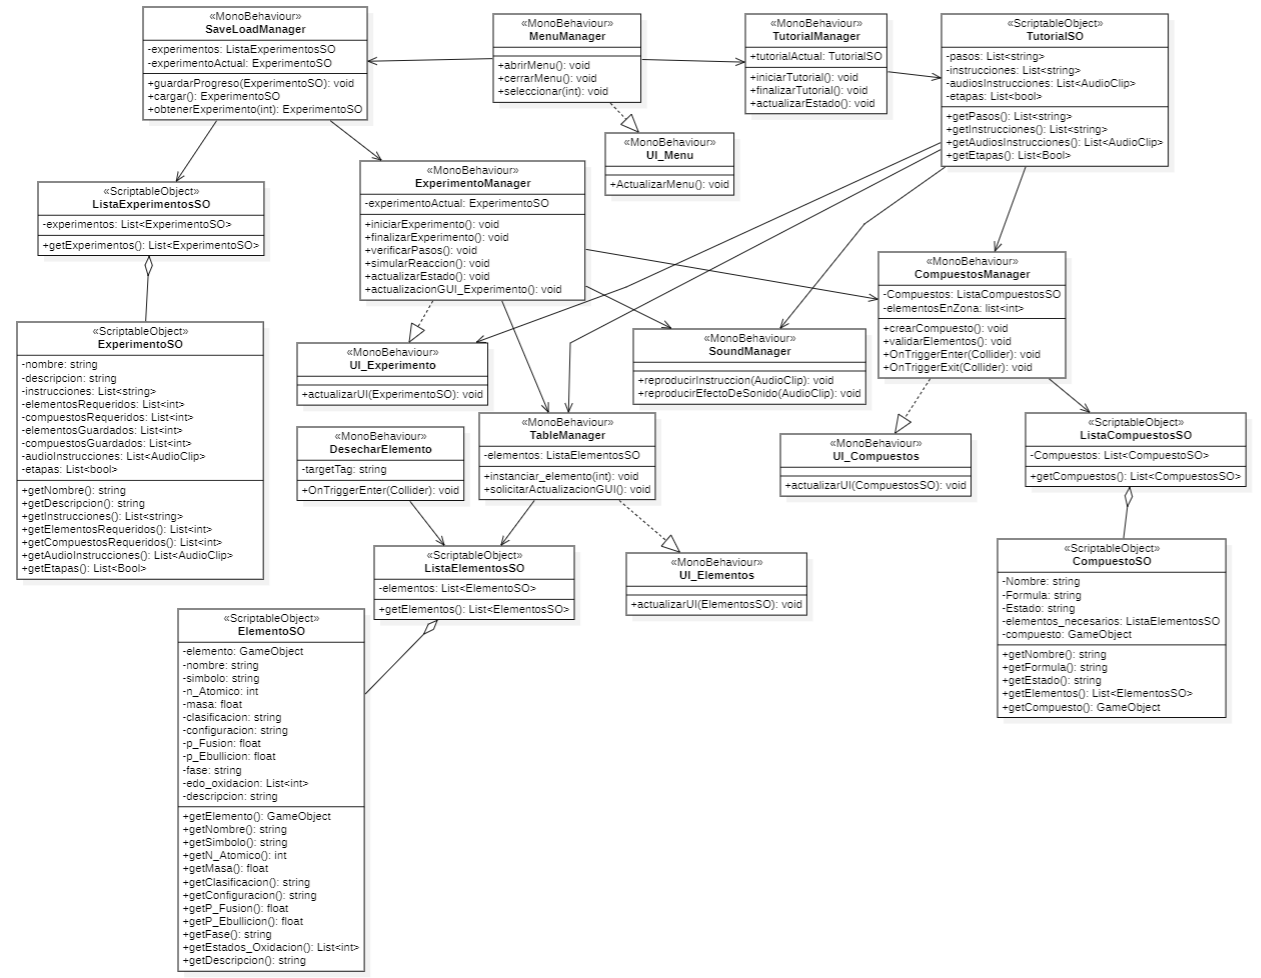
\includegraphics[width=0.9\textwidth, height = 15cm]{img/chapter03/Diagrama de Clases.png}
    \caption{Diagrama de Clases}
    \label{fig:Diagrama_de_Clases}
\end{figure}
    \chapter{Desarrollo}\label{ch:Desarrollo}
\section{Estructura del Simulador}
En el desarrollo del prototipo de simulador de laboratorio de Química Inorgánica en Realidad Virtual, la organización del proyecto en Unity desempeña un papel crucial para mantener un entorno de desarrollo estructurado, escalable y mantenible. Al crear un proyecto nuevo en Unity, se genera una carpeta principal llamada Assets, que contiene todos los recursos necesarios para el correcto funcionamiento del simulador.

\begin{figure}[thbp]
    \centering
    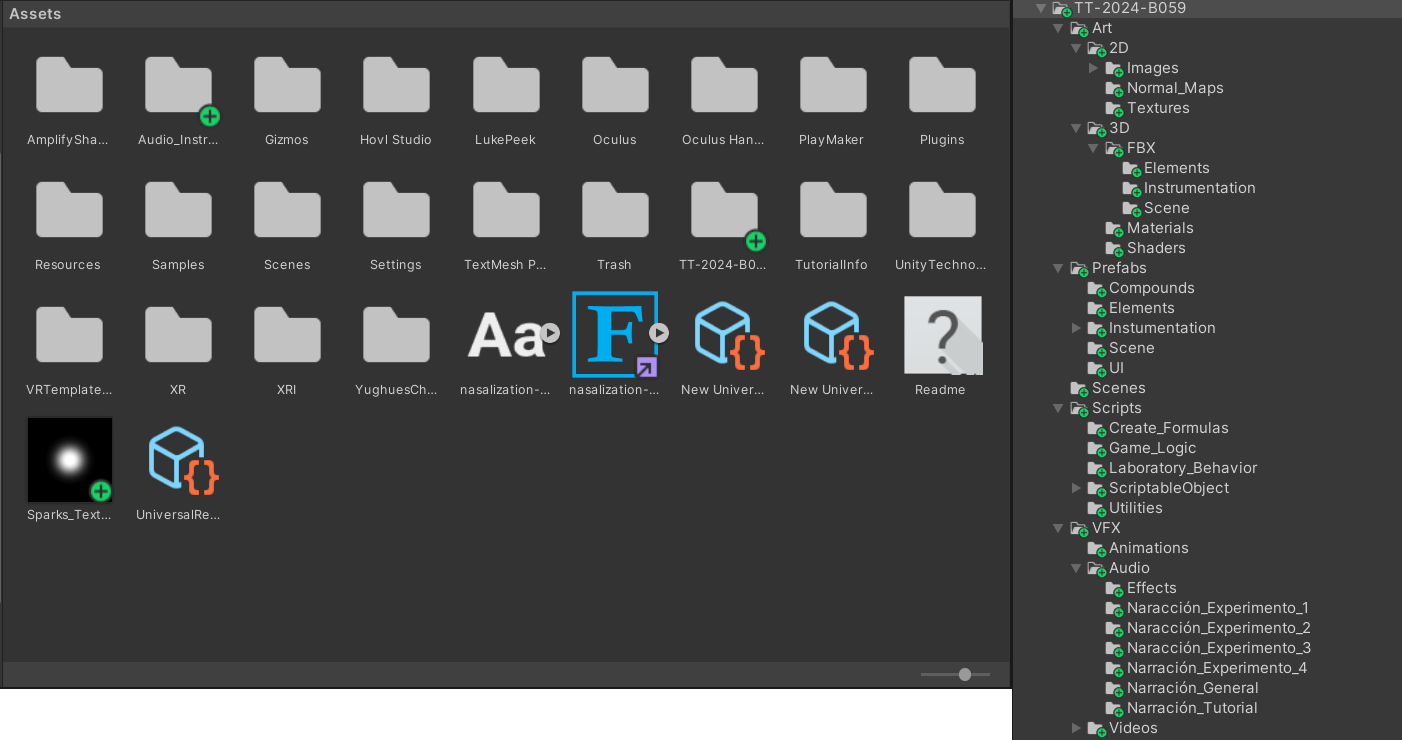
\includegraphics[width=0.8\textwidth, height = 7cm]{img/chapter04/Estructura.png}
    \caption{Assets del Simulador}
    \label{fig:Assets_del_Simulador}
\end{figure}

Esta carpeta se subdivide en varias carpetas específicas según su propósito, como se detalla a continuación:

\begin{enumerate} [I. ]
    \item \textit{\textbf{Art}}:
    
    Esta carpeta contiene los recursos gráficos utilizados en el simulador, divididos en dos subcarpetas principales:
    \begin{itemize}
        \item \textbf{2D}: Incluye imágenes, mapas normales y texturas utilizadas para enriquecer los elementos visuales del entorno.
        \newpage
        \item \textbf{3D}: Contiene modelos tridimensionales organizados en:
        \begin{itemize}
            \item FBX: Modelos de elementos, instrumental y escenas del laboratorio.
            \item Materials: Materiales aplicados a los modelos para simular texturas y propiedades físicas.
            \item Shaders\_Graphs: Gráficos de sombreado personalizados que mejoran el realismo del entorno virtual.
        \end{itemize}
    \end{itemize}

    \item \textit{\textbf{Prefabs}}:
    
    Los prefabs son objetos prediseñados con configuraciones preestablecidas, lo que permite reutilizarlos en múltiples escenas. Están organizados en:
    \begin{itemize}
        \item \textbf{Compounds}: Compuestos químicos modelados y configurados con comportamientos específicos.
        \item \textbf{Elements}: Elementos químicos individuales listos para ser utilizados en las simulaciones.
        \item \textbf{Instrumentation}: Herramientas e instrumentos del laboratorio como matraces, tubos de ensayo y mecheros.
        \item \textbf{Scene}: Componentes específicos para gestionar aspectos visuales y funcionales de las escenas.
        \item \textbf{UI}: Elementos de interfaz de usuario diseñados para facilitar la interacción.
    \end{itemize}

    \item \textit{\textbf{Scenes:}}
    
    Esta carpeta contiene todas las escenas creadas para el simulador
    \begin{itemize}
        \item \textbf{Experimentos}: Cada experimento tiene su propia escena, diseñada específicamente para simular procedimientos y reacciones químicas.
        \item \textbf{Tutorial}: Provee instrucciones guiadas para familiarizar al usuario con el simulador y las actividades.
        \item \textbf{Hub}: Actúa como un menú principal donde el usuario puede navegar hacia diferentes experimentos o tutoriales.
    \end{itemize}

    \item \textit{\textbf{Scripts}}:
    
    Contiene todos los scripts de código fuente en lenguaje C\#, organizados según su funcionalidad en las siguientes subcarpetas:
    \begin{itemize}
        \item \textbf{Create\_Formulas}: Scripts para crear y gestionar las fórmulas químicas utilizadas en el simulador.
        \item \textbf{Game\_Logic}: Lógica general del simulador, como eventos y reglas específicas.
        \item \textbf{Laboratory\_Behavior}: Comportamientos de los elementos interactivos del laboratorio.
        \item \textbf{ScriptableObject}: Configuraciones y datos reutilizables en formato ScriptableObject.
        \item \textbf{Utilities}: Scripts auxiliares que apoyan funcionalidades generales del simulador.
    \end{itemize}
    Los scripts se desarrollan siguiendo principios de programación orientada a objetos, aplicando el uso de máquinas de estado para la gestión de escenas y experimentos.

    \item \textit{\textbf{VFX}}:
    
    Esta carpeta contiene los efectos visuales y auditivos que mejoran la experiencia inmersiva del usuario:
    \begin{itemize}
        \item \textbf{Animations}: Animaciones aplicadas a modelos y elementos interactivos.
        \item \textbf{Audio}: Archivos de sonido organizados en:
        \begin{itemize}
            \item Effects: Efectos de sonido específicos.
            \item Narraciones: Audio dividido en narraciones para tutoriales y experimentos.
        \end{itemize}
        \item \textbf{Videos}: Clips de video utilizados para complementar la experiencia educativa.
    \end{itemize}    
\end{enumerate}

\section{Ambiente Virtual} \label{sec:Ambiente_Virtual}

El ambiente virtual desarrollado para el simulador proporciona un espacio interactivo e inmersivo donde los usuarios pueden realizar diversos experimentos de química inorgánica. Este entorno simula un laboratorio moderno e incluye los elementos necesarios para recrear prácticas científicas de manera eficiente y educativa.
\subsection{Diseño del entorno 3D}
El laboratorio consta de los siguientes elementos principales:
\begin{itemize}
    \item \textbf{Mesa de trabajo}: Área central donde se llevan a cabo los experimentos. Diseñada para proporcionar un espacio virtual amplio y funcional que facilita la manipulación de los objetos.
    \item \textbf{Modelos atómicos de los elementos}: Representaciones tridimensionales de los átomos, diseñadas para ilustrar sus estructuras y propiedades.
    \begin{figure}[thbp]
        \centering
        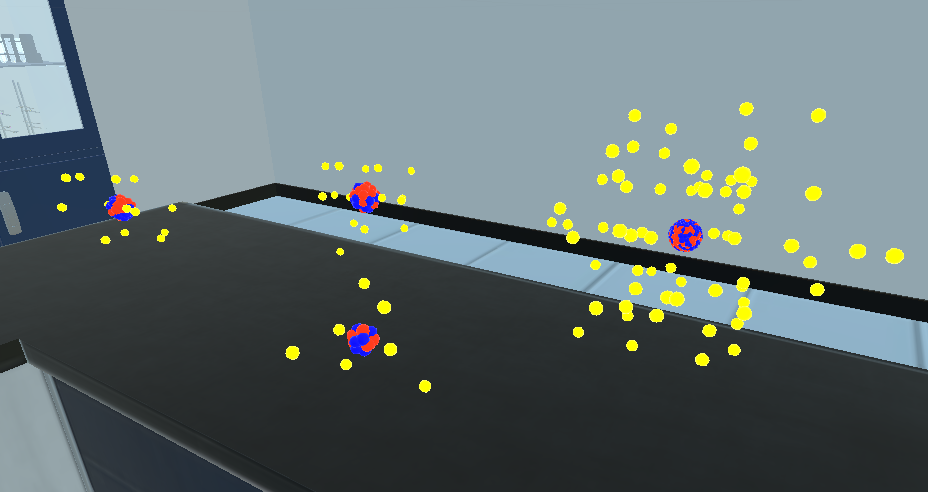
\includegraphics[width=0.6\textwidth, height = 6cm]{img/chapter04/Elementos.png}
        \caption{Modelos de Elementos Químicos}
        \label{fig:Elementos_Químicos}
    \end{figure}
    \newpage
    \item \textbf{Tabla periódica interactiva}: Permite al usuario explorar los elementos químicos de forma dinámica. Al seleccionar un elemento, se despliega información relevante y un modelo atómico tridimensional.
    \begin{figure}[thbp]
        \centering
        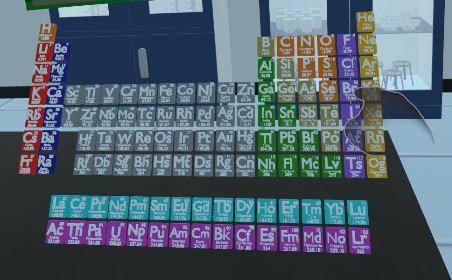
\includegraphics[width=0.6\textwidth, height = 5cm]{img/chapter05/Tabla_Periodica.png}
        \caption{Tabla Periódica}
        \label{fig:Tabla_Periódica}
    \end{figure}

    \item \textbf{Instrumental necesario}: Incluye matraces, tubos de ensayo, mecheros y demás herramientas esenciales, modeladas en detalle para reflejar con precisión el equipo utilizado en laboratorios reales.
    \begin{figure}[thbp]
        \centering
        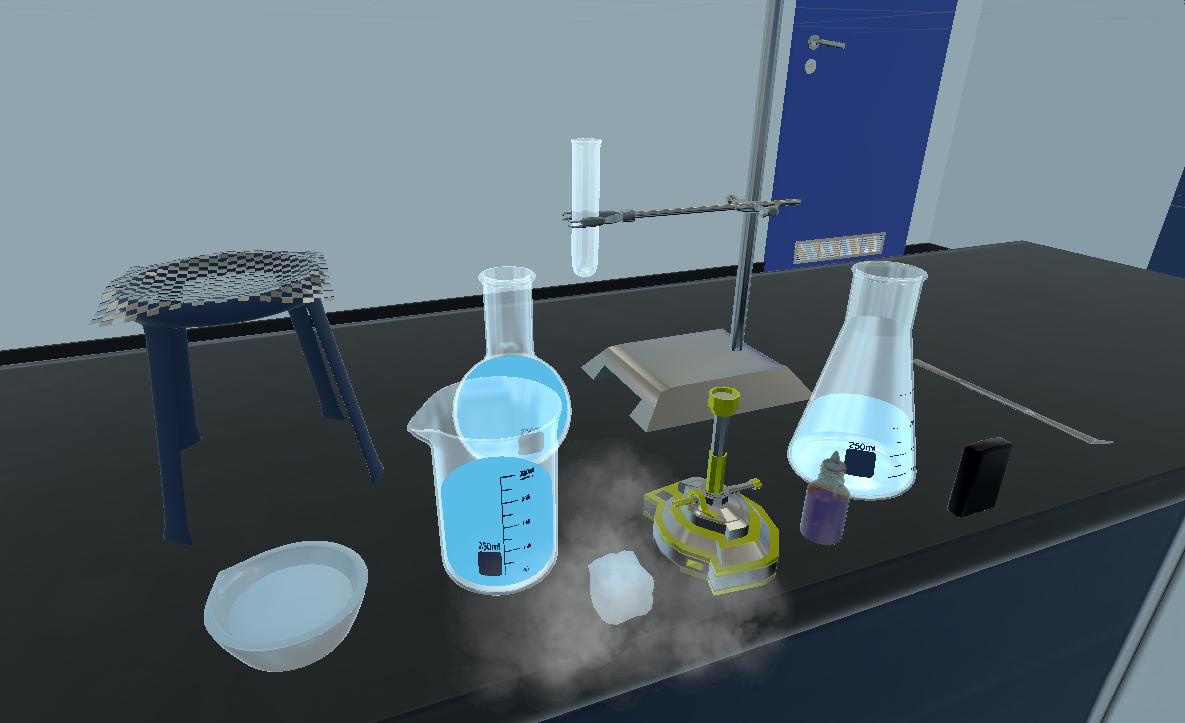
\includegraphics[width=0.6\textwidth, height = 6cm]{img/chapter04/Instrumental.png}
        \caption{Instrumental de Laboratorio}
        \label{fig:Instrumental_De_Laboratorio}
    \end{figure}
    \newpage
    \item \textbf{Modelos de compuestos químicos}: Reproducciones de los compuestos que se generan durante los experimentos, mostrando sus características visuales de manera precisa.
    \begin{figure}[thbp]
        \centering
        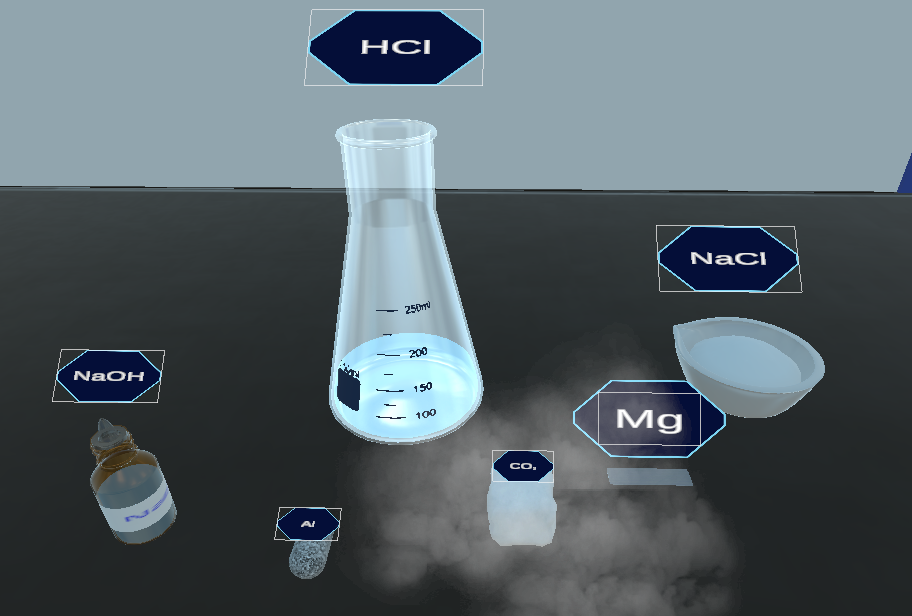
\includegraphics[width=0.6\textwidth, height = 6cm]{img/chapter04/Compuestos.png}
        \caption{Compuestos Químicos}
        \label{fig:Compuestos_Químicos}
    \end{figure}
\end{itemize}

Todo el modelado 3D fue desarrollado utilizando Blender, una herramienta ampliamente reconocida en la industria por su capacidad para crear modelos tridimensionales detallados y eficientes. Las texturas y materiales de estos modelos se trabajaron en GIMP.

\subsection{Efectos Visuales (VFX)}
Para mejorar la inmersión y reforzar la representación de las reacciones químicas y los fenómenos experimentales, se diseñaron una variedad de efectos de partículas. Entre los principales se encuentran:
\begin{itemize}
    \item \textbf{Humo y Vapores}: Representan las liberaciones de gases en ciertas reacciones químicas.
    \item \textbf{Fuego y Chispas}: Simulan encendidos de mecheros y otras reacciones exotérmicas.
    \item \textbf{Niebla}: Utilizada como un efecto visual en reacciones específicas.
\end{itemize}
\begin{figure}[thbp]
    \centering
    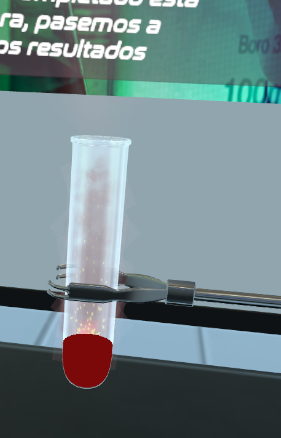
\includegraphics[width=0.6\textwidth, height = 6cm]{img/chapter04/VFX.png}
    \caption{Efectos de Partículas}
    \label{fig:Diversos_Efectos_Visuales}
\end{figure}
Estos efectos se crearon utilizando el Unity Particle System y shaders personalizados para lograr una integración fluida con el entorno.

\subsection{Efectos de Sonido}
El sonido juega un papel fundamental en la inmersión sensorial del simulador. Se incorporaron diversos efectos sonoros para acompañar las interacciones y eventos del laboratorio, incluyendo:
\begin{itemize}
    \item \textbf{Cristales}: Simulan el sonido de recipientes de vidrio al ser manipulados o chocados.
    \item \textbf{Burbujeos y flujo de agua}: Representan procesos químicos y líquidos en movimiento.
    \item \textbf{Fuego y gas}: Emulan encendidos de mecheros y escapes controlados de gases.
\end{itemize}

Los sonidos fueron seleccionados y editados para sincronizarse con precisión en tiempo real mediante el sistema de eventos de Unity. Esto asegura que cada acción del usuario esté acompañada de una respuesta auditiva coherente y realista.
\subsection{Instrucciones guiadas con voz}
Para las instrucciones paso a paso, se utilizó el servicio en línea SpeechGen.io, el cual permitió generar voces claras y dinámicas en varios idiomas. Este sistema se integró para:
\begin{itemize}
    \item Proporcionar guías auditivas que refuercen las instrucciones visuales.
    \item Sincronizar las instrucciones de voz con las acciones y eventos dentro del laboratorio, mejorando la accesibilidad y la experiencia del usuario.
\end{itemize}

\section{Diseño de Interfaz de Usuario}
El diseño de la interfaz de usuario (IU) para el simulador se desarrolló con un enfoque en maximizar la funcionalidad y la accesibilidad dentro del entorno de realidad virtual (RV), adaptándose a las necesidades de un laboratorio químico interactivo. Estas interfaces, aunque densas en información, fueron optimizadas para que los usuarios puedan acceder fácilmente a datos relevantes y operar de manera eficiente en un entorno inmersivo.

\subsection{Hub de selección}
Sirve como el punto de entrada al simulador, diseñado para ofrecer una navegación jerarquía y estructurada:
\begin{itemize}
    \item \textbf{Pantalla inicial}: Contiene dos botones principales: Tutorial y Experimentos.
    \item \textbf{Pantalla de selección de experimentos}: Presenta 4 botones, cada uno correspondiente a un experimento disponible y un quinto botón para regresar al menú principal.
    \item \textbf{Pantalla Tutorial-Experimentos}: Proporciona una descripción general de la selección, con su imagen de referencia y dos opciones de navegación, regresar y confirmar.
\end{itemize}
\begin{figure}[thbp]
    \centering
    \begin{subfigure}[b]{0.4\linewidth}
        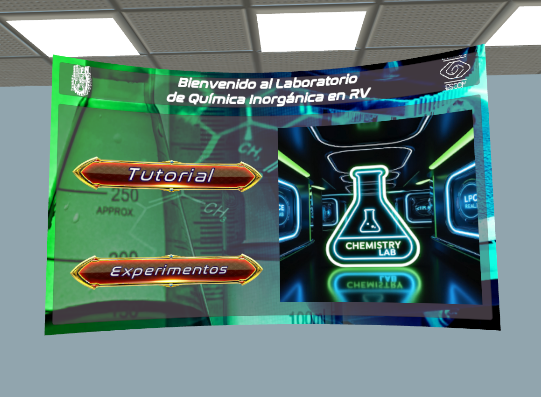
\includegraphics[width=\linewidth, height = 5cm]{img/chapter04/UI_Hub.png}
        \caption{Pantalla Principal Hub}
        \label{fig:Hub_Principal}
    \end{subfigure}
    \begin{subfigure}[b]{0.4\linewidth}
        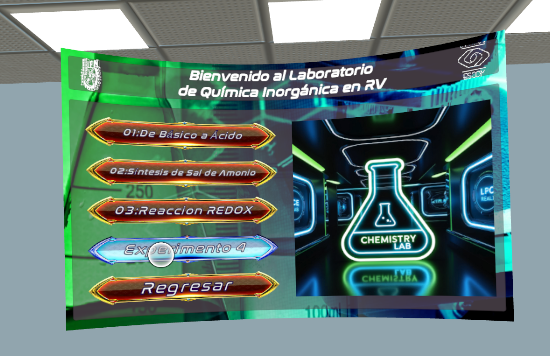
\includegraphics[width=\linewidth, height = 5cm]{img/chapter04/UI_Hub_Experiments.png}
        \caption{Pantalla Selección Experimento}
        \label{fig:Hub_Experimentos}
    \end{subfigure}
    \begin{subfigure}[b]{0.4\linewidth}
        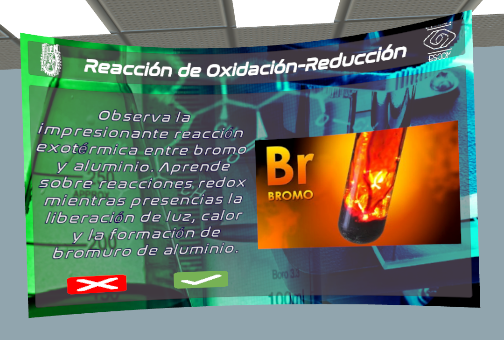
\includegraphics[width=\linewidth, height = 5cm]{img/chapter04/UI_Hub_Experiment.png}
        \caption{Pantalla Información Experimento}
        \label{fig:Hub_Experimento}
    \end{subfigure}
    \caption{IU Hub}
\end{figure}
\newpage
\subsection{Información principal}
Centraliza la información operativa de cada experimento, proporcionando:
\begin{itemize}
    \item Instrucciones detalladas
    \item Soporte visual
    \item Ecuaciones químicas
\end{itemize}
\begin{figure}[thbp]
    \centering
    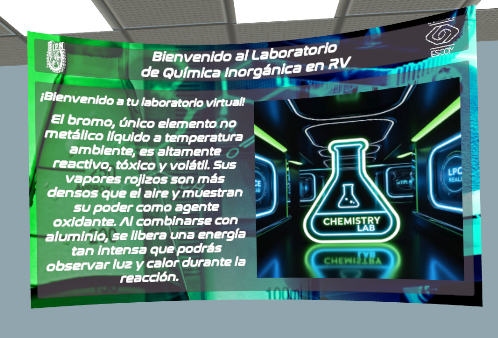
\includegraphics[width=0.6\textwidth, height = 6cm]{img/chapter04/UI_Principal.png}
    \caption{IU Principal}
    \label{fig:Principal_IU}
\end{figure}

\subsection{Elementos}
Se focaliza en proporcionar datos contextuales sobre el último elemento químico seleccionado
\begin{figure}[thbp]
    \centering
    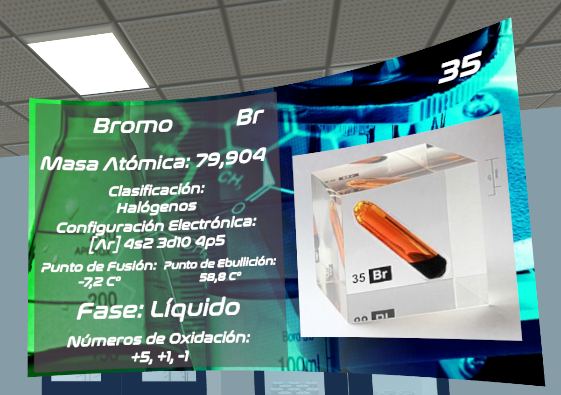
\includegraphics[width=0.6\textwidth, height = 6cm]{img/chapter04/UI_Elements.png}
    \caption{IU Elementos}
    \label{fig:Elementos_IU}
\end{figure}

\subsection{Compuestos}
Presenta información sobre el último compuesto generado.
\begin{figure}[thbp]
    \centering
    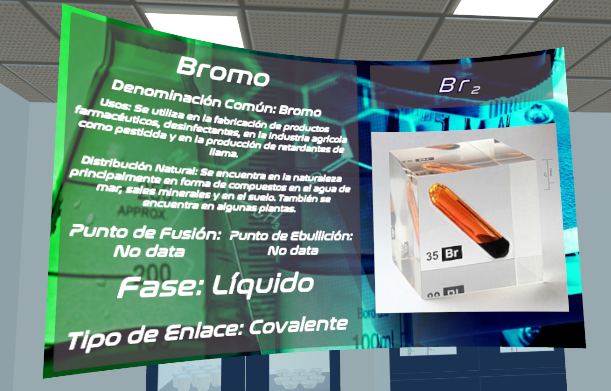
\includegraphics[width=0.6\textwidth, height = 6cm]{img/chapter04/UI_Compuestos.png}
    \caption{IU Compuestos}
    \label{fig:Compuestos_IU}
\end{figure}

\subsection{Área de creación}
Gestiona la combinación de elementos químicos.
\begin{itemize}
    \item \textbf{Indicador de contenido}: Lista dinámica de los elementos colocados en el área de creacón.
    \item \textbf{Validación automática}: Notificación visual que indica si la combinación es válida para generar un compuesto
    \item \textbf{Botón Crear}: Activo únicamente cuando los elementos combinados forman un compuesto válido. Al presionarlo, se genera el compuesto y se actualiza la interfaz.
\end{itemize}
\begin{figure}[thbp]
    \centering
    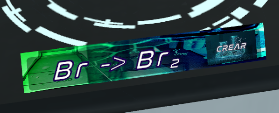
\includegraphics[width=0.6\textwidth, height = 6cm]{img/chapter04/UI_Creacion.png}
    \caption{IU Creación}
    \label{fig:Creación_IU}
\end{figure}
\newpage
\subsection{Teclado numérico interactivo}
Se sincroniza con las ecuaciones químicas mostradas en la IU de información principal, permitiendo la edición en tiempo real.
\begin{figure}[thbp]
    \centering
    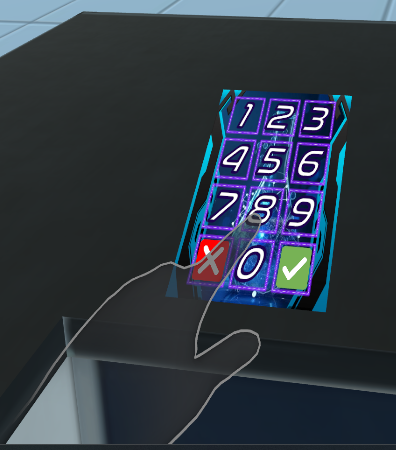
\includegraphics[width=0.4\textwidth, height = 6cm]{img/chapter04/Num_Pad.png}
    \caption{IU Numpad}
    \label{fig:Numpad_IU}
\end{figure}
\subsection{Pantalla final}
Marca la conclusión de un experimento e incluye dos acciones clave:
\begin{itemize}
    \item Repetir experimento: Reinicia el procedimiento desde el principio.
    \item Regresar al hub inicial: Permite al usuario explorar otras opciones o finalizar la sesión.
\end{itemize}
\begin{figure}[thbp]
    \centering
    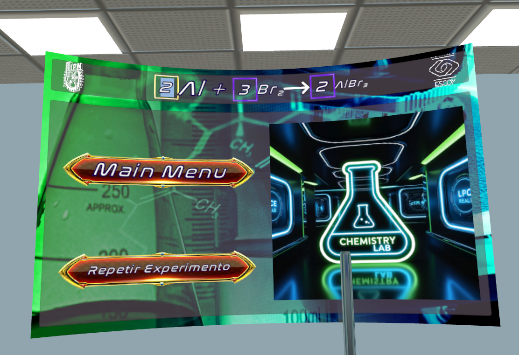
\includegraphics[width=0.6\textwidth, height = 6cm]{img/chapter04/UI_Final.png}
    \caption{IU Pantalla Final}
    \label{fig:Final_IU}
\end{figure}
\newpage
\section{Interacción y Gestos}\label{sec:Gestos}
La interacción dentro del simulador se diseñó para aprovechar las capacidades del seguimiento de manos (hand tracking) ofrecidas por el SDK de Oculus. Esto permite una experiencia intuitiva y natural para el usuario, integrando gestos básicos que emulan acciones físicas reales y simplifican la navegación en el entorno virtual.

\subsection{Interacción con el sistema}
Gracias a las herramientas proporcionadas por el SDK de Oculus, los objetos interactivos fueron configurados con los scripts Grabbable y Hand Grab Interactable. Esto habilita dos formas principales de interacción con los objetos en el entorno:

\begin{itemize}
    \item Sujeción completa: El usuario puede interactuar con los objetos cerrando completamente su mano alrededor de ellos, replicando la acción física de sujetar un objeto.
    \begin{figure}[thbp]
        \centering
        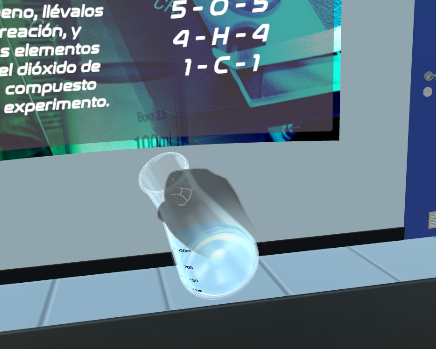
\includegraphics[width=0.6\textwidth, height = 6cm]{img/chapter04/Sujeción_Completa.png}
        \caption{Sujeción completa}
        \label{fig:Sujeción_Completa}
    \end{figure}
    \item Gesto de pinchar: El usuario junta el dedo índice y el pulgar (gesto de pinchar) para manipular objetos más pequeños o realizar interacciones precisas, como seleccionar botones o modificar valores.
    \begin{figure}[thbp]
        \centering
        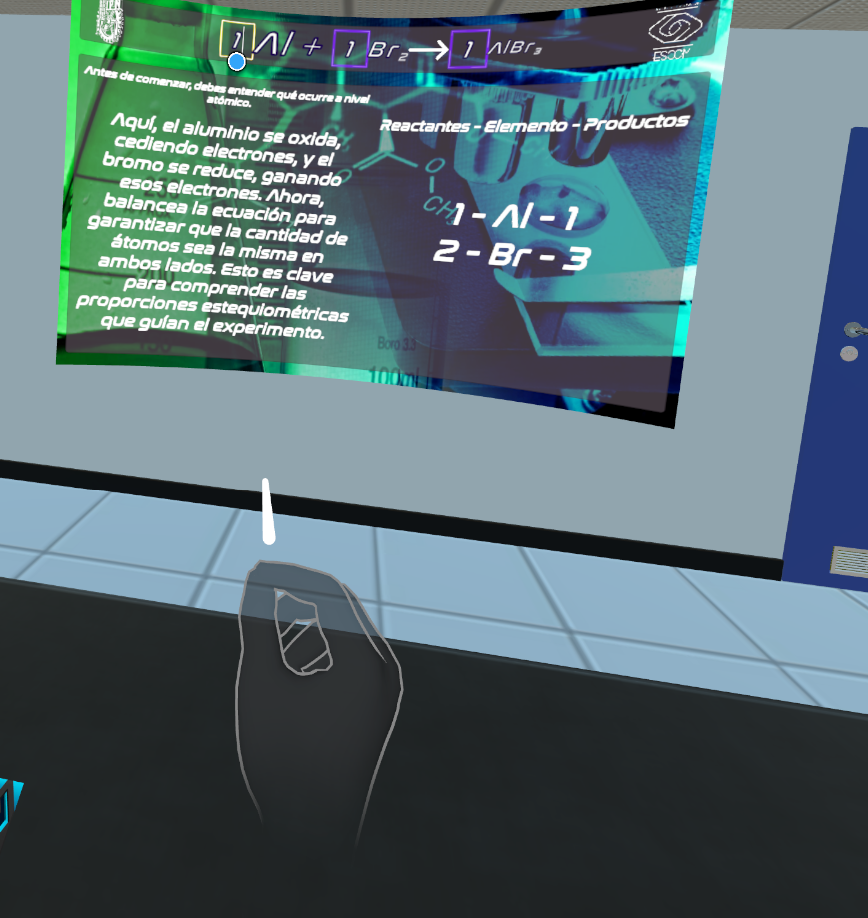
\includegraphics[width=0.6\textwidth, height = 6cm]{img/chapter04/Pinch.png}
        \caption{Gesto de pinchar}
        \label{fig:Pinchar}
    \end{figure}
\end{itemize}

Este gesto específico también se utiliza para interactuar con coeficientes en las ecuaciones químicas y en la selección de botones mediante un apuntador virtual. Esto asegura que las interacciones sean ergonómicas y precisas, incluso en actividades detalladas.

\subsection{Gestos específicos}
Se implementaron gestos adicionales para optimizar la interacción con el laboratorio:
\begin{itemize}
    \item Selección directa con el dedo índice: Al tocar directamente la tabla periódica interactiva o botones cercanos, el sistema reconoce el contacto del dedo índice y activa la acción correspondiente. Esto elimina la necesidad de punteros adicionales para elementos de acceso rápido.
    \begin{figure}[thbp]
        \centering
        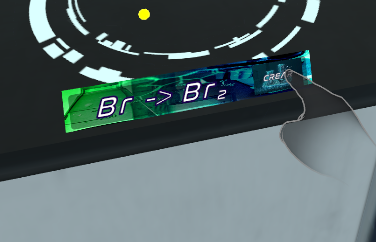
\includegraphics[width=0.6\textwidth, height = 6cm]{img/chapter04/Botones_Cercanos.png}
        \caption{Interacción con botones cercanos}
        \label{fig:Interacción}
    \end{figure}
    \item Centrado del escenario: Se habilitó un gesto general estándar de Oculus para centrar el entorno a la vista del usuario. Este gesto garantiza que el laboratorio virtual se ajuste correctamente al campo de visión, mejorando la comodidad y la orientación espacial del usuario.
    \begin{figure}[thbp]
        \centering
        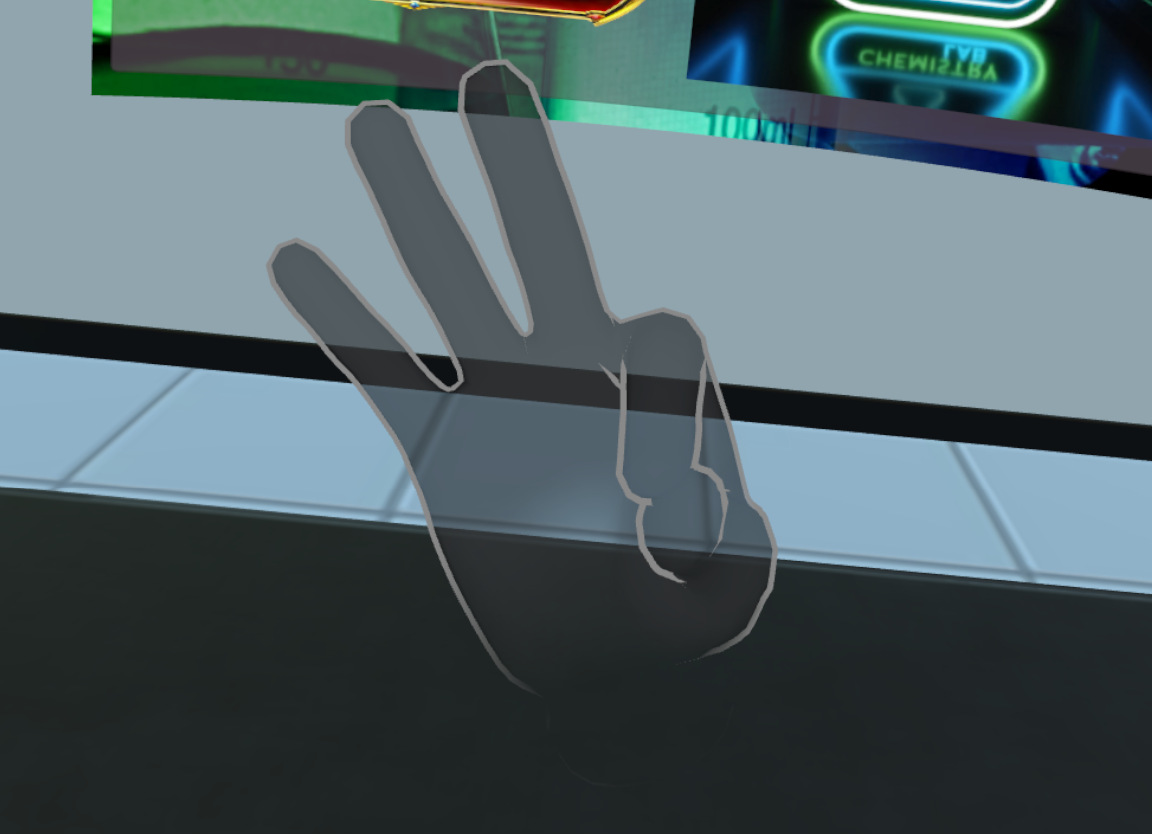
\includegraphics[width=0.6\textwidth, height = 6cm]{img/chapter04/Centrado.png}
        \caption{Gesto para centrar el entorno}
        \label{fig:Centrar}
    \end{figure}
\end{itemize}
El uso de gestos básicos asegura que los usuarios puedan interactuar con el entorno sin requerir controladores físicos. Esto reduce la curva de aprendizaje y mejora la experiencia inmersiva.
\newpage
\section{Integración del SDK de Oculus}
El desarrollo del simulador requirió la implementación del SDK de Oculus, una herramienta clave para habilitar capacidades de realidad virtual inmersiva. Este SDK proporciona un modelo completo que integra cámaras virtuales, controladores y seguimiento de manos (hand tracking) en un entorno preconfigurado.

Para este proyecto, se utilizó el módulo de hand tracking como base principal de interacción, aprovechando su capacidad para detectar y procesar movimientos naturales de las manos sin necesidad de controladores físicos. Este enfoque es particularmente relevante para la interacción con objetos y elementos virtuales descritos en la \autoref{sec:Ambiente_Virtual}: Ambiente Virtual y la \autoref{sec:Gestos}: Interacción y Gestos.

La integración del SDK de Oculus simplificó significativamente el desarrollo del simulador, proporcionando una base sólida para implementar las interacciones y funcionalidades principales sin necesidad de construir estas capacidades desde cero.
    \chapter{Implementación}\label{ch:Implementación}

En este capítulo se describen las principales escenas que componen el simulador, las máquinas de estado que gestionan el flujo de cada una, las acciones que los usuarios pueden realizar, y los scripts más relevantes que soportan la funcionalidad del sistema. El simulador está diseñado para guiar al usuario a través de una experiencia educativa interactiva y estructurada, permitiendo un aprendizaje inmersivo en el contexto de un laboratorio de química inorgánica.

\section{Fases de los Experimentos}
Los experimentos en el simulador están estructurados en cinco fases principales, cada una diseñada para facilitar la comprensión y ejecución de los procesos químicos involucrados. Estas fases aseguran que el usuario avance de manera lógica y progresiva, consolidando conocimientos y habilidades a lo largo de la actividad.

\subsection{Introducción}
En esta fase inicial, se da la bienvenida al usuario con una explicación clara del experimento y sus objetivos principales. Se destaca el contexto químico de la actividad, los materiales necesarios, y una descripción breve pero detallada del fenómeno que se observará. Esta etapa motiva al usuario y establece las bases para comprender los conceptos químicos que serán explorados durante el experimento.
\subsection{Balanceo de Ecuaciones}
El usuario aprende sobre las reacciones químicas involucradas en el experimento a través del análisis y balanceo de ecuaciones. Se le proporciona una ecuación inicial que deberá balancear para garantizar que la cantidad de átomos en ambos lados sea equivalente. El sistema guía al usuario paso a paso, explicando los conceptos básicos y proporciones estequiométricas, mientras utiliza el teclado numérico interactivo para ingresar los coeficientes correctos.
\subsection{Selección y Creación}
El usuario selecciona los elementos necesarios desde la tabla periódica virtual y los combina en el área de creación para formar los compuestos requeridos. A través de gestos intuitivos, como el de pinchar o agarrar, se seleccionan materiales como líquidos o sólidos, que luego se transforman en objetos interactivos listos para el experimento. El sistema proporciona retroalimentación visual para indicar que los compuestos se han preparado correctamente antes de proceder a la experimentación.
\subsection{Experimentación}
En esta etapa, el usuario lleva a cabo el experimento siguiendo instrucciones precisas y detalladas. Se realizan acciones como agregar líquidos o sólidos a recipientes, encender un mechero, calentar materiales, o combinar reactivos, observando los cambios físicos y químicos en tiempo real. Cada acción está respaldada por efectos visuales y sonoros que simulan fenómenos como la liberación de gases, formación de humo, cambios de color y producción de calor o luz, creando una experiencia inmersiva y educativa.
\subsection{Explicación}
Finalmente, el usuario recibe una explicación detallada de los resultados obtenidos durante el experimento. Esta fase resalta los principios químicos involucrados, como reacciones redox, formación de compuestos o cambios energéticos. Se utilizan gráficos y representaciones visuales para reforzar el aprendizaje, asegurando que el usuario comprenda plenamente el fenómeno observado y su relevancia en el contexto de la química.
\newpage
\section{Escenas Principales}
\subsection{Hub}
En la escena del Hub, se implementó una máquina de estados finita (FSM) para gestionar las transiciones entre las diferentes opciones disponibles, como el acceso al tutorial o a los experimentos. Este diseño permite una navegación fluida y estructurada, asegurando que el usuario pueda seleccionar y avanzar hacia las actividades deseadas de manera eficiente.

\begin{figure}[thbp]
    \centering
    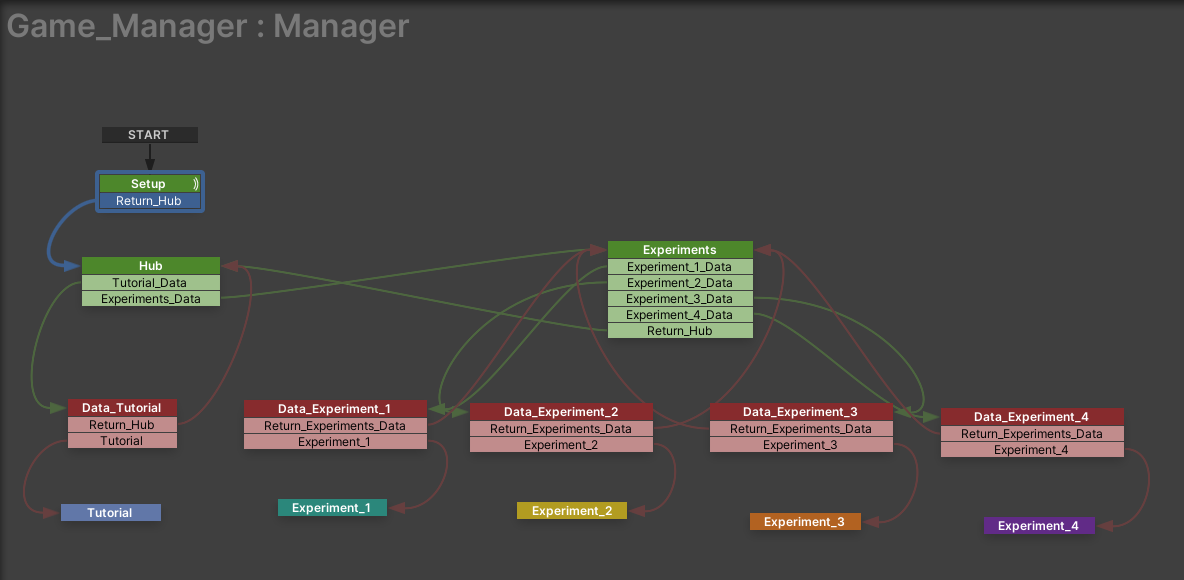
\includegraphics[width=0.7\textwidth, height = 7cm]{img/chapter05/Hub.png}
    \caption{Flujo de la escena Hub}
    \label{fig:FSM_Hub}
\end{figure}

Para implementar y manejar esta máquina de estados, se utilizó el script \texttt{MenuController}, que se encuentra detallado en la (\autoref{script:MenuController}). Este script es responsable de la lógica principal, como el manejo de eventos, la actualización de datos en la interfaz y la ejecución de las transiciones correspondientes dentro del flujo definido por la FSM.
La \autoref{fig:FSM_Hub} muestra el diagrama de la máquina de estados que estructura esta escena.

\subsection{Tutorial}
La escena de Tutorial utiliza una FSM para organizar las etapas de aprendizaje, desde la introducción hasta la realización de interacciones clave. Esta máquina guía al usuario a través de un proceso secuencial diseñado para familiarizarlo con las mecánicas del simulador y las herramientas virtuales.
\begin{figure}[thbp]
    \centering
    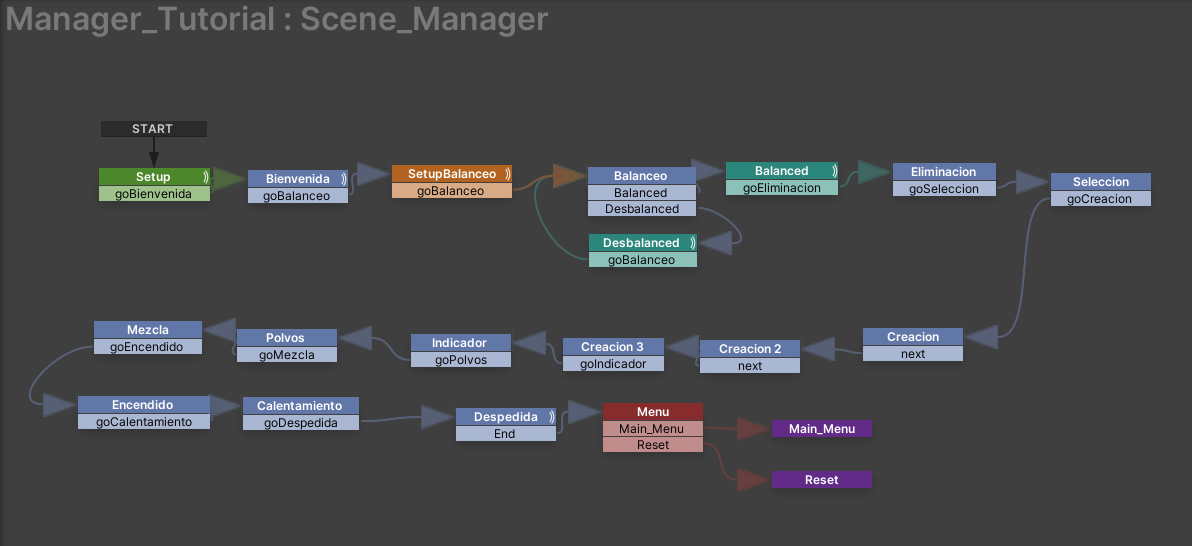
\includegraphics[width=0.7\textwidth, height = 7cm]{img/chapter05/Tutorial.png}
    \caption{Flujo de la escena Tutorial}
    \label{fig:FSM_Tutorial}
\end{figure}

La escena comienza con una bienvenida que introduce al usuario a las herramientas y conceptos básicos del simulador. Luego, se presentan tareas prácticas que incluyen el balanceo de ecuaciones, la selección y mezcla de sustancias, y el encendido y calentamiento de materiales, todo respaldado por retroalimentación visual y auditiva. Finalmente, la escena concluye con una despedida que refuerza los conceptos aprendidos y permite al usuario volver al menú principal.
\newpage
\subsection{Experimento 1}
La escena del Experimento 1 está diseñada para gestionar tareas específicas relacionadas con el balanceo de ecuaciones químicas y la manipulación de sustancias. La FSM controla cada etapa del experimento, permitiendo avanzar solo cuando las condiciones necesarias se cumplen.
\begin{figure}[thbp]
    \centering
    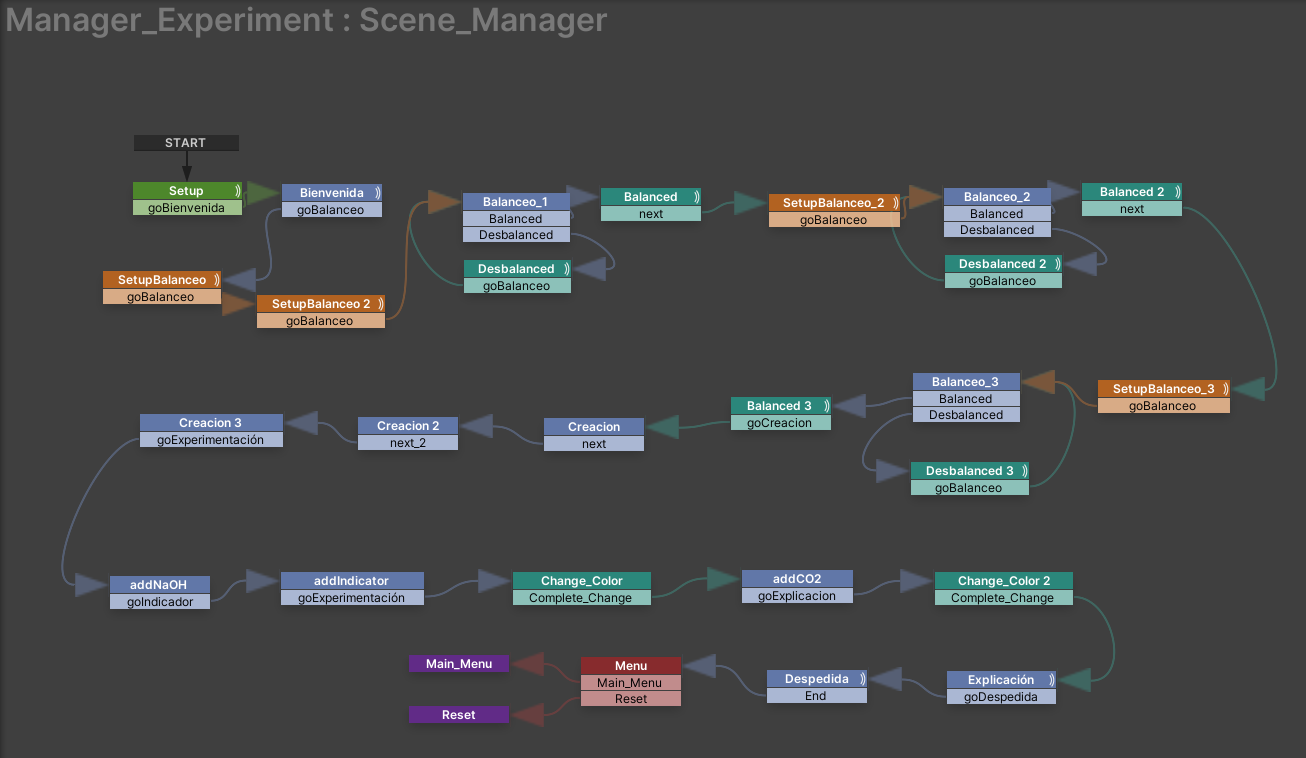
\includegraphics[width=0.7\textwidth, height = 7cm]{img/chapter05/Experimento_01.png}
    \caption{Flujo de la escena Experimento 1}
    \label{fig:FSM_E1}
\end{figure}

El flujo del experimento incluye pasos como el balanceo de ecuaciones químicas, la selección de sustancias específicas y su combinación, y la observación de cambios visuales en los materiales. Cada etapa está respaldada por retroalimentación visual y auditiva para mejorar la comprensión del usuario. Además, se utilizan efectos visuales, como cambios de color, para simular reacciones químicas.

El script \texttt{Experiment\_1\_Manager}, documentado en la \autoref{script:Experiment1Manager} valida las acciones del usuario, como la correcta combinación de sustancias, y activa eventos en la FSM para reflejar el progreso en tiempo real. Además, se manejan efectos visuales para representar las reacciones químicas de forma precisa. La estructura del flujo de esta escena se puede observar en la \autoref{fig:FSM_E1}.

\subsection{Experimento 2}
En el Experimento 2, la FSM organiza actividades que involucran la validación de mezclas químicas y la manipulación de temperatura. Los estados aseguran que las condiciones del experimento, como el tiempo de calentamiento o las combinaciones correctas, se cumplan antes de proceder.
\begin{figure}[thbp]
    \centering
    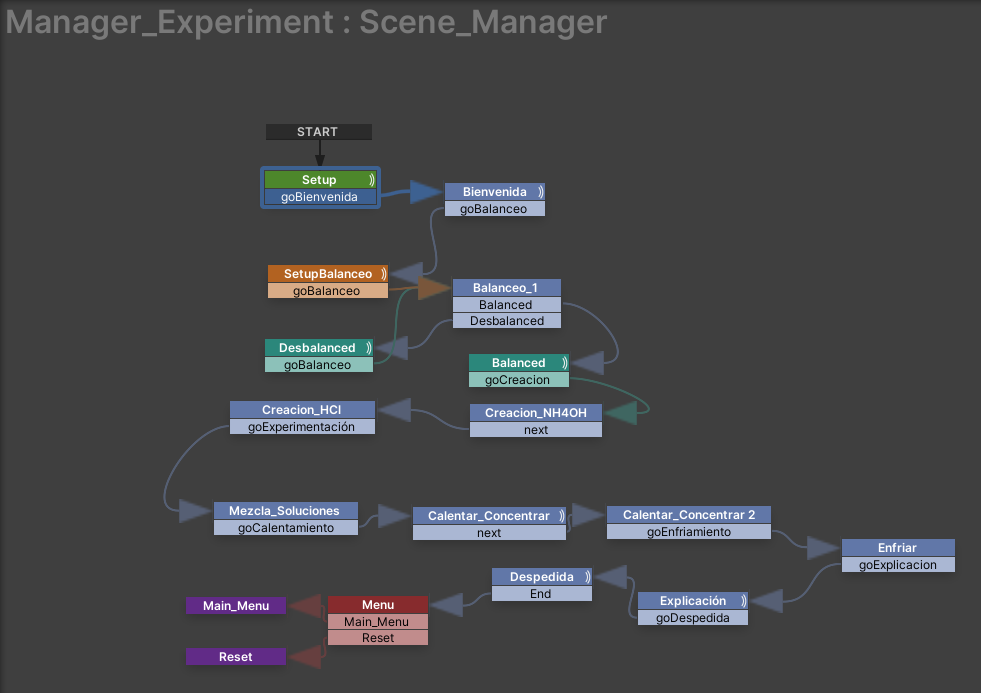
\includegraphics[width=0.7\textwidth, height = 7cm]{img/chapter05/Experimento_02.png}
    \caption{Flujo de la escena Experimento 2}
    \label{fig:FSM_E2}
\end{figure}

El script \texttt{Experiment\_2\_Manager}, documentado en la \autoref{script:Experiment2Manager}, implementa la lógica para monitorear estos parámetros y activar transiciones en la FSM, además de generar efectos visuales y auditivos que simulan las reacciones químicas.

\subsection{Experimento 3}
La FSM del Experimento 3 gestiona las combinaciones de sustancias y la activación de reacciones exotérmicas, estructurando el flujo del experimento para garantizar que cada acción del usuario sea validada antes de avanzar.
\begin{figure}[thbp]
    \centering
    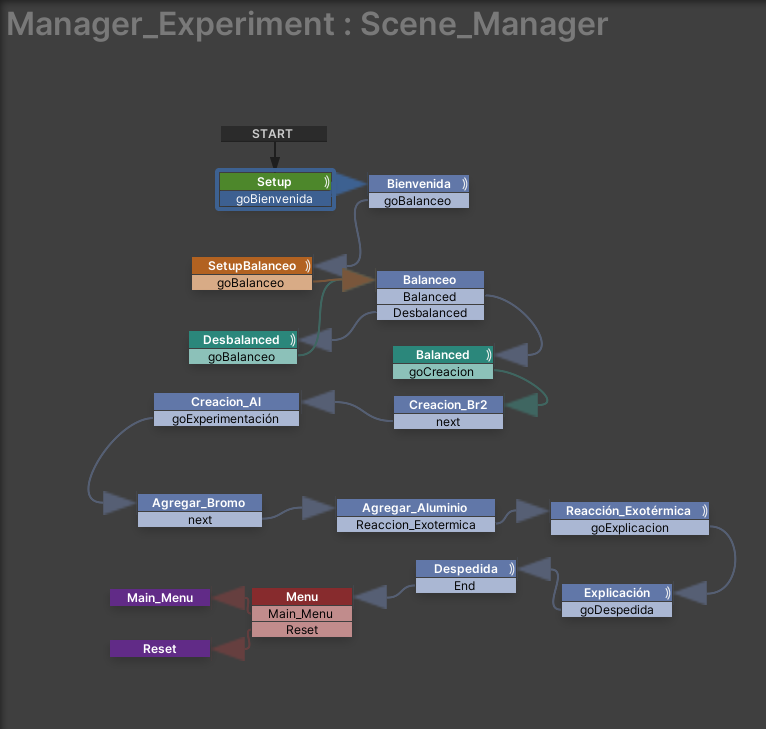
\includegraphics[width=0.7\textwidth, height = 7cm]{img/chapter05/Experimento_03.png}
    \caption{Flujo de la escena Experimento 3}
    \label{fig:FSM_E3}
\end{figure}

El script \texttt{Experiment\_3\_Manager}, documentado en la \autoref{script:Experiment3Manager}, se encarga de verificar las combinaciones realizadas y de controlar eventos visuales, como el llenado de recipientes, ofreciendo una experiencia interactiva y alineada con los objetivos del experimento.

\subsection{Experimento 4}
El Experimento 4 utiliza una FSM para gestionar tareas relacionadas con la manipulación de magnesio y dióxido de carbono sólido (hielo seco). Las etapas incluyen la preparación inicial, el encendido del magnesio, y la observación de una reacción exotérmica que genera luz intensa y subproductos químicos.
\begin{figure}[thbp]
    \centering
    \includegraphics[width=0.7\textwidth, height = 7cm]{img/chapter05/Experimento_04.png}
    \caption{Flujo de la escena Experimento 4}
    \label{fig:FSM_E4}
\end{figure}

El script \texttt{Experiment\_4\_Manager}, documentado en la \autoref{script:Experiment4Manager},  valida las acciones del usuario, como la correcta combinación de sustancias, y coordina eventos visuales y auditivos que simulan los procesos químicos involucrados. Este enfoque asegura que la experiencia sea inmersiva y técnicamente precisa.
\newpage
\section{Acciones del Usuario}
En el simulador, los usuarios tienen la capacidad de interactuar con diversos elementos y realizar acciones que son esenciales para completar los experimentos. Estas interacciones están diseñadas para ser intuitivas y están respaldadas por un sistema de lógica basado en máquinas de estados y scripts específicos que controlan los flujos de acción. A continuación, se describen las principales acciones disponibles.
\subsection{Manipulación de Objetos}
El usuario puede tomar objetos interactuables, como recipientes, herramientas de laboratorio y materiales, utilizando los gestos configurados con el SDK de Oculus. 
\begin{figure}[thbp]
    \centering
    \begin{subfigure}[b]{0.4\linewidth}
        \includegraphics[width=\linewidth, height = 5cm]{img/chapter05/Manipulación_01.png}
    \end{subfigure}
    \begin{subfigure}[b]{0.4\linewidth}
        \includegraphics[width=\linewidth, height = 5cm]{img/chapter05/Pinch (2).png}
    \end{subfigure}
    \begin{subfigure}[b]{0.4\linewidth}
        \includegraphics[width=\linewidth, height = 5cm]{img/chapter05/Agarre.png}
    \end{subfigure}
    \caption{Diversas Interacciones con objetos}
\end{figure}
\newpage
\subsection{Selección de Elementos en la Tabla Periódica}
El simulador incluye una tabla periódica interactiva donde el usuario puede seleccionar elementos químicos con un gesto de toque directo. Los elementos seleccionados se transforman en sus representaciones virtuales (modelos atómicos o sustancias químicas) y pueden ser llevados al área de creación o al experimento.
\begin{figure}[thbp]
    \centering
    \includegraphics[width=0.6\textwidth, height = 5cm]{img/chapter05/Tabla_Periodica.png}
    \caption{Tabla Periódica}
    \label{fig:Tabla_Periódica}
\end{figure}
\subsection{Creación y Manipulación de Compuestos}
Los compuestos químicos se generan combinando elementos o materiales en áreas específicas designadas. El sistema valida automáticamente las combinaciones correctas y actualiza el estado de los experimentos, proporcionando retroalimentación visual y textual sobre el progreso.
\begin{figure}[thbp]
    \centering
    \includegraphics[width=0.7\textwidth, height = 7cm]{img/chapter05/Zona_Creación (2).png}
    \caption{Zona de Creación de compuestos}
    \label{fig:Creación_Compuestos}
\end{figure}
\newpage
\subsection{Encendido de Mecheros y Materiales}
El encendido se realiza al acercar la flama del encendedor al mechero o a algún compuesto que deba quemarse. Una vez que el encendedor está lo suficientemente cerca, el sistema detecta la proximidad y activa la acción correspondiente, generando los efectos visuales y sonoros que simulan la ignición.
\begin{figure}[thbp]
    \centering
    \begin{subfigure}[b]{0.3\linewidth}
        \includegraphics[width=\linewidth, height = 5cm]{img/chapter05/Encendido01.png}
        \caption{Uso de encendedor}
        \label{fig:Encendedor}
    \end{subfigure}
    \begin{subfigure}[b]{0.3\linewidth}
        \includegraphics[width=\linewidth, height = 5cm]{img/chapter05/Encendido02.png}
        \caption{Encendido de mechero}
        \label{fig:Mechero}
    \end{subfigure}
    \begin{subfigure}[b]{0.3\linewidth}
        \includegraphics[width=\linewidth, height = 5cm]{img/chapter05/Encendido03.png}
        \caption{Encendidos de material}
        \label{fig:Material_Encendido}
    \end{subfigure}
    \caption{Encendido diverso}
\end{figure}
\subsection{Eliminación de Elementos}
Para eliminar un elemento seleccionado, el usuario debe llevarlo a la zona de desecho. Una vez en esta área, el sistema lo detecta y elimina automáticamente, permitiendo mantener un espacio de trabajo ordenado y sin materiales innecesarios.
\begin{figure}[thbp]
    \centering
    \includegraphics[width=0.7\textwidth, height = 7cm]{img/chapter05/Eliminación.png}
    \caption{Eliminación de un elemento}
    \label{fig:Eliminación}
\end{figure}
\newpage
\subsection{Acciones Relacionadas con Líquidos}
Las interacciones con líquidos están diseñadas para ser inmersivas y detalladas, permitiendo al usuario:
\begin{figure}[thbp]
    \centering
    \includegraphics[width=0.7\textwidth, height = 7cm]{img/chapter05/Liquids.png}
    \caption{FSM Comportamiento de Liquidos}
    \label{fig:FSM_Liquids}
\end{figure}
\begin{itemize}
    \item Calentar líquidos: Al colocar un recipiente en un trípode con rejilla por encima de un mechero encendido, el líquido comienza a calentarse de manera progresiva. Este proceso está acompañado de efectos visuales como burbujeo y generación de vapor, que simulan las propiedades físicas reales del calentamiento.
    
    El estado del calentamiento se gestiona mediante la FSM correspondiente, que controla las transiciones entre los estados como ``Heating'' o ``PreWarm", dependiendo de la proximidad del recipiente al mechero y el tiempo de exposición al calor (ver \autoref{fig:FSM_Liquids}).
    \item Transferencia de líquidos entre recipientes: Los usuarios pueden verter líquidos de un recipiente a otro inclinando el primero, lo que activa estados como ``Spilling'' o ``Filling''. Estas acciones generan efectos visuales de derrame y llenado, junto con la actualización dinámica del nivel del líquido en ambos recipientes.
    \item Agregar sólidos a líquidos: La adición de polvos o sólidos genera reacciones químicas específicas, con cambios visuales como efervescencia o cambios de color, dependiendo del experimento.
\end{itemize}
\begin{figure}[thbp]
    \centering
    \begin{subfigure}[b]{0.3\linewidth}
        \includegraphics[width=\linewidth, height = 4cm]{img/chapter05/Calentamiento.png}
        \caption{Calentamiento de Líquidos}
        \label{fig:Calentamiento}
    \end{subfigure}
    \begin{subfigure}[b]{0.3\linewidth}
        \includegraphics[width=\linewidth, height = 4cm]{img/chapter05/Vertido.png}
        \caption{Transferencia de Líquidos}
        \label{fig:Vertido}
    \end{subfigure}
    \begin{subfigure}[b]{0.3\linewidth}
        \includegraphics[width=\linewidth, height = 4cm]{img/chapter05/Agregar_Solidos.png}
        \caption{Interacción con Sólidos}
        \label{fig:Sólidos}
    \end{subfigure}
    \caption{Diversas Interacciones de Líquidos}
\end{figure}

    \chapter{Presentaciones y Pruebas del Prototipo}\label{ch:Pruebas}
A lo largo del año de desarrollo, el prototipo del simulador fue presentado en diversos eventos e instituciones, lo que permitió recopilar retroalimentación clave para optimizar su funcionalidad y experiencia de usuario. Además, estas pruebas y presentaciones sirvieron para validar la precisión química de las reacciones y procesos representados, en colaboración con especialistas en el área.

\section{Presentaciones Institucionales}
El simulador fue exhibido como parte de las actividades de difusión del \textbf{Centro de Innovación y Desarrollo Tecnológico (CIDETEC) del Instituto Politécnico Nacional (IPN)}. Estas presentaciones estuvieron dirigidas a grupos invitados de diversas universidades e instituciones educativas, que tuvieron la oportunidad de observar y probar el prototipo. Entre las instituciones participantes se encuentran:
\begin{itemize}
    \item Tecnológico de Estudios Superiores de Jocotitlán\\
    Fecha: 24 de mayo de 2024.
    \item ESIME-Culhuacán, IPN\\
    Fecha: 7 de junio de 2024.
    \item UPIIZ, IPN\\
    Fechas: 21 de junio de 2024 y 27 de septiembre de 2024.
    \item Universidad Tecnológica de Xicotepec de Juárez\\
    Fecha: 5 de julio de 2024.
    \item Universidad Mexiquense del Bicentenario\\
    Fecha: 18 de octubre de 2024.
\end{itemize}
\begin{figure}[thbp]
    \centering
    \includegraphics[width=0.7\textwidth, height = 7cm]{img/chapter06/CIDETEC.jpg}
    \caption{Presentaciones Institucionales}
    \label{fig:CIDETEC}
\end{figure}
Estas presentaciones permitieron recopilar observaciones de estudiantes en un entorno controlado, ayudando a identificar oportunidades de mejora y ajustar detalles técnicos del simulador.
\newline
\section{Invitaciones Externas}
Además de las presentaciones institucionales, el simulador fue invitado a participar en eventos externos y actividades organizadas por otras instituciones. Estas invitaciones ampliaron el alcance del proyecto y permitieron recibir retroalimentación de públicos diversos. Los eventos destacados incluyen:
\begin{itemize}
    \item \textbf{Centro de Estudios Superiores Isidro Fabela (Bachillerato)}\\
    Fecha: 13 de junio de 2024.
    \begin{figure}[thbp]
        \centering
        \includegraphics[width=0.5\textwidth, height = 5cm]{img/chapter06/CESIF_01.jpg}
        \caption{Presentación Isidro Fabela}
        \label{fig:CESIF}
    \end{figure}
    \newpage
    \item \textbf{Cinvesniños, CINVESTAV - IPN}\\
    Fechas: 22 y 23 de noviembre de 2024, en el stand  ``Uso de la realidad virtual en la ciencia''. Este fue el único evento público abierto, en el que participaron niños, jóvenes y adultos, ofreciendo perspectivas variadas sobre la accesibilidad y el impacto educativo del simulador.
    \begin{figure}[thbp]
        \centering
        \begin{subfigure}{0.45\linewidth}
            \includegraphics[width=\linewidth, height = 5cm]{img/chapter06/CINVESTAV_02.jpg}
        \end{subfigure}
        \begin{subfigure}{0.45\linewidth}
            \includegraphics[width=\linewidth, height = 5cm]{img/chapter06/CINVESTAV_03.jpg}
        \end{subfigure}
        \caption{Presentación en Cinvesniños}
    \end{figure}
    \item \textbf{Universidad Estatal del Valle de Ecatepec}\\
    Fecha: 27 de noviembre de 2024.
    \begin{figure}[thbp]
        \centering
        \begin{subfigure}{0.45\linewidth}
            \includegraphics[width=\linewidth, height = 5cm]{img/chapter06/UEVE.png}
        \end{subfigure}
        \begin{subfigure}{0.45\linewidth}
            \includegraphics[width=\linewidth, height = 5cm]{img/chapter06/UEVE.jpg}
        \end{subfigure}
        \caption{Presentación UEVE}
    \end{figure}
\end{itemize}
\newpage
\section{Colaboración y Validación Académica}
Durante el desarrollo del proyecto, se contó con el apoyo de la Escuela Secundaria Diurna No. 4 ``Moisés Sáenz'' y del profesor Ernesto Uribe. Este trabajo conjunto incluyó sesiones de prueba con estudiantes y reuniones privadas para afinar detalles técnicos y validar la precisión de las reacciones químicas y los procesos educativos mostrados en el simulador.

Las pruebas realizadas con los estudiantes ayudaron a evaluar la usabilidad y la experiencia del usuario, mientras que las reuniones con el profesor permitieron garantizar la exactitud y la relevancia de la información química representada en el sistema.
\begin{figure}[thbp]
    \centering
    \begin{subfigure}{0.45\linewidth}
        \includegraphics[width=\linewidth, height = 5cm]{img/chapter06/Sec_02.jpg}
    \end{subfigure}
    \begin{subfigure}{0.45\linewidth}
        \includegraphics[width=\linewidth, height = 5cm]{img/chapter06/Sec_08.jpg}
    \end{subfigure}
    \begin{subfigure}{0.45\linewidth}
        \includegraphics[width=\linewidth, height = 5cm]{img/chapter06/Sec_05.jpg}
    \end{subfigure}
    \caption{Reuniones en Secundaria 4}
\end{figure}
    \chapter{Conclusiones}\label{ch:Conclusiones}
El desarrollo del prototipo de simulador de laboratorio de química inorgánica en realidad virtual permitió abordar una necesidad educativa específica mediante una herramienta tecnológica innovadora. A pesar de la existencia de otros simuladores en el ámbito de la química, muchos carecen de una experiencia inmersiva y altamente interactiva. Además, pocos están diseñados específicamente para un público mexicano, limitando su aplicabilidad y efectividad en contextos educativos locales.

El prototipo desarrollado logró implementar cuatro experimentos y un tutorial, permitiendo la realización de prácticas químicas con un nivel aceptable de precisión. Este sistema se centró en representar de manera detallada los aspectos visuales y físicos de las reacciones químicas.
Dichos elementos no solo enriquecen la experiencia del usuario, sino que también contribuyen significativamente a la comprensión de los procesos químicos involucrados.

Una de las características distintivas del simulador es su capacidad para emular experimentos comúnmente realizados en aulas de nivel secundaria. Esta funcionalidad permite a los usuarios interactuar con los experimentos en un entorno virtual, ofreciendo la posibilidad de comparar sus experiencias prácticas en entornos reales. De este modo, el prototipo fomenta un aprendizaje visual, interactivo e inmersivo, que apoya el proceso de enseñanza de conceptos químicos de manera efectiva.

El desarrollo del prototipo presentó retos técnicos y multidisciplinarios, ya que involucró áreas como la química, la enseñanza, el desarrollo de software, el diseño y modelado 3D, y la implementación de tecnologías de realidad virtual. Si bien la creación de los módulos fue compleja, gran parte del esfuerzo se destinó a superar la curva de aprendizaje asociada al enfoque innovador del proyecto.

Finalmente, se concluye que los objetivos establecidos al inicio del proyecto fueron alcanzados. El prototipo cumple con el alcance planteado, al integrar un conjunto de experimentos funcionales, validados por un profesional en química, garantizando así la exactitud de los contenidos. El simulador ofrece una herramienta educativa inmersiva y funcional que puede adaptarse y escalarse en futuras iteraciones para seguir mejorando la enseñanza de la química.
    \chapter{Trabajo a Futuro}\label{ch:Trabajo_Futuro}
El prototipo desarrollado presenta un punto de partida sólido para la enseñanza inmersiva de la química inorgánica. Sin embargo, se han identificado áreas clave que podrían ser abordadas en futuras iteraciones para ampliar su funcionalidad, mejorar su impacto educativo y adaptarse a un público más amplio.
\begin{enumerate}[I.]
    \item \textbf{Ampliación del Catálogo de Experimentos}\\
    Actualmente, el simulador incluye cuatro experimentos básicos. Un paso importante a futuro sería la incorporación de nuevos experimentos que abarquen conceptos avanzados de química, incluyendo experimentos que involucren química orgánica o reacciones más complejas. Esto permitiría que el simulador sea útil no solo en el nivel secundaria, sino también en niveles educativos más avanzados, como bachillerato o universidad.
    \item \textbf{Evaluación del Aprendizaje}\\
    Integrar un sistema de evaluación del aprendizaje proporcionaría una retroalimentación inmediata sobre el desempeño de los usuarios. Esto podría incluir cuestionarios al final de cada experimento, análisis de las decisiones tomadas durante las prácticas y la generación de reportes de progreso. Un sistema de este tipo no solo reforzaría el aprendizaje, sino que también permitiría a los docentes medir el impacto del simulador en el desarrollo de habilidades químicas en los estudiantes.
    \item \textbf{Compatibilidad con Diversos Equipos de RV}\\
    Para ampliar el alcance del simulador, sería importante trabajar en la compatibilidad con una mayor variedad de dispositivos de realidad virtual, como Meta Quest, HTC Vive, o dispositivos más económicos que utilizan smartphones como visores. Esta flexibilidad tecnológica permitiría que más instituciones educativas, independientemente de sus recursos, puedan implementar el simulador en sus aulas.
    \item \textbf{Incorporación de Colaboración en Línea}\\
    El desarrollo de un modo multijugador o colaborativo en línea sería un avance significativo. Esto permitiría que varios usuarios trabajen juntos en experimentos en tiempo real, simulando prácticas grupales que son comunes en laboratorios físicos. Además, este enfoque fomentaría el aprendizaje cooperativo y permitiría la participación remota, haciendo el simulador accesible para estudiantes en ubicaciones geográficas distintas.
\end{enumerate}
Estas propuestas de trabajo a futuro buscan consolidar el simulador como una herramienta educativa avanzada y versátil, capaz de adaptarse a diversas necesidades y contextos. Su implementación podría transformar el prototipo en una plataforma integral para el aprendizaje de la química, 

    \appendix
        \chapter{Descripción Detallada de los Experimentos}\label{app:Experimentos}

\section{\textit{\textbf{De Básico a Ácido}}} 
\textit{\textsc{Cambio de pH al Añadir dióxido de carbono (\ch{CO2}) a una Solución de hidróxido de sodio (\ch{NaOH}) con Azul de Bromotimol }}

    \textit{\textbf{Introducción  }}
    
    El pH de una solución mide su acidez o basicidad. Un pH bajo indica que la solución es ácida, mientras que un pH alto indica que es básica. El indicador azul de bromotimol cambia de color dependiendo del pH:
    
    \begin{itemize}
        \item Azul en soluciones básicas (pH $>$ 7.6)
        \item Verde en soluciones neutras (pH $\approx$ 7.0)
        \item Amarillo en soluciones ácidas (pH $<$ 6.0)
    \end{itemize} 

    En este experimento, vamos a cambiar el pH de una solución añadiendo primero una base (\ch{NaOH}) para hacerla más básica, y luego introduciremos dióxido de carbono (\ch{CO2}) para que se convierta en ácida.
    
    \textit{\textbf{Objetivo  }}
    
    Observar y comprender el cambio en el pH de una solución básica preparada con hidróxido de sodio (\ch{NaOH}) mediante la adición de dióxido de carbono (\ch{CO2}), utilizando el indicador azul de bromotimol para identificar el cambio de básico a ácido.
    
    \textit{\textbf{Materiales y Reactivos  }}
    \begin{itemize}
        \item Matraz Erlenmeyer (250 ml)
        \item 100 ml de agua destilada
        \item Azul de bromotimol (indicador de pH)
        \item Solución de hidróxido de sodio (\ch{NaOH}) al 0.1 M
        \item Hielo seco (\ch{CO2} sólido) o una fuente de gas \ch{CO2}
        \item Pipeta o gotero
        \item Guantes y gafas de seguridad
    \end{itemize}
    \clearpage
    \textit{\textbf{Procedimiento Experimental  }}
    \begin{enumerate}
        \item \textbf{Preparación de la Solución Básica: }
        \begin{itemize}
            \item Vierte 100 ml de agua destilada en un Matraz Erlenmeyer.
            \item Agrega 2-3 gotas de azul de bromotimol. La solución debería volverse verde (pH neutro).
            \item Añade unas gotas de solución de NaOH (hidróxido de sodio al 0.1 M). Observa cómo el color cambia a azul, indicando que la solución es ahora básica.
        \end{itemize}
    
        \textbf{Ecuación Química  }
        \begin{center}
            \ch{Na2O + H2O -> 2 NaOH}
        \end{center}

        Un hidróxido se forma cuando un óxido metálico reacciona con agua.
        
        \item \textbf{Acidificación de la Solución con \ch{CO2}:}

        Añade un pequeño trozo de hielo seco (\ch{CO2} sólido) o introduce gas \ch{CO2} en la solución. Observa cómo el color de la solución cambia primero a verde y luego a amarillo.

        \textbf{Reacción de \ch{CO2} con Agua:}
        El \ch{CO2} se disuelve en agua formando ácido carbónico, lo que baja el pH:
        
        \begin{center}
            \ch{CO2 + H2O -> H2CO3}
        \end{center}
        
        El ácido carbónico se disocia en iones de hidrógeno (\ch{H+}) y bicarbonto (\ch{HCO3-}), lo que causa la acides de la solución;
        
        \begin{center}
            \ch{H2CO3 -> H+ + HCO3-}
        \end{center}

        Los protones (\ch{H+}) son responsables de la disminución del pH, lo que hace que la solución cambie a un color amarillo, indicando que ahora es ácida.
    \end{enumerate}
    \textit{\textbf{Explicación Química }}  

    En este experimento, el hidróxido de sodio (\ch{NaOH}) se disuelve en agua, creando una solución básica con un pH alto, lo cual se observa como un cambio a color azul en el indicador azul de bromotimol. Lueho, al añadir dióxido de carbono (\ch{CO2}), este se disuelve y reacciona con el agua para formar ácido carbónico (\ch{H2CO3}), el cual se disocia parcialmente, liberando iones \ch{H+} y disminuyendo el pH de la solución.

    Este cambio de pH, visible en el indicador que pasa de azul a amarillo, demuestra cómo el \ch{CO2} puede acidificar una solución básica mediante la formación de ácido.
    
    \textit{\textbf{Resultados }} 
    
    Registrar el tiempo transcurrido hasta el cambio de color en cada experimento. Analizar cómo las variaciones en la concentración y la temperatura afectan este tiempo.  

    \clearpage
    
    \textit{\textbf{Conclusiones}}  
    \begin{itemize}
        \item Se observó que, al agregar \ch{CO2} al agua, la solución pasó de ser básica (azul) a ácida (amarillo).
        \item El cambio de color del indicador azul de bromotimol demostró cómo el \ch{CO2} reduce el pH de la solución.
        \item Este experimento muestra cómo el dióxido de carbono puede acidificar una solución mediante la formación de ácido carbónico.
    \end{itemize}
    
    \textit{\textbf{Medidas de Seguridad }} 
    \begin{itemize}
        \item Usa guantes y gafas de seguridad para evitar el contacto con \ch{NaOH} y hielo seco.
        \item No manipules el hielo seco directamente, usa pinzas o guantes gruesos. 
        \item Trabaja en un área bien ventilada y no inhales el \ch{CO2} directamente.
        \item Desecha los restos de la práctica de acuerdo con las normas de seguridad del laboratorio.
    \end{itemize}

    \textit{\textbf{Cuestionario}} 
    \begin{enumerate}
        \item ¿Qué ocurrió con el color de la solución después de añadir \ch{NaOH}? ¿Por qué?
        \item ¿Por qué se formó ácido carbónico al agregar \ch{CO2} al agua?
        \item ¿Qué indica el cambio de color de azul a amarillo en la solución?
        \item ¿Cómo podría usar el dióxido de carbono para cambiar el pH en otros experimentos?
    \end{enumerate}
    \newpage
\section{\textit{\textbf{La lámpara de magnesio}}} 
\textit{\textsc{Combustión del Magnesio en Hielo Seco}}

    \textit{\textbf{Introducción}}  
    
    El magnesio es un metal altamente reactivo que puede arder incluso en ausencia de oxígeno atmosférico. En este experimento, se observará cómo el magnesio puede reaccionar con el dióxido de carbono sólido (hielo seco), un compuesto comúnmente utilizado como extintor de incendios. Esta reacción demuestra la alta posición del magnesio en la serie de reactividad, desplazando al carbono para formar óxido de magnesio y carbono elemental.  
    
    \textit{\textbf{Objetivos }} 
    \begin{itemize}
        \item Demostrar que el magnesio puede arder en ausencia de oxígeno molecular. 
    
        \item Analizar los productos de la combustión del magnesio en hielo seco.  
        
        \item Comprender la reactividad del magnesio frente al dióxido de carbono.
        
    \end{itemize}
    \textit{\textbf{Materiales y Reactivos }} 
    \begin{itemize}
        \item Bloque de hielo seco (\ch{CO2} sólido). 
    
        \item Soplete o mechero Bunsen.
        
        \item Cincel o herramienta para cavidades. 
        
        \item Pinzas resistentes al calor.
        
        \item Guantes térmicos.
        
        \item Gafas de seguridad.

        \item Pantalla de protección.

        \item Virutas o cinta de magnesio (aproximadamente 5 g).
    \end{itemize}
    \textit{\textbf{Procedimiento Experimental}}  
    \begin{enumerate}
        \item \textbf{Preparación del hielo seco}: Usa un cincel para hacer una cavidad en el bloque de hielo seco de aproximadamente 3 cm de profundidad y 3 cm de ancho. Reserva el material extraído para usarlo como tapa.  
    
        \item \textbf{Colocación del magnesio}: Introduce las virutas de magnesio en la cavidad sin llenarla completamente, dejando al menos 1 cm de espacio por encima del material. 
    
        \item \textbf{Encendido del magnesio}: Utilizando un soplete o mechero Bunsen, calienta el magnesio directamente hasta que se inicie la combustión.
        
        Coloca rápidamente el tapón de hielo seco sobre la cavidad para minimizar la entrada de aire. 
    
        \item \textbf{Observación de la reacción}: Observa cómo el magnesio arde con una luz brillante en el ambiente de dióxido de carbono sólido, produciendo una mezcla de óxido de magnesio (polvo blanco) y carbono elemental (polvo negro).

        \item \textbf{Finalización}: Permite que el residuo se enfríe antes de manipularlo.
    \end{enumerate}
    \textit{\textbf{Explicación Química}}  
    
    La reacción química entre el magnesio y el dióxido de carbono se puede representar con la ecuación:
    
    \begin{center}
        \ch{2 Mg + CO2 -> 2 MgO + C}  
    \end{center}
    
    El magnesio desplaza al carbono del dióxido de carbono debido a su mayor reactividad, formando óxido de magnesio (\ch{MgO}) como producto principal y carbono elemental (\ch{C}) como subproducto. Esto demuestra que el magnesio puede arder en condiciones donde el oxígeno no está disponible. 
    
    \textit{\textbf{Resultados }} 
    
    Durante el experimento, se observó que el magnesio arde intensamente con una luz blanca brillante incluso en ausencia de oxígeno, utilizando el dióxido de carbono sólido como fuente de oxidación. La combustión produjo chispas y partículas expulsadas por la sublimación del hielo seco, dejando como residuo un polvo blanco (óxido de magnesio) y partículas negras (carbono elemental), evidenciando la transformación química esperada. 
    
    \textit{\textbf{Conclusiones }} 
    
    El magnesio demostró ser un metal altamente reactivo capaz de oxidarse utilizando dióxido de carbono como agente oxidante, lo que valida su posición por encima del carbono en la serie de reactividad química. Este experimento refuerza el concepto de que el oxígeno no siempre es imprescindible para una combustión y destaca la capacidad del magnesio para desplazar al carbono, formando óxido de magnesio y carbono elemental como productos finales.
    
    \textit{\textbf{Medidas de Seguridad }} 
    \begin{itemize}
        \item \textbf{Hielo seco}: El hielo seco debe manipularse siempre con guantes térmicos y gafas de seguridad para evitar quemaduras por congelación. Evite el contacto directo con la piel o los ojos, y no almacene el hielo seco en contenedores herméticos o espacios confinados debido al riesgo de acumulación de dióxido de carbono gaseoso que puede causar asfixia o explosión.

        \item \textbf{Magnesio y llama}: El magnesio y su combustión presentan riesgos significativos de quemaduras y proyección de partículas incandescentes. Utilice una pantalla de seguridad, gafas protectoras, guantes resistentes al calor y asegúrese de mantener materiales inflamables alejados del área de trabajo. Evite mirar directamente a la luz intensa producida por la combustión del magnesio para proteger sus ojos.

        \item \textbf{General}: Trabaje siempre en un área ventilada y mantenga al público a una distancia mínima de 2-3 metros detrás de una pantalla de seguridad. Use equipo de protección personal como bata, guantes, gafas y asegúrese de contar con extintores cerca del área de trabajo. Supervise el experimento en todo momento y siga los protocolos de manejo seguro de sustancias químicas y equipos de laboratorio.
    \end{itemize}
    \newpage
\section{\textit{\textbf{Nieve Química}}} 
\textit{\textsc{Síntesis de Cloruro de Amonio a partir de Hidróxido de Amonio y Ácido Clorhídrico}}

    \textit{\textbf{Introducción }} 
    
    El cloruro de amonio (\ch{NH4Cl}) es una sal inorgánica con diversas aplicaciones industriales y científicas. En este experimento, se llevará a cabo su síntesis mediante la reacción de neutralización entre hidróxido de amonio (\ch{NH4OH}) en solución acuosa y ácido clorhídrico (\ch{HCl}) en solución acuosa. La reacción es exotérmica y produce cloruro de amonio sólido, que precipita en forma de cristales.  
    
    \textit{\textbf{Objetivos  }}
    \begin{itemize}
        \item Sintetizar cloruro de amonio a partir de hidróxido de amonio y ácido clorhídrico.  
    
        \item Observar la formación de cristales de cloruro de amonio como producto de la reacción.  
        
        \item Comprender el concepto de reacción de neutralización y su aplicación en la síntesis de sales.  
    \end{itemize}
    \textit{\textbf{Materiales y Reactivos  }}
    \begin{itemize}
        \item Solución de hidróxido de amonio ({\ch{NH4OH}) concentrada (28-30\%)  
    
        \item Solución de ácido clorhídrico (\ch{HCl}) concentrada (37\%)  
        
        \item Vaso de precipitados de 250 ml  
        
        \item Probeta graduada de 50 ml  
        
        \item Varilla de vidrio  
        
        \item Pipeta graduada 
    \end{itemize}
    \textit{\textbf{Procedimiento Experimental }} 
    \begin{enumerate}
        \item Preparación de las soluciones:  medir 32.4 ml de hidróxido de amonio concentrado con una probeta graduada y verterlos en un vaso de precipitados de 250 ml.  
        
        \item Medición del ácido clorhídrico: Medir 25 ml de ácido clorhídrico concentrado con una probeta graduada.  
        
        \item Reacción de neutralización: Lentamente y con precaución, agregar el ácido clorhídrico a la solución de hidróxido de amonio. Agitar suavemente la mezcla. Observar la formación de una densa nube blanca de cloruro de amonio sólido.  
        
        \item Concentración del soluto: Calentar suavemente la solución resultante en la campana extractora hasta concentrar el soluto.  
        
        \item Enfriamiento y cristalización: Verter la solución en una probeta y enfriarla con ayuda de un ventilador. Observar la formación de cristales de cloruro de amonio en forma de estrella en la probeta.
    \end{enumerate}  
    \textit{\textbf{Análisis Químico }}  
    La reacción entre el hidróxido de amonio y el ácido clorhídrico es una reacción de neutralización ácido-base. El ácido clorhídrico (\ch{HCl}) dona un protón (\ch{H+}) al hidróxido de amonio (\ch{NH4OH}), que actúa como base aceptando el protón. Esto resulta en la formación de agua (\ch{H2O}) y cloruro de amonio (\ch{NH4Cl}).   
    
     El cloruro de amonio formado es una sal soluble en agua, pero a medida que la solución se concentra por evaporación, se alcanza el punto de saturación y el cloruro de amonio comienza a precipitar en forma de cristales. El enfriamiento rápido de la solución favorece la formación de cristales más pequeños y numerosos, como los cristales en forma de estrella observados en el experimento.   
    
    \textit{\textbf{Resultados Esperados  }} 
    
    \textbf{Reacción exotérmica:} Al mezclar las soluciones de hidróxido de amonio y ácido clorhídrico, se espera observar un aumento de temperatura en el vaso de precipitados debido a la liberación de calor.   
    
    \textbf{Formación de humo blanco:} Al inicio de la reacción, se espera observar la formación de una densa nube blanca en el vaso de precipitados. Este humo blanco está compuesto por pequeñas partículas de cloruro de amonio sólido que se forman rápidamente en la reacción.   
    
    \textbf{Precipitación de cristales:} Al concentrar el soluto por evaporación y enfriar la solución, se espera observar la formación de cristales de cloruro de amonio en forma de estrella en la probeta.   
    
    \textit{\textbf{Conclusiones}}   
    
    Este experimento permite demostrar la reacción de neutralización entre un ácido y una base, así como la formación de una sal (cloruro de amonio) como producto de la reacción. Además, ilustra la importancia de la concentración y la temperatura en la solubilidad y la cristalización de las sales. La formación de cristales de cloruro de amonio en forma de estrella es un ejemplo interesante de cómo las condiciones experimentales pueden influir en la morfología de los cristales.
    \newpage
\section{\textit{\textbf{La Bruja de Bromo}}}
\textit{\textsc{Reacción de Oxidación-Reducción entre Bromo y Aluminio}}  

    \textit{\textbf{Introducción }} 
    
    El presente experimento tiene como objetivo ilustrar la naturaleza altamente exotérmica de la reacción redox entre bromo (\ch{Br2}) y aluminio (\ch{Al}), la cual resulta en la formación de bromuro de aluminio (\ch{AlBr3}). Este proceso químico es un ejemplo ilustrativo de la reactividad de los halógenos y la susceptibilidad de los metales a la oxidación.  
    
    \textit{\textbf{Objetivos }} 
    \begin{itemize}
        \item Demostrar la reacción vigorosa que ocurre entre el bromo líquido y el aluminio metálico.  
    
        \item Observar la formación de bromuro de aluminio como producto de la reacción.  
        
        \item Analizar los principios de oxidación y reducción en el contexto de esta reacción específica. 
    \end{itemize}
    \textit{\textbf{Materiales y Reactivos}}  
    \begin{itemize}
        \item Bromo (\ch{Br2}) líquido (¡Precaución! El bromo es altamente corrosivo y tóxico)  
    
        \item Lámina de aluminio  
        
        \item Tubo de ensayo  
        
        \item Pipeta graduada  
        
        \item Pinzas de laboratorio  
        
        \item Vidrio de reloj  
        
        \item Campana extractora de gases  
        
        \item Guantes de nitrilo  
        
        \item Gafas de seguridad  
    \end{itemize}
    \textit{\textbf{Procedimiento Experimental }} 
    \begin{enumerate}
        \item Preparación: En el entorno controlado de una campana extractora de gases, se depositará una pequeña cantidad de bromo líquido (unas pocas gotas) en un tubo de ensayo.  
        
        \item Adición de aluminio: Utilizando pinzas de laboratorio, se introducirá con precaución un pequeño fragmento de lámina de aluminio en el tubo de ensayo que contiene el bromo.  
        
        \item Observación: Se procederá a observar detenidamente la reacción inmediata y vigorosa que se desencadena. Se espera una reacción exotérmica, acompañada de liberación de energía en forma de luz y calor. Se anticipa la formación de humo blanco correspondiente al bromuro de aluminio (\ch{AlBr3}). 
    \end{enumerate}
    \newpage
    \textit{\textbf{Análisis Químico}}  
    
    La reacción química que tiene lugar entre el bromo y el aluminio se puede representar mediante la siguiente ecuación estequiométrica:  
    
    \ch{2 Al_{(s)} + 3 Br2_{(aq)} -> 2 AlBr3_{(s)}}  
    
    En este proceso, el aluminio experimenta oxidación, perdiendo electrones, mientras que el bromo se reduce, ganando electrones. El resultado neto es la formación de bromuro de aluminio, un sólido de color blanco.  
    
    \textit{\textbf{Resultados Esperados }} 
    
    Se prevé observar una reacción rápida y enérgica, caracterizada por la emisión de luz y calor. La formación de humo blanco de bromuro de aluminio será un indicador visual de la ocurrencia de la reacción.  
    
    \textit{\textbf{Conclusiones}}  
    
    Los resultados obtenidos permitirán corroborar la naturaleza altamente reactiva del bromo y la propensión del aluminio a la oxidación. La reacción servirá como modelo para ilustrar los principios fundamentales de las reacciones redox y la transferencia electrónica entre especies químicas.  
    
    \textit{\textbf{Medidas de Seguridad }} 
    \begin{itemize}
        \item ¡Precaución Extrema! El bromo es una sustancia altamente corrosiva y tóxica. Su manipulación debe realizarse exclusivamente en una campana extractora de gases y utilizando equipo de protección personal adecuado, incluyendo guantes de nitrilo y gafas de seguridad.  
        
        \item Es imperativo evitar el contacto directo con el bromo. En caso de contacto accidental con la piel, se debe lavar inmediatamente la zona afectada con abundante agua y buscar atención médica si es necesario.  
        
        \item La inhalación de los vapores de bromo debe ser evitada en todo momento.  
        
        \item El experimento debe ser realizado bajo la supervisión de personal debidamente capacitado y experimentado en el manejo de sustancias químicas peligrosas.  
        
        \item Es fundamental contar con un extintor de incendios adecuado y estar familiarizado con los protocolos de emergencia en caso de cualquier eventualidad. 
    \end{itemize}
        \chapter{Scripts Relevantes}\label{app:Scripts}
Este apéndice contiene los scripts más relevantes utilizados en la implementación del simulador. Cada uno de ellos desempeña un papel específico en la lógica, interacción o control de las escenas del simulador. A continuación, se presenta una breve descripción de cada script.
\section{MenuController.cs}\label{script:MenuController}
Este script se encarga de gestionar la lógica principal del menú del \textbf{Hub}, permitiendo al usuario seleccionar entre el tutorial y los experimentos. También interactúa con la máquina de estados finita (FSM) para manejar las transiciones entre escenas y actualiza la interfaz de usuario con los datos correspondientes.
\begin{minted}[linenos, breaklines, fontsize=\small]{csharp}
using System;
using System.Collections;
using System.Collections.Generic;
using UnityEngine;
using UnityEngine.UI;
using TMPro; 

public class MenuController : MonoBehaviour
{
    private Text Tittle;
    private TextMeshProUGUI Data;
    private Image Reference;
    [SerializeField] private PlayMakerFSM fsm;
    private string experiment = "Experiment_";
    private ExperimentData dataSelected;

    public void assign_fields(GameObject tittle, GameObject data, GameObject reference)
    {
        if(tittle == null)
        {
            Debug.LogError("Tittle");
        }
        Tittle = tittle.GetComponent<Text>();
        if(data == null)
        {
            Debug.LogError("Data");
        }
        Data = data.GetComponent<TextMeshProUGUI>();
        if(reference == null)
        {
            Debug.LogError("Reference");
        }
        Reference = reference.GetComponent<Image>();
    }

    public void SelectedData(ExperimentData selected)
    {
        if (selected != null) 
        {
            dataSelected = selected;
        }
        else
        {
            Debug.LogError("Selected data is null.");
        }
    }

    public void change_Data()
    {
        if(Tittle != null && Data != null && Reference != null && dataSelected != null)
        {
            Tittle.text = dataSelected.getName;
            Data.text = dataSelected.getDescription;
            Reference.sprite = dataSelected.getReference;
        }
        else
        {
            Debug.LogError("Missing references or dataSelected is null.");
        }
    }

    public enum FSMEvent
    {
        Tutorial_Data,
        Experiment_1_Data,
        Experiment_2_Data,
        Experiment_3_Data,
        Experiment_4_Data,
        Return_Hub,
        Return_Experiments_Data,
        Experiments_Data
    }

    private FSMEvent GetFSMEventByIndex(int index)
    {
        FSMEvent[] values = (FSMEvent[])Enum.GetValues(typeof(FSMEvent));
        
        if (index == 6)
        {
            int aux = dataSelected.getName == "Tutorial" ? 5 : 6;
            return values[aux];
        }

        if (index >= 0 && index < values.Length)
        {
            return values[index]; // Devuelve el valor correspondiente al índice
        }
        else
        {
            Debug.LogError("Índice fuera de rango");
            return FSMEvent.Return_Hub;
        }
    }

    // Función para enviar un evento al FSM directamente usando el enum
    public void SendFSMEventByIndex(int index)
    {
        FSMEvent eventToSend = GetFSMEventByIndex(index);
        if (fsm != null)
        {
            Debug.Log(eventToSend.ToString());
            fsm.SendEvent(eventToSend.ToString());
        }
    }

    public void change_scene()
    {
        string name_scene = dataSelected.getName == "Tutorial" ? "Tutorial" : experiment+dataSelected.getNo_Experiment;

        fsm.SendEvent(name_scene);
    }
}
\end{minted}
\newpage
\section{Experiment\_1\_Manager.cs}\label{script:Experiment1Manager}
Este script controla la lógica específica del primer experimento, incluyendo la secuencia de sustancias esperadas y las transiciones en la FSM según el progreso del usuario. También gestiona cambios visuales, como el color de los objetos, en función del estado del experimento.
\begin{minted}[linenos, breaklines, fontsize=\small]{csharp}
using System.Collections.Generic;
using UnityEngine;

public class Experiment_1_Manager : MonoBehaviour, ISubstanceManager
{
    [SerializeField] private List<string> substanceSequence; // Secuencia esperada de sustancias
    [SerializeField] private List<string> fsmEvents; // Eventos FSM asociados a la secuencia
    [SerializeField] private string fsmName; // Nombre del FSM específico
    [SerializeField] private List<Color> targetColors; // Colores para cada estado
    [SerializeField] private List<float> lerpDurations; // Duraciones de interpolación para cada estado
    private PlayMakerFSM fsm;
    private Dictionary<SubstanceTracker, int> trackerStates = new Dictionary<SubstanceTracker, int>();
    
    private void Awake() 
    {
        // Obtener el FSM en el mismo objeto por nombre
        var fsmArray = GetComponents<PlayMakerFSM>();
        fsm = System.Array.Find(fsmArray, f => f.FsmName == fsmName);
        if (fsm == null)
        {
            Debug.LogWarning($"FSM con el nombre '{fsmName}' no encontrado en el mismo objeto.");
        }
    }
    public void RegisterTracker(SubstanceTracker tracker)
    {
        if (!trackerStates.ContainsKey(tracker))
        {
            trackerStates[tracker] = 0;
        }
    }

    public void OnSubstanceAdded(SubstanceTracker tracker, string substance)
    {
        if (!trackerStates.ContainsKey(tracker)) return;

        int currentState = trackerStates[tracker];
        if (currentState < substanceSequence.Count && substance == substanceSequence[currentState])
        {
            trackerStates[tracker]++;
            TriggerFSMEvent(tracker, fsmEvents[currentState]);

            if (currentState > 0 && currentState <= targetColors.Count)
            {
                ChangeColorForState(tracker, currentState - 1); // Ajusta el índice para coincidir con la lista
            }
        }
    }

    private void TriggerFSMEvent(SubstanceTracker tracker, string eventName)
    {
        if (fsm != null)
        {
            fsm.SendEvent(eventName);
            Debug.Log($"Event '{eventName}' triggered for tracker '{tracker.name}'");
        }
    }

    private void ChangeColorForState(SubstanceTracker tracker, int stateIndex)
    {
        GameObject trackerObject = tracker.gameObject;
        ColorChangeController colorController = trackerObject.GetComponent<ColorChangeController>();

        if (colorController != null)
        {
            colorController.StartColorChange(targetColors[stateIndex], lerpDurations[stateIndex]);
            Debug.Log($"Cambio de color iniciado para '{trackerObject.name}' con el color {targetColors[stateIndex]} y duración {lerpDurations[stateIndex]}.");
        }
        else
        {
            Debug.LogWarning($"El objeto '{trackerObject.name}' no tiene un componente ColorChangeController.");
        }
    }
}
\end{minted}
\section{Experiment\_2\_Manager.cs}\label{script:Experiment2Manager}
El gestor del segundo experimento valida las combinaciones de sustancias introducidas por el usuario y maneja las interacciones relacionadas con la temperatura, como el calentamiento y enfriamiento de los materiales. Utiliza la FSM para desencadenar eventos según el comportamiento de los reactivos.
\begin{minted}[linenos, breaklines, fontsize=\small]{csharp}
using System.Collections.Generic;
using UnityEngine;
using System.Linq;

public class Experiment_2_Manager : MonoBehaviour, ISubstanceManager
{
    [SerializeField] private List<string> validCombination; // Lista de sustancias esperadas para una mezcla
    [SerializeField] private string fsmName; // Nombre del FSM específico
    private PlayMakerFSM fsm;
    private Dictionary<SubstanceTracker, HashSet<string>> trackerSubstances  = new Dictionary<SubstanceTracker, HashSet<string>>();
    private Dictionary<SubstanceTracker, float> boilingTimeCounters = new Dictionary<SubstanceTracker, float>();
    private Dictionary<SubstanceTracker, bool> boilingFlags = new Dictionary<SubstanceTracker, bool>();
    private float boilingDelay = 10f;

    private void Awake() 
    {
        // Obtener el FSM en el mismo objeto por nombre
        var fsmArray = GetComponents<PlayMakerFSM>();
        fsm = System.Array.Find(fsmArray, f => f.FsmName == fsmName);
        if (fsm == null)
        {
            Debug.LogWarning($"FSM con el nombre '{fsmName}' no encontrado en el mismo objeto.");
        }
    }
    public void RegisterTracker(SubstanceTracker tracker)
    {
        if (!trackerSubstances.ContainsKey(tracker))
        {
            trackerSubstances[tracker] = new HashSet<string>();
        }
        // Inicializar el contador de tiempo para este tracker
        if (!boilingTimeCounters.ContainsKey(tracker))
        {
            boilingTimeCounters[tracker] = 0f;
        }

        if (!boilingFlags.ContainsKey(tracker))
        {
            boilingFlags[tracker] = false;
        }
    }

    public void OnSubstanceAdded(SubstanceTracker tracker, string substance)
    {
        if (!trackerSubstances.ContainsKey(tracker)) return;

        // Agregar la sustancia al conjunto de sustancias del tracker
        trackerSubstances[tracker].Add(substance);

        // Comprobar si la combinación es válida
        if (IsCombinationValid(tracker.GetSubstances()))
        {
            fsm.SendEvent("goCalentamiento");
            PlayMakerFSM playMakerFSM = tracker.gameObject.GetComponent<PlayMakerFSM>();
            playMakerFSM.SendEvent("Smoke");
        }
    }

    private bool IsCombinationValid(List<string> substances)
    {
        // Validar estrictamente
        bool isValid = substances.Count == validCombination.Count 
                    && !substances.Except(validCombination).Any() 
                    && !validCombination.Except(substances).Any();

        return isValid;
    }

    private void HandleTemperature(float temperature, float boilingPoint, SubstanceTracker tracker)
    {
        // Realizar acciones dependiendo de la temperatura
        if (temperature > boilingPoint && !boilingFlags[tracker])
        {
            // Incrementar el contador de tiempo específico para este tracker
            boilingTimeCounters[tracker] += Time.deltaTime;

            if (boilingTimeCounters[tracker] >= boilingDelay)
            {
                fsm.SendEvent("goEnfriamiento");
                boilingFlags[tracker] = true;
            }
        }
        else if (temperature < boilingPoint)
        {
            PlayMakerFSM playMakerFSM = tracker.gameObject.GetComponent<PlayMakerFSM>();
            boilingTimeCounters[tracker] -= Time.deltaTime;

            if(boilingTimeCounters[tracker] <= 0 && boilingFlags[tracker])
            {
                fsm.SendEvent("goExplicacion");
            }
        }
    }

    private void FixedUpdate()
    {
        // Comprobar la temperatura de cada tracker de manera periódica
        foreach (var tracker in trackerSubstances.Keys)
        {
            TemperatureController temperatureController = tracker.gameObject.GetComponent<TemperatureController>();
            if (temperatureController != null && (temperatureController.GetFlag() ||  boilingFlags[tracker]))
            {
                // Comprobar la temperatura actual y ejecutar las acciones basadas en la temperatura
                HandleTemperature(temperatureController.GetCurrentTemperature(), temperatureController.GetBoilingPoint(), tracker);
            }
        }
    }
}
\end{minted}
\newpage
\section{Experiment\_3\_Manager.cs}\label{script:Experiment3Manager}
Este script se enfoca en validar combinaciones químicas en el tercer experimento, gestionando además el nivel de líquido en el recipiente. Supervisa cambios en el shader asociado al material del objeto y dispara eventos en la FSM basándose en el progreso del usuario.
\begin{minted}[linenos, breaklines, fontsize=\small]{csharp}
using System.Collections.Generic;
using UnityEngine;
using System.Linq;

public class Experiment_3_Manager : MonoBehaviour, ISubstanceManager
{
    [SerializeField] private List<string> validCombination; // Lista de sustancias esperadas para una mezcla
    [SerializeField] private string fsmName; // Nombre del FSM específico
    [SerializeField] private Renderer objectRenderer;
    private float level;
    private bool level_reached = false;
    private PlayMakerFSM fsm;
    private Dictionary<SubstanceTracker, HashSet<string>> trackerSubstances  = new Dictionary<SubstanceTracker, HashSet<string>>();

    private void Awake() 
    {
        // Obtener el FSM en el mismo objeto por nombre
        var fsmArray = GetComponents<PlayMakerFSM>();
        fsm = System.Array.Find(fsmArray, f => f.FsmName == fsmName);
        if (fsm == null)
        {
            Debug.LogWarning($"FSM con el nombre '{fsmName}' no encontrado en el mismo objeto.");
        }
    }

    void FixedUpdate()
    {
        if(!level_reached)
            levelTarget();
    }

    public void RegisterTracker(SubstanceTracker tracker)
    {
        if (!trackerSubstances.ContainsKey(tracker))
        {
            trackerSubstances[tracker] = new HashSet<string>();
        }
    }

    public void OnSubstanceAdded(SubstanceTracker tracker, string substance)
    {
        if (!trackerSubstances.ContainsKey(tracker)) return;

        // Agregar la sustancia al conjunto de sustancias del tracker
        trackerSubstances[tracker].Add(substance);

        // Comprobar si la combinación es válida
        if (IsCombinationValid(tracker.GetSubstances()))
        {
            fsm.SendEvent("Reaccion_Exotermica");
            PlayMakerFSM playMakerFSM = tracker.gameObject.GetComponent<PlayMakerFSM>();
            playMakerFSM.SendEvent("Smoke");
        }
    }

    private bool IsCombinationValid(List<string> substances)
    {
        // Validar estrictamente
        bool isValid = substances.Count == validCombination.Count 
                    && !substances.Except(validCombination).Any() 
                    && !validCombination.Except(substances).Any();

        return isValid;
    }

    private void levelTarget()
    {
        level = objectRenderer.material.GetFloat("_Fill");
        if(level >= -0.045f)
        {
            fsm.SendEvent("next");
            level_reached = true;
        }
    }
}
\end{minted}
\newpage
\section{Experiment\_4\_Manager.cs}\label{script:Experiment4Manager}
El cuarto gestor valida combinaciones químicas específicas para el experimento final. Supervisa la interacción del usuario con las sustancias y utiliza la FSM para avanzar en el flujo del experimento.
\begin{minted}[linenos, breaklines, fontsize=\small]{csharp}
using System.Collections.Generic;
using UnityEngine;
using System.Linq;

public class Experiment_4_Manager : MonoBehaviour, ISubstanceManager
{
    [SerializeField] private List<string> validCombination; // Lista de sustancias esperadas para una mezcla
    [SerializeField] private string fsmName; // Nombre del FSM específico
    private PlayMakerFSM fsm;
    private Dictionary<SubstanceTracker, HashSet<string>> trackerSubstances  = new Dictionary<SubstanceTracker, HashSet<string>>();

    private void Awake() 
    {
        // Obtener el FSM en el mismo objeto por nombre
        var fsmArray = GetComponents<PlayMakerFSM>();
        fsm = System.Array.Find(fsmArray, f => f.FsmName == fsmName);
        if (fsm == null)
        {
            Debug.LogWarning($"FSM con el nombre '{fsmName}' no encontrado en el mismo objeto.");
        }
    }

    public void RegisterTracker(SubstanceTracker tracker)
    {
        if (!trackerSubstances.ContainsKey(tracker))
        {
            trackerSubstances[tracker] = new HashSet<string>();
        }
    }

    public void OnSubstanceAdded(SubstanceTracker tracker, string substance)
    {
        if (!trackerSubstances.ContainsKey(tracker)) return;

        // Agregar la sustancia al conjunto de sustancias del tracker
        trackerSubstances[tracker].Add(substance);

        // Comprobar si la combinación es válida
        if (IsCombinationValid(tracker.GetSubstances()))
        {
            fsm.SendEvent("next");
        }
    }

    private bool IsCombinationValid(List<string> substances)
    {
        // Validar estrictamente
        bool isValid = substances.Count == validCombination.Count 
                    && !substances.Except(validCombination).Any() 
                    && !validCombination.Except(substances).Any();

        return isValid;
    }
}
\end{minted}
\section{SubstanceTracker.cs}\label{script:SubstanceTracker}
Este script gestiona el seguimiento de sustancias en el simulador, permitiendo detectar interacciones entre objetos y registrar las sustancias que contiene cada objeto. También puede compartir sustancias entre objetos y conectarse con el gestor correspondiente a la escena activa.
\begin{minted}[linenos, breaklines, fontsize=\small]{csharp}
    using System.Collections;
using System.Collections.Generic;
using UnityEngine;
using UnityEngine.SceneManagement;

public class SubstanceTracker : MonoBehaviour
{
    // Lista de tags que representan las sustancias contenidas en este objeto
    [SerializeField] private List<string> containedSubstances = new List<string>();
    [SerializeField] private LayerMask allowedLayers;
    [SerializeField] private PlayMakerFSM fsm;
    [SerializeField] private Vector3 startPosition;
    [SerializeField] private Vector3 targetPositionOffset; // Offset para la posición del hermano
    [SerializeField] private Vector3 targetRotationEuler;
    private ISubstanceManager manager;

    private void Awake()
    {
        FindAndConnectManager();
        // Verifica si el objeto tiene un tag asignado antes de llamar a AddSubstance
        if (gameObject.tag != "Untagged")
        {
            AddSubstance(gameObject.tag);
        }
    }
    
    private void FindAndConnectManager()
    {
         // Determinar el tipo de manager según la escena actual
        string currentSceneName = SceneManager.GetActiveScene().name;

        switch (currentSceneName)
        {
            case "Experiment_1":
                manager = FindObjectOfType<Experiment_1_Manager>();
                break;
            case "Experiment_2":
                manager = FindObjectOfType<Experiment_2_Manager>();
                break;
            case "Experiment_3":
                manager = FindObjectOfType<Experiment_3_Manager>();
                break;
            case "Experiment_4":
                manager = FindObjectOfType<Experiment_4_Manager>();
                break;
            default:
                Debug.LogError($"No se encontró un manager en la escena '{currentSceneName}'.");
                break;
        }

        if (manager != null)
        {
            ConnectToManager(manager); // Conexión al manager
        }
    }

    // Método para agregar una nueva sustancia a la lista
    public void AddSubstance(string substanceTag)
    {
        if (!containedSubstances.Contains(substanceTag))
        {
            containedSubstances.Add(substanceTag);
            // Notificar al manager cuando se añade una nueva sustancia
            manager?.OnSubstanceAdded(this, substanceTag);
        }
    }

    // Método para compartir sustancias con otro objeto
    public void ShareSubstances(SubstanceTracker targetTracker)
    {
        foreach (string substance in containedSubstances)
        {
            targetTracker.AddSubstance(substance);
        }
    }

    // Devuelve la lista de sustancias contenidas
    public List<string> GetSubstances()
    {
        return containedSubstances;
    }

    // Detecta interacciones con objetos en el Layer permitido usando un Trigger
    private void OnTriggerEnter(Collider other)
    {
        // Verificar si el objeto pertenece al Layer permitido
        if ((allowedLayers.value & (1 << other.gameObject.layer)) != 0)
        {
            AddSubstance(other.gameObject.tag);

            // Cambiar el objeto colisionado a hermano
            MakeObjectSibling(other.gameObject);

            if (fsm != null)
            {
                fsm.SendEvent("Fog");
            }
        }
    }

    // Método para conectar este tracker con un manager externo
    public void ConnectToManager<T>(T manager) where T : ISubstanceManager
    {
        manager.RegisterTracker(this);
    }

    // Método para hacer que el objeto colisionado sea hermano del objeto actual
    private void MakeObjectSibling(GameObject otherObject)
    {
        Transform originalParent = otherObject.transform.parent;

        originalParent.SetParent(transform.parent);

        // Desactivar el Rigidbody y los Colliders de originalParent
        Rigidbody rb = originalParent.GetComponent<Rigidbody>();
        if (rb != null)
        {
            rb.isKinematic = true; // Desactivar la física, si es necesario
            rb.useGravity = false; // Desactivar la gravedad
        }

        // Desactivar todos los colliders en el originalParent
        Collider[] colliders = originalParent.GetComponentsInChildren<Collider>();
        foreach (Collider col in colliders)
        {
            if (!col.isTrigger) // Verifica si el collider no es un trigger
            {
                col.enabled = false;
            }
        }

        // Definir la rotación antes de la interpolación de posición
        Quaternion targetRotation = Quaternion.Euler(targetRotationEuler); // Convertir los valores serializados a Quaternion
        originalParent.localRotation = targetRotation;
        Debug.Log(originalParent.localRotation);

        // Realizar la transición de posición usando una corutina para un movimiento suave
        StartCoroutine(ChangePositionSmoothly(originalParent, 3f)); // 3 segundo de transición
    }
    // Corutina para hacer un cambio suave de posición
    private IEnumerator ChangePositionSmoothly(Transform originalParent, float transitionDuration)
    {
        //Vector3 startPosition = originalParent.localPosition;

        float timeElapsed = 0f;

        // Realizar la interpolación hasta que el tiempo de transición se haya completado
        while (timeElapsed < transitionDuration)
        {
            // Interpolamos la posición de manera suave
            originalParent.localPosition = Vector3.Lerp(startPosition, targetPositionOffset, timeElapsed / transitionDuration);

            timeElapsed += Time.deltaTime;
            yield return null; // Esperamos hasta el siguiente frame
        }

        // Aseguramos que la posición final sea exactamente la targetPositionOffset
        originalParent.localPosition = targetPositionOffset;
    }
}
\end{minted}
\newpage
\section{Liquid\_Level.cs}\label{script:Liquid_Level}
Este script controla el nivel de líquido dentro de un recipiente. Ajusta dinámicamente el nivel en función de los ángulos de inclinación del objeto, simulando derrames o llenado. También activa y desactiva partículas asociadas con el comportamiento del líquido, y se integra con la FSM para manejar eventos.
\begin{minted}[linenos, breaklines, fontsize=\small]{csharp}
using System.Collections;
using System.Collections.Generic;
using UnityEngine;
using HutongGames.PlayMaker; // Importa la API de PlayMaker

public class Liquid_Level : MonoBehaviour
{
    // Referencia al Renderer del GameObject para manipular propiedades del shader
    [SerializeField] private Renderer objectRenderer;
    [SerializeField] private float start_level;
    [SerializeField] private float max_angle;
    [SerializeField] private float min_level;
    [SerializeField] private float max_level;
    [SerializeField] private float m_level;
    [SerializeField] private GameObject container;
    [SerializeField] private GameObject particles; // Referencia al sistema de partículas
    [SerializeField] private PlayMakerFSM fsm;
    private float level; // Nivel actual del agua
    private float new_level; // Nuevo nivel que se ajusta en el shader
    private float spillAngle; // Ángulo en el que comienza el derrame
    private float spillSpeed = 0.01f; // Velocidad base de vaciado por grado de diferencia
    private float spillRate; // Tasa de derrame
    private float xAngle, zAngle; // Ángulos de inclinación en los ejes X y Z
    private Fill_detection fill_detection; // Referencia al script de detección de llenado

    // Se llama cuando el objeto es activado
    private void OnEnable() {
        // Obtener el Renderer para controlar el nivel del agua en el shader
        objectRenderer = GetComponent<Renderer>();
        objectRenderer.material.SetFloat("_Fill", start_level);// Inicializar el nivel de agua
        new_level = objectRenderer.material.GetFloat("_Fill"); 
        fill_detection = particles.GetComponent<Fill_detection>(); // Obtener el script de detección de llenado
    }

    // Se ejecuta cada frame fijo
    void FixedUpdate()
    {
        level = objectRenderer.material.GetFloat("_Fill"); // Actualizar el nivel del agua
        spilling(); // Llamar al método de derrame
    }
 
    // Controla el derrame del agua basado en el ángulo de inclinación
    void spilling ()
    {
        // Obtener los ángulos X y Z, ajustándolos al rango de -180 a 180
        xAngle = Mathf.DeltaAngle(0f, container.transform.eulerAngles.x); 
        zAngle = Mathf.DeltaAngle(0f, container.transform.eulerAngles.z);
        // Si el nivel del agua está por encima del mínimo permitido
        if (level > min_level)
        {
            spillAngle = CalculateSpillAngle(level); // Calcular el ángulo en que ocurre el derrame
            // Verificar si el ángulo actual en X o Z supera el ángulo de derrame
            if (IsSpilling(spillAngle))
            {
                // Calcular la diferencia entre el ángulo actual y el ángulo de derrame
                float angleDifference = Mathf.Abs(Mathf.DeltaAngle(CalculateCompositeAngle(), spillAngle));
                spillRate = spillSpeed * angleDifference; // Calcular la tasa de derrame
                // Reducir el nivel de agua según la tasa de derrame
                downLevel(spillRate);
                fsm.SendEvent("Activate_Particles");
                fill_detection.detection(spillRate); // Detectar llenado de otros objetos
            }
            else
            {
                // Si no hay derrame, desactivar las partículas
                fsm.SendEvent("Deactivate_Particles");
            }
        }
        else
        {
            // Asegurar que el nivel no baje por debajo del mínimo y desactivar partículas
            objectRenderer.material.SetFloat("_Fill", min_level);
            fsm.SendEvent("Deactivate_Particles");
        }
    }

    public void downLevel(float downRate)
    {
        if (level > min_level)
        {
            // Reducir el nivel de agua según la tasa de vaciado
            new_level -= downRate * Time.fixedDeltaTime / 25f;
            objectRenderer.material.SetFloat("_Fill", new_level); // Asignar el nuevo nivel al shader
        }
        else
        {
            // Asegurar que el nivel no baje por debajo del mínimo y desactivar partículas
            objectRenderer.material.SetFloat("_Fill", min_level);
        }
    }

    // Método que aumenta el nivel de agua según la tasa de llenado
    public void filling_out(float fillRate)
    {
        if (level < max_level + 0.01f) // Limitar el nivel de llenado
        {
            new_level += fillRate * Time.fixedDeltaTime / 25f; // Incrementar el nivel del agua
            objectRenderer.material.SetFloat("_Fill", new_level); // Actualizar el nivel en el shader
        }
    }

    // Calcula el ángulo a partir del cual comienza el derrame, basado en el nivel del agua
    private float CalculateSpillAngle(float level)
    {
        if (level == min_level)
        {
            return 90f; // Si está vacío, el matraz no se derrama
        }
        else if (level < m_level)
        {
            return max_angle; // Con niveles bajos, el ángulo es mayor
        }
        else if (level >= max_level)
        {
            return 1f; // Si está lleno, el derrame ocurre de inmediato
        }
        else
        {
            // Interpolación lineal entre ángulos de derrame según el nivel
            float normalizedFactor = (level - m_level) / (max_level + 0.1f);
            return Mathf.Lerp(max_angle, 0f, normalizedFactor);
        }
    }

    // Verifica si el ángulo actual está por encima del ángulo de derrame
    private bool IsSpilling(float spillAngle)
    {
        // Calcula la diferencia compuesta de los ángulos X y Z con el ángulo de derrame
        float compositeAngle = CalculateCompositeAngle();
        return compositeAngle > spillAngle || compositeAngle > 360f - spillAngle;
    }

    private float CalculateCompositeAngle()
    {
        return Mathf.Sqrt(Mathf.Pow(xAngle, 2f) + Mathf.Pow(zAngle, 2f));
    }
}
\end{minted}
\backmatter
    \bookmarksetup{startatroot}
    \printbibliography[heading=bibintoc]
\end{document}